\documentclass[12pt, a4paper, twoside, openright, slovak]{book}

\usepackage[slovak]{babel}
\usepackage[utf8]{inputenc}
\usepackage[T1]{fontenc}
\usepackage[
	top=2.5cm,
	bottom=2.5cm,
	right=3.5cm,
	left=2.5cm
]{geometry}
\usepackage{subcaption}
\usepackage{hyperref}
\usepackage{enumitem}
\usepackage{tabularx}
\usepackage{afterpage}
\usepackage{multirow}
\usepackage{amsfonts}
\usepackage{amssymb}
\usepackage{listings}
\usepackage{titlesec}
\usepackage{setspace}
\usepackage{fancyhdr}
\usepackage{fancyvrb}
\usepackage[fleqn]{amsmath}
\usepackage{pdfpages}
\usepackage{nomencl}
\usepackage{nccmath}
\usepackage{tocloft}
\usepackage{csquotes}
\usepackage{diagbox}

\usepackage{algorithm}
\usepackage{algpseudocode}
\usepackage{expl3}
\usepackage{etoolbox}
\preto\tabular{\shorthandoff{-}}

\usepackage[style=iso-numeric, backend=biber]{biblatex}
\addbibresource{literature.bib}

% Rovnice
\newcommand{\listequationsname}{Zoznam rovníc}
\newlistof{myequations}{equ}{\listequationsname}
\newcommand{\myequations}[1]{
\addcontentsline{equ}{myequations}{\protect\numberline{\theequation}\quad #1}}

% Algoritmy
\makeatletter
\renewcommand*{\ALG@name}{Algoritmus}
\renewcommand{\listalgorithmname}{Zoznam algoritmov}
\algrenewcommand\algorithmicrequire{\textbf{Vstupy:}}
\algrenewcommand\algorithmicensure{\textbf{Výstup:}}
\makeatother

% Číslo kapitoly na rovnakom riadku ako názov
\titleformat{\chapter}{\normalfont\huge\bf}{\thechapter}{1em}{}

% Prázdne strany medzi kapitolami sú nečíslované
\let\origdoublepage\cleardoublepage
\newcommand{\clearemptydoublepage}{\clearpage{\pagestyle{empty}\origdoublepage}}
\let\cleardoublepage\clearemptydoublepage

\raggedbottom
\newcommand{\emptypage}{\newpage\thispagestyle{empty}\mbox{}\newpage}
\newcommand{\signaturespace}[2]{
  \begingroup
  \renewcommand{\arraystretch}{0}
  \begin{tabular}[t]{cc}
  \hspace*{0pt}
  \cleaders\hbox{\kern.6pt.\kern.6pt}\hskip#1\relax
  \hspace*{0pt}
  \\[0.5cm]
  #2
  \end{tabular}
  \endgroup
}

\pagestyle{fancy}
\fancyhf{}  % clear all header and footers
\fancyhead[LE]{\leftmark}
\fancyhead[RO]{\rightmark}
\fancyfoot[LE, RO]{\thepage}
\fancypagestyle{plain}{
  \fancyhf{}%
  \renewcommand{\headrulewidth}{0pt}%
  \fancyhf[lef,rof]{\thepage}%
}

\renewcommand{\ttdefault}{pcr}
\lstdefinestyle{cstyle}{
    language=C,
	basicstyle=\linespread{1.1}\ttfamily\footnotesize,
    numbers=left,
    numberstyle=\tiny,
    frame=single,
    tabsize=4,
    captionpos=b,
    breaklines=true,
    texcl=true,
	numbersep=8pt,
	framexleftmargin=15pt,
	xleftmargin=5ex,
    xrightmargin=3.4pt,
	morekeywords = {uint8_t,uint16_t,int16_t,uint32_t,int32_t,bool}
}
\lstdefinestyle{docs}{
    language=C,
	basicstyle=\linespread{1.1}\ttfamily\small\bfseries,
    tabsize=4,
    breaklines=true,
    belowskip=0pt
}

\renewcommand{\lstlistingname}{Zdrojový kód}

% Zoznam skratiek
\makenomenclature
\renewcommand{\nomname}{Zoznam skratiek a pojmov}

\setstretch{1.5}
\newcommand{\University}[0] {Slovenská technická univerzita v Bratislave}
\newcommand{\UniversityEN}[0] {Slovak University of Technology Bratislava}
\newcommand{\Faculty}[0] {Fakulta informatiky a informačných technológií}
\newcommand{\FacultyEN}[0] {Faculty of Informatics and Information Technologies}
\newcommand{\Thesis}[0] {Bakalárska práca}
\newcommand{\ThesisEN}[0] {Bachelor's Thesis}
\newcommand{\Title}[0] {Spracovanie dát generovaných senzorovou IoT sieťou}
\newcommand{\TitleEN}[0] {Data Processing for Sensor IoT Network}
\newcommand{\Author}[0] {Miroslav Hájek}
\newcommand{\Supervisor}[0] {Ing. Marcel Baláž, PhD.}
\newcommand{\PedagogicalSupervisor}[0] {Ing. Jakub Findura}
\newcommand{\SupervisorEN}[0] {Dr. Marcel Baláž}
\newcommand{\PedagogicalSupervisorEN}[0] {Jakub Findura}
\newcommand{\RegNo}[0] {FIIT-5212-102927}
\newcommand{\Date}[0] {Máj 2022}
\newcommand{\DateEN}[0] {2022, May}
\newcommand{\StudyProgramme}[0] {Informatika}
\newcommand{\StudyProgrammeEN}[0] {Informatics}
\newcommand{\StudyField}[0] {Informatika}
\newcommand{\Institute}[0] {Ústav počítačového inžinierstva a aplikovanej informatiky}
\newcommand{\SignPlace}[0] {V Bratislave, }
\newcommand{\SignDate}[0] {16.5.2022}


\begin{document}
\pagenumbering{gobble}
\nomenclature{\textbf{DOF}}{Degree of Freedom (stupeň voľnosti mechanického systému)}
\nomenclature{\textbf{IoT}}{Internet of Things (internet vecí)}
\nomenclature{\textbf{MEMS}}{Micro-Electro-Mechanical Systems (mikromechanický systém)}
\nomenclature{\textbf{LSB}}{Least significant bit (najmenej významový bit)}
\nomenclature{\textbf{ODR}}{Output data rate (výstupný dátový tok)}
\nomenclature{\textbf{A/D}}{Analógový na digitálny}
\nomenclature{\textbf{$f_s$}}{Vzorkovacia frekvencia}
\nomenclature{\textbf{$g$}}{Tiažové zrýchlenie (1 g = 9,80665 $m/s^2$)}
\nomenclature{\textbf{SPI}}{Serial Peripheral Interface (synchrónne sériové periférne rozhranie)}
\nomenclature{\textbf{UART}}{Universal asynchronous receiver-transmitter (zbernica asynchrónneho sériového prenosu)}
\nomenclature{\textbf{I$^\mathrm{2}$C}}{Inter-Integrated Circuit (dvojvodičová synchrónna sériová zbernica)}
\nomenclature{\textbf{FET}}{Field-effect transistor (tranzistor riadený poľom)}
\nomenclature{\textbf{MQTT}}{Message Queuing Telemetry Transport (aplikačný protokol na prenos telemetrických údajov cez fronty správ}
\nomenclature{\textbf{FFT}}{Fast Fourier Transform (algoritmus rýchlej Fourierovej transformácie)}
\nomenclature{\textbf{DFT}}{Discrete Fourier Transform (diskrétna Fourierová transformácia)}
\nomenclature{\textbf{DCT}}{Discrete Cosine Transform (diskrétna kosínusová transformácia)}
\nomenclature{\textbf{SDK}}{Software development kit (nástroje na vývoj softvéru pre špecifickú platformu)}
\nomenclature{\textbf{TCP}}{Transmission Control Protocol (transportný sieťový protokol riadenia prenosu)}
\nomenclature{\textbf{ISM pásma}}{Voľné pásma pre rádiové vysielanie v priemyselnom, vedeckom a zdravotníckom sektore}
\nomenclature{\textbf{Senzitivita}}{Sensitivity, True Positive Rate (TPR), Recall. (pravdepodobnosť pozitívneho testu byť skutočne pozitívnym)}
\nomenclature{\textbf{Špecifickosť}}{Specificity, True Negative Rate (TNR). (pravdepodobnosť negatívneho testu byť skutočne negatívnym)}
\nomenclature{\textbf{Precíznosť}}{Precision (tesnosť zhody medzi výsledkami meraní navzájom)}
\nomenclature{\textbf{Presnosť}}{Accuracy (blízkosť nameraných hodnôt ku pravdivej hodnote)}
\nomenclature{\textbf{Chybovosť}}{False positive rate (pravdepodobnosť výskytu falošného poplachu)}
\nomenclature{\textbf{MTU}}{Maximum transmission unit (najdlhší poslaný paket bez fragmentácie)}
\nomenclature{\textbf{Pipeline}}{Súbor prvkov spracovania údajov zapojených do série, kde výstup jedného prvku je vstupom ďalšieho prvku}


% Obal
\thispagestyle{empty}
{\centering
	{\large \University}\par
	{\large \Faculty}\par
	\vspace{\medskipamount}
	\RegNo
	\vfill
	\textbf{\large \Author}\par
	\vspace{1.5\bigskipamount}
	\textbf{\Large \Title}\par
	\vspace{1.5\bigskipamount}
	{\large \Thesis}\par
	\vfill
}
\begin{flushleft}
Vedúci práce:\quad \Supervisor{\Large \par}
\vspace{\medskipamount}
\Date
\end{flushleft}
\emptypage

% Titulný list
\pagenumbering{roman}
\thispagestyle{empty}
{\centering
	{\large \University}\par
	{\large \Faculty}\par
	\vspace{\medskipamount}
	\RegNo
	\vfill
	\textbf{\large \Author}\par
	\vspace{1.5\bigskipamount}
	\textbf{\Large \Title}\par
	\vspace{1.5\bigskipamount}
	{\large \Thesis}\par
	\vfill
}
\begin{flushleft}
{\setlength{\mathindent}{0.1cm}
\begin{align*}
& \text{Študijný program:} && \text{\StudyProgramme} \\
& \text{Študijný odbor:} && \text{\StudyField} \\
& \text{Miesto vypracovania:} && \text{\Institute} \\
& \text{Vedúci práce:} && \text{\Supervisor} \\
& \text{Pedagogický vedúci:} && \text{\PedagogicalSupervisor}
\end{align*}}
\vspace{2\bigskipamount}
\Date
\end{flushleft}
\emptypage

% Zadanie
\thispagestyle{empty}
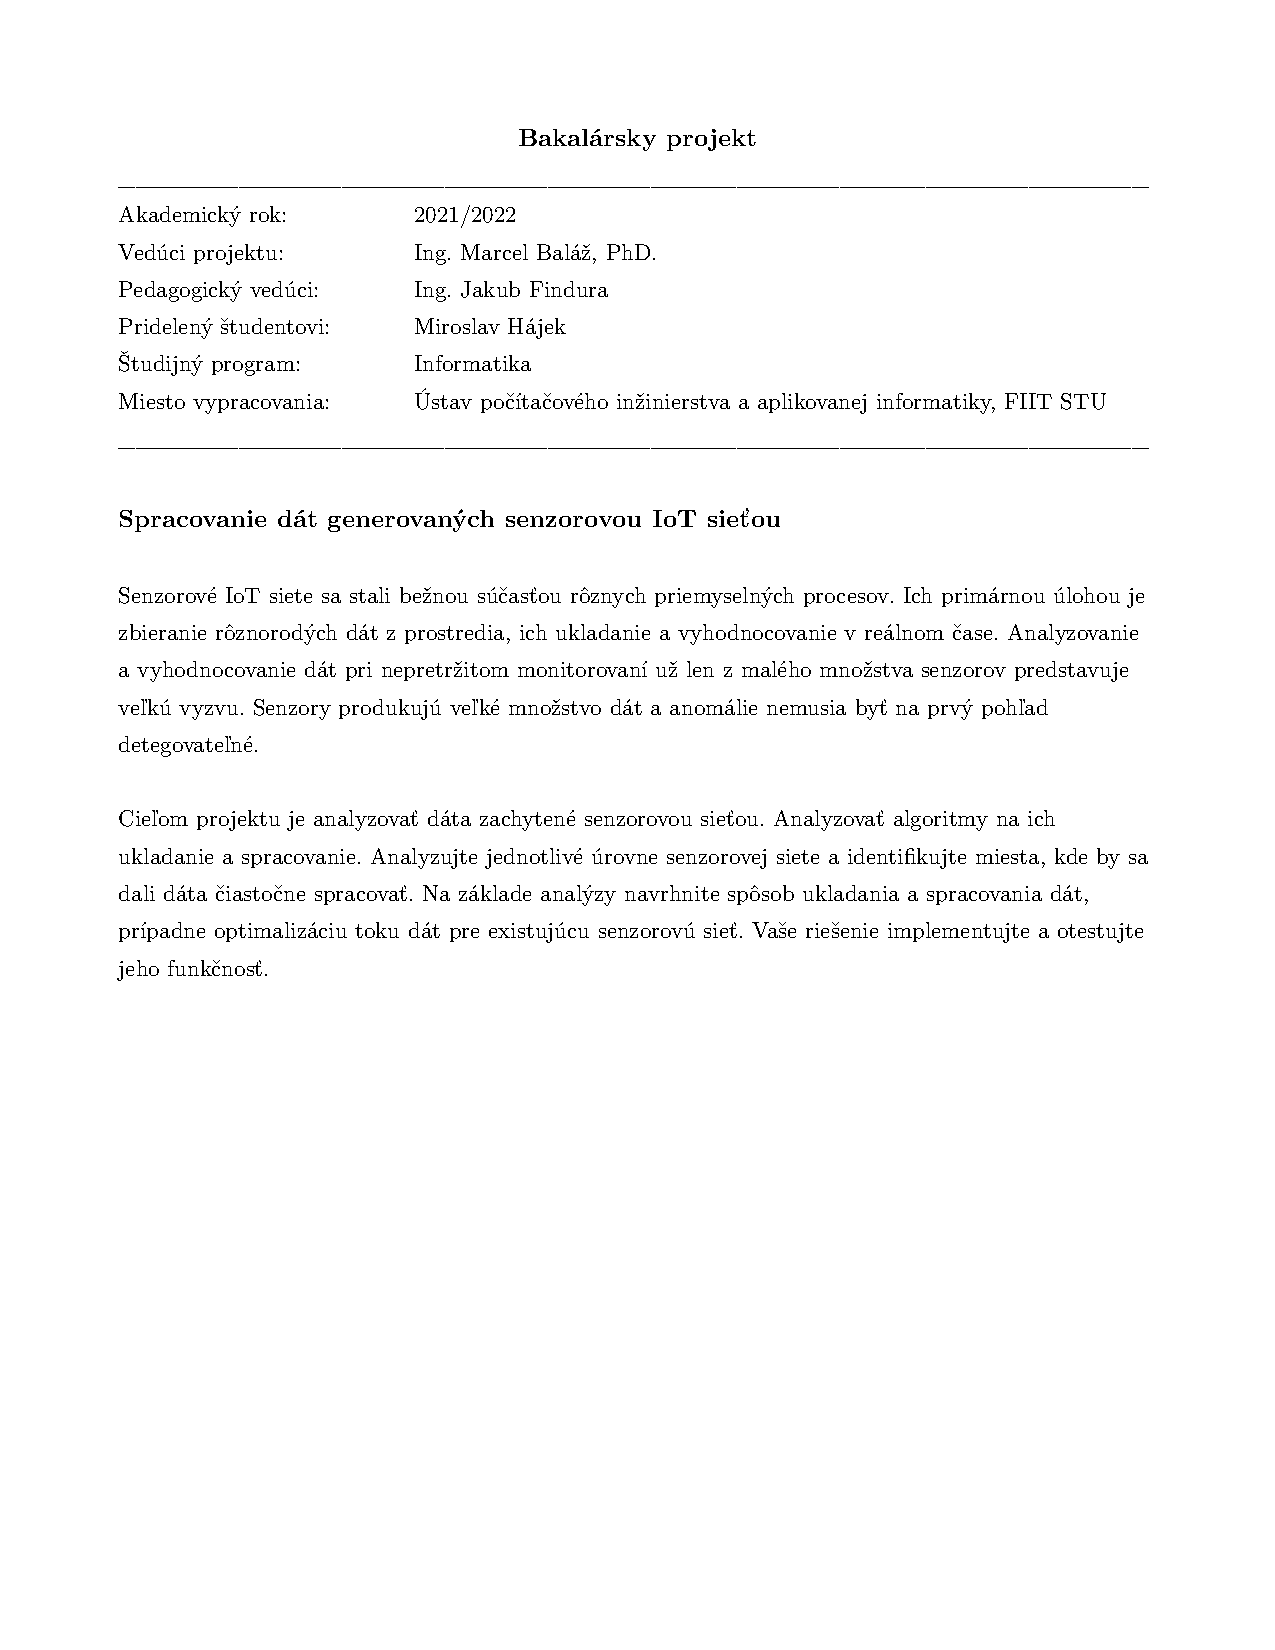
\includepdf[pages=1]{zadanie}
\emptypage

 % Čestné prehlásenie
\thispagestyle{empty}
\vspace*{\fill}
\section*{Čestné prehlásenie}
Čestne vyhlasujem, že som túto prácu vypracoval samostatne, na základe konzultácií
a s použitím uvedenej literatúry.

\vspace{3\medskipamount}\noindent
\SignPlace \SignDate \hspace*{\fill} \signaturespace{5cm}{\Author} 

\emptypage
% Poďakovanie
\thispagestyle{empty}
\vspace*{\fill}
\section*{Poďakovanie}
Chcel by som sa poďakovať vedúcemu práce Ing.~Marcelovi Balážovi,~PhD. za ústretovosť, mnohé cenné pripomienky a podnety k vylepšeniam, usmernenia pri vytýčení zamerania a povzbudenie ku tvorivému preskúmaniu problematiky. 

Za poskytnutie  senzorovej jednotky a za postrehy ku formálnej stránke vďačím Ing.~Lukášovi Doubravskému. 

Tiež ďakujem svojmu kolegovi Ing.~Michalovi Juranyimu, ktorý ma za roky spolupráce mnohému priučil o vývoji softvéru.
Veľmi si cením morálnu podporu popri štúdiu od rodičov a od najbližšieho okruhu spolužiakov -- kamarátov.
\vspace{3cm}
\emptypage
%Anotácia
\thispagestyle{empty}
\section*{Anotácia}
\University \\
\uppercase{\Faculty}
\vspace{-8pt}
{\setlength{\mathindent}{0cm}
\begin{align*}
&\text{Študijný program:} && \text{\StudyProgramme} \\
&\text{Autor:} && \text{\Author} \\
&\text{\Thesis:} && \text{\Title} \\
&\text{Vedúci bakalárskej projektu:} && \text{\Supervisor} \\
&\text{Pedagogický vedúci:} && \text{\PedagogicalSupervisor} \\
&\text{\Date}
\end{align*}}
Stručná charakteristika zadania bakalárskeho projektu ale predovšetkým výsledkov bakalárskeho projektu v slovenskom a anglickom jazyku každá v rozsahu max. 1 strany A4 (hlavička + cca 150-200 slov).
\emptypage

%Anotácia EN
\thispagestyle{empty}
\section*{Annotation}
\UniversityEN \\
\uppercase{\FacultyEN}
\vspace{-8pt}
{\setlength{\mathindent}{0cm}
\begin{align*}
&\text{Degree course:} && \text{\StudyProgrammeEN} \\
&\text{Author:} && \text{\Author} \\
&\text{\ThesisEN:} && \text{\TitleEN} \\
&\text{Supervisor:} && \text{\SupervisorEN} \\
&\text{Departmental advisor:} && \text{\PedagogicalSupervisorEN} \\
&\text{\DateEN}
\end{align*}}
Annotation text in English, 150-200 words.
\emptypage 


% Obsah
\renewcommand{\contentsname}{Obsah}
\pagestyle{empty}
\tableofcontents{}
\listoffigures
\listofmyequations
%\listofalgorithms
{\let\clearpage\relax \printnomenclature}
\emptypage


\pagestyle{fancy}
% Kapitoly
\pagenumbering{arabic}

\chapter{Úvod}
Inteligentné senzorové systémy zariadení internetu vecí zaznamenávajú obrovskú kvantitu údajov z prostredia, kde
pôsobia. Prúdy vzoriek meraných veličín majú samy osebe nízku informačnú hodnotu. Zbytočne zaťažujú
prenosové pásmo komunikačných kanálov a kapacitu úložísk. Monitorovanie širokého rozsahu kladie požiadavky
na nízke výrobné náklady senzorových jednotiek a dlhodobú výdrž pri napájaní z batérií za minimálnej údržby.
Existuje preto potreba získané dáta spracovať do istej miery už v blízkosti ich zdroja, aby došlo k efektívnemu
využitiu dostupných prostriedkov.

Význam a dôležitosť sledovania vibrácií spočíva v ich výskyte u každého mechanického zariadenia pohybom jednotlivých súčiastok
a trením v ložiskách. Ich nadmerná prítomnosť býva spôsobená opotrebením dielov stroja alebo dôsledkom technických defektov.
Ďalšou oblasťou hojnej prítomnosti vibrácií je preprava osôb a tovaru. Tam sú zapríčinené nerovnosťami povrchu vozovky
alebo koľaje v bode styku s kolesami, či aparátom ovplyvňujúcim pohyb vozidla. Menovite ich vyvoláva točivý moment
spaľovacieho alebo elektrického motora a činnosť brzdového systému.

Detekciou nežiaducich vibrácií v preprave sa dokáže zabezpečiť bezpečnosť pasažierov včasnou výmenou súčiastky,
ktorá by ovplyvnila prevádzkyschopnosť v kritických momentoch. Ich odhalením predchádzame nenávratnému poškodeniu krehkých materiálov,
znehodnoteniu reaktívnych substancií, či ich aktivácii v prípade výbušnín a pyrotechniky. Vibrácie sú súčasťou
nebezpečných prírodných úkazov a správna identifikácia má za následok varovania na evakuáciu obyvateľstva
v oblasti postihnutej zemetrasením, či erupciou sopky, vedúcimi k ohrozenia zdravia osôb a poškodenia majetku.

Vibračný signál je merateľný v digitálnej podobe snímačom pohybového zrýchlenia mikromechanickej konštrukcie, o čom
pojednávame v kapitole \ref{chapter:analysis}. Na postupnosť pozorovaní sa nazerá ako vlnový priebeh,
ktorý sa sprehľadňuje agregačnými, korelačnými a testovacími štatistikami na odhalenie náhlych zmien.
Významne úrovne sa odlišujú od nevýznamných algoritmami na detekciu špičiek. Metódami transformácie do frekvenčnej oblasti
sa objavujú periodicky prítomné zložky. Modely spracovania majú byť nasadené do adekvátnej vrstvy senzorovej siete.
V kapitole \ref{chapter:design} popíšeme hardvér, pre ktorý navrhneme firmvér uskutočňujúci sústavu
krokov na extrakciu udalostí z vektora zrýchlenia a predstavíme dátové sady na validáciu funkčnosti.
Ďalej v kapitole \ref{chapter:implementation} je prezentovaná implementácia najdôležitejších štruktúr a komponentov. Nakoniec
riešenie overíme v kapitole \ref{chapter:verification} a dosiahnuté výsledky okomentujeme v kapitole \ref{chapter:evaluation}.




\chapter{Analýza}

\section{Monitorovanie vibrácií a šoku}
Vibrácie sú periodickým kmitaním hmoty okolo rovnovážnej polohy vznikajúce excitáciou látky, ktorej je dodaná potenciálna energia, a zo
zákona zachovania energie je následne premieňaná na kinetickú energiu. V realite dochádza pôsobením trenia k útlmu voľného oscilačného
pohybu s časom  a pohybová energia sa uvoľňuje v podobe tepelnej alebo akustickej emisie do okolitého prostredia. Častejšie ako presné
harmonické kmity sú pozorované náhodné vibrácie, ktorých vývoj nevieme dopredu predvídať. Naproti tomu šok, alebo aj prechodový jav, je
náhle uvoľnenie kinetickej energie krátkeho trvania oproti prirodzenej oscilácii systému.

Význam a dôležitosť sledovania vibrácií spočíva v ich výskyte u každého mechanického zariadenia a je zapríčinená pohybom jednotlivých
súčiastok a trením v ložiskách. Ich nadmerná prítomnosť býva spôsobená opotrebením dielov stroja alebo nevyvážením rotačných častí,
zakliesňovaním ozubených kolies, ako dôsledkoch iných technických defektov. V prevažnej väčšine prípadov ide o nežiaduci jav nakoľko
zakladá zníženiu účinnosti so zvýšením hlučnosti ako vedľajšiemu produktu.

Ďalšou oblasťou hojnej prítomnosti vibrácií je preprava osôb alebo tovaru cestnými a železničnými dopravnými prostriedkami, kde sú
zapríčinené nerovnosťami povrchu vozovky alebo koľaje v bode styku s kolesami vozidla. Na zvýšenie ovládateľnosti vozidla a komfortu
pasažierov sú kabíny odpružené od kolies tlmičmi. Lietadlá sú zasa pod vplyvom trenia vzduchu s trupom a krídlami konštrukcie, ktoré je
ďalej zosilnené vzdušnými prúdmi a turbulenciami.

Druhým významným faktorom podieľajúci sa na tvorbe vibrácii je aparát, ktorý uvádza vozidlo do pohybu alebo zastavuje, čiže hnací
najčastejšie spaľovací, dieselový alebo elektrický motor a brzdový systém. Jedná sa najmä o vplyv pohybu piestov, alebo rotora u
elektrických vozidiel, a prenosu otáčavého pohybu motora cez oje hriadeľa na nápravy. ABS brzdový systém prítomný pri väčšine
automobilov zabraňujú šmyku striedavým zomknutím a uvoľňovaním brzdových kotúčov, čo má tiež vplyv na podmienky počas jazdy.

Detekciou nežiaducich vibrácií v preprave sa dokáže zabezpečiť aj bezpečnosť pasažierov včasnou výmenou súčiastky, ktorá by ovplyvnila
prevádzkyschopnosť v kritických momentoch. Ich eliminácia dokáže predísť nenávratnému poškodeniu krehkých materiálov alebo
znehodnoteniu reaktívnych substancií, či dokonca ich aktivácii v prípade výbušnín a pyrotechniky.

V neposlednom rade sú vibrácie súčasťou potenciálne nebezpečných prírodných úkazov a ich správna identifikácia má za následok varovania
pre preventívnu evakuáciu obyvateľstva v oblasti, ktoré bude zasiahnutá zemetrasením, či erupciou sopky vedúcimi k ohrozenia zdravia
osôb a poškodenia majetku.

\subsection{Meranie fyzikálnej veličiny akcelerácie}
Pohyb mechanického systému vystaveného vonkajším silám sa nazýva odozva, ktorej správanie opisuje zjednodušený model s jedným stupňom
voľnosti (1DOF) kmitajúceho telesa s pružinou a tlmičom \cite{vibrations-shock}.

\begin{figure}[h]
	\centering
	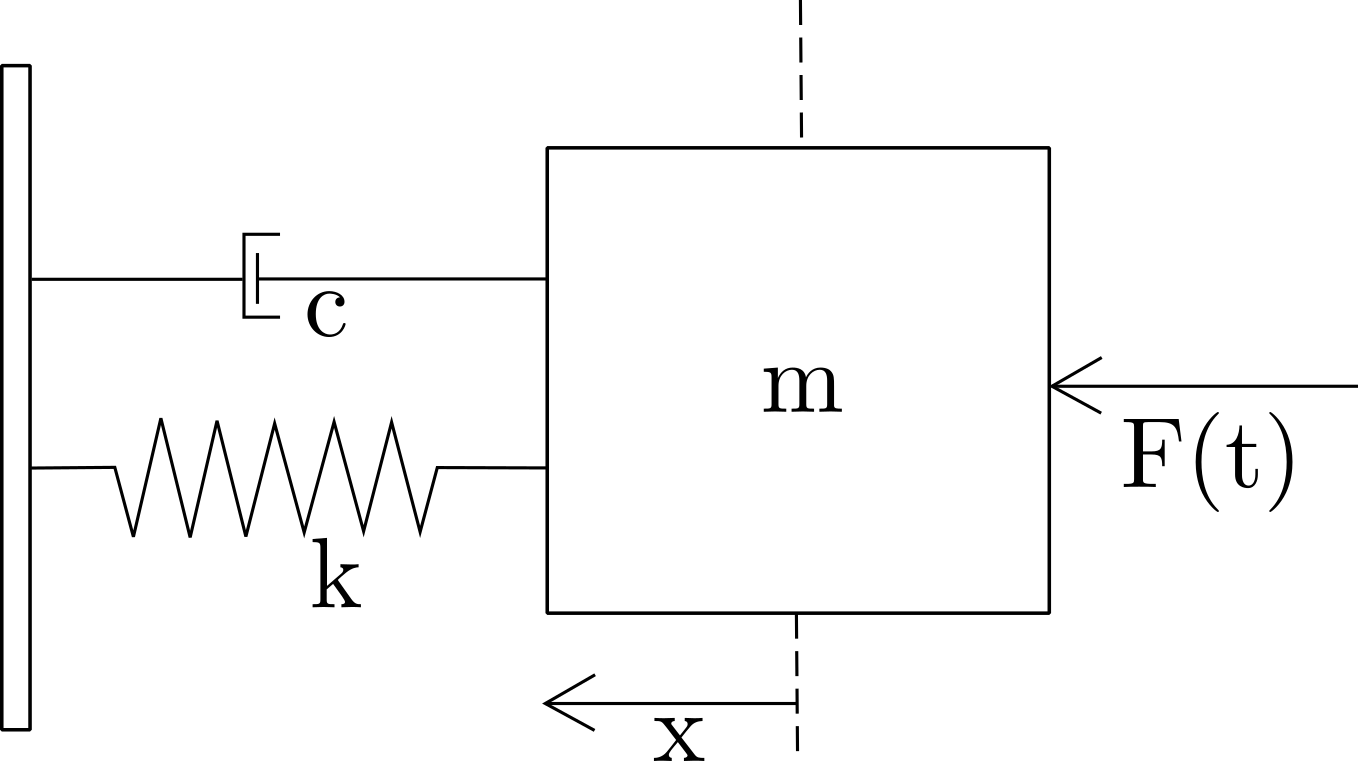
\includegraphics[width=0.7\textwidth]{figures/mass-spring-damper-model.png}
	\caption{Model oscilujúceho systému s pružinou a tlmičom}
\end{figure}

Pri pôsobení vonkajšej sily $F$ na hmotu upevnenú na pružine vznikajú nútené vibrácie, ktoré ju vychyľujú z rovnovážnej polohy.
Uvedená sila je charakterizovaná druhým Newtonovým zákonom v tvare $F = ma$, kde $m$ je hmotnosť telesa a $a$ predstavuje zrýchlenie.
V protismere pôsobí sila vyvolaná pružinou $F_s = -kx$ a tlmiacim členom $F_d = -cv$, kde $k$ je tuhosť pružiny ovplynená jej konštrukciou,
$c$ je tlmiaci koeficient, $x$ je vychýlenie z rovnovážneho stavu, a $v$ rýchlosť vychýlenia.

Fyzickým obmedzením  telesa, ktorým je viazaný na pevnú podložku dochádza pri zanedbaní deformácie k takmer zaručenému návratu do rovnovážnej
polohy a to nám umožňuje merať intenzitu vibrácií cez zrýchlenie ťažidla. Výslednú silu v jednom smere získame sčítaním síl podieľajúcich sa na dynamike telesa.
\myequations{Fyzikálny model oscilujúceho systému s pružinou a tlmičom}
\begin{ceqn}\begin{align}
 	F(t) = ma - cv - kx
\end{align}\end{ceqn}

Pri použití trojosového akcelerometra, kedy sú evidované všetky tri priestorové súradnice časovo-premennej akcelerácie dostávame
nasledujúcu rovnicu vo vektorovom tvare:
\myequations{Newtonov zákon sily}
\begin{ceqn}\begin{align}
   \vec{a}(t) = \frac{\vec{F}(t)}{m}
\end{align}\end{ceqn}

Magnitúda akcelerácie s troma súradnicami je daná $L_2$ normou vektora $\vec{a} = (a_x, a_y, a_z)$:
\myequations{Magnitúda vektora akcelerácie}
\begin{ceqn}\begin{align}
   |a| = \sqrt{a_x^2 + a_y^2 + a_z^2}
\end{align}\end{ceqn}

\subsection{MEMS kapacitný akcelerometer}
Bežné inerciálne senzory na meranie zrýchlenia priamočiareho, ale aj rotačného pohybu (gyroskop), sa vyrábajú technológiou
\emph{MEMS – mikromechanický systém}, kedy je celé zariadenie vrátane všetkých mechanických súčastí umiestnené na kremík procesom
mikrovýroby vo viacerých vrstvách. Sila spôsobujúca zrýchlenie je potom meraná vychýlením vstavanej odpruženej hmoty vzhľadom
na pevné elektródy, ktoré môžu byť usporiadané jednostranne alebo ako diferenčný pár \cite{mdof-mems-accelerometers}.

\begin{figure}[h]
	\centering
	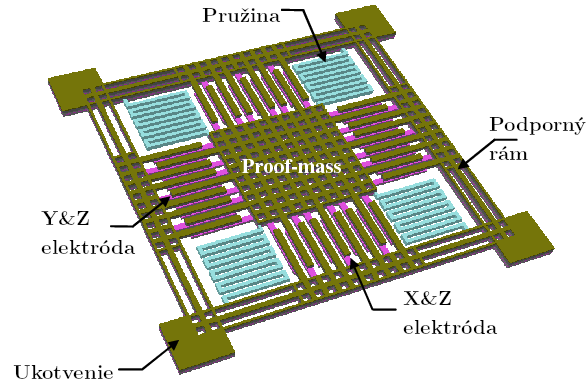
\includegraphics[width=0.8\textwidth]{figures/mems-accelerometer.png}
	\caption{Mikroštruktúra 3DOF MEMS kapacitného akcelerometra \cite{microstructure-mems}}
	\label{fig:mems}
\end{figure}

Pri diferenčnom páre spôsobí pohyb doštičky ťažidla medzi elektródami zmenu kapacít a ich rozdielom je možné zistiť aplikovanú silu a
cez uvedený vzťah zrýchlenie. Na zvýšenie celkovej kapacity sa používa viacero párov elektród zapojených paralelne. Pred prevodom na
číslicový signál musí napäťová úroveň zo senzora prejsť úpravou zahŕňajúcou nábojovocitlivý predzosilňovač, osovú demoduláciu a anti-
aliasingové filtrovanie.

Viacosové akcelerometre vyžadujú viaceré opísané štruktúry orientované kolmo na seba, podľa obr. \ref{fig:mems}, s ohľadom na počet
vyžadovaných stupňov voľnosti, pričom v skutočných senzoroch vždy existuje aspoň minimálna závislosť medzi osami rádovo najviac v
jednotkách percent. Teplota ovplyvňuje citlivosť MEMS akcelerometrov len nepatrne v stotinách percenta na stupeň Celzia.

Akcelerometre sa odlišujú v niekoľkých dôležitých vlastnostiach, ktoré zvyknú byť nastaviteľné vo výrobcom stanovenom rozsahu
prípustných hodnôt s príslušnými toleranciami \cite{accelerometer-mechanics}.

\emph{Citlivosť} stanovuje najmenšiu rozlíšiteľnú zmenu v odčítanom napätí ku zmene externého pohybu respektíve zrýchlenia.
Uvádza sa v jednotkách \emph{mV/g} (milivolt na tiažové zrýchlenie) pri analógovom výstupe, alebo \emph{mg/LSB} (mili-g
na najmenej významový bit). pri senzoroch so vstavaným analógovo-digitálnym prevodníkom. Jednotka \emph{mg/LSB} vyjadruje
o koľko sa zmení zrýchlenie keď zvýšime alebo ponížime binárne číslo na výstupe o jedna. Niekedy sa namiesto
citlivosti uvádza mierka pre presnosť ako prevrátená hodnota citlivosti v \emph{LSB/g}. Tiažové zrýchlenie $g$ sa mierne líši podľa
zemepisnej šírke, ale stanovený prepočet na jednotky SI je $1 g = 9.80665\,m/s^2$
\footnote{\url{https://physics.nist.gov/cgi-bin/cuu/Value?gn|search_for=acceleration}}.

\emph{Dynamický rozsah} sa uvádza v tiažovom  zrýchlení $g$. Hovorí o najmenšej a najväčšej rozlíšiteľnej hodnote zrýchlenia nad
úrovňou ktorej už dochádza k skresleniu signálu orezaním špičiek. S nevyhnutnými drobnými nepresnosťami výroby mikromechaniky je tzv.
\emph{zero-g napätie} popisujúce odchýlku skutočného od ideálneho výstupu, keď na sústavu nepôsobí žiadne zrýchlenie. Za ideálnych
okolností bez pohybu na vodorovnom povrchu namerajú osi $x$ a $y$ zrýchlenie $0g$, zatiaľčo na $z$ pôsobí $1g$. Očakávaním je nulová
hodnota výstupného napätia a tým aj výstupného registra.

\emph{Šírka pásma} senzora v \emph{Hz} predurčuje rozsah frekvencie vibrácií, ktoré je možné zachytiť. Podmienená je zvolenou
početnosťou  čítania akcelerácie za sekundu, čiže vzorkovacou frekvenciou. Stanovuje sa tiež nastaviteľným parameterom \emph{ODR}
(Output Data Rate) - výstupný dátový tok, pričom šírka pásma je spravidla polovicou ODR. Menej uvádzanou vlastnosťou býva
\emph{frekvenčná odozva} senzora, ktorá určuje o koľko sa v rámci tolerancie odlišuje skutočná
citlivosť od referenčnej pre zodpovedajúcu frekvenciu vibrácii.

Na meranie zrýchlenia má nevyhnutný vplyv šum zapríčinený Brownovým  pohybom a nedokonalosťou skutočných materiálov v štruktúre
akcelerometra. Intenzita šumu rastie inverznou odmocninou so šírkou pásma, čiže s častejším meraním získavame menšiu presnosť. Pri
dostatočnom odstupe signálu od šumu, $SNR = P_{signal} / P_{šum}$, umožňuje hardvér akcelerometra vzorkovať amplitúdy až nad stanovený
prah generovaním prerušenia, čím sa dokáže efektívne zbaviť nevýznamných fluktuácií.

\subsection{Analógovo-digitálny prevodník}
Spojitá napäťová úroveň transformuje analógovo-digitálny (A/D) prevodník pre spracovanie digitálnym systémom do množiny diskrétnych
hodnôt. Vstupný signál najprv prechádza fázou vzorkovania, kedy sa vzorky zaznamenávajú v pravidelných intervaloch. Počet vzoriek
odčítaných za sekundu je vyjadrený vzorkovacou frekvenciou $f_s$ v $Hz$. Časový rozdiel medzi vzorkami, nazývaný perióda vzorkovania,
je prevrátenou hodnotou vzorkovacej frekvencie $T_s = \frac{1}{f_s}$. Pre presnú rekonštrukciu pásmovo obmedzeného signálu v hraniciach
$[-f_{max}; f_{max}]$ je nevyhnuté podľa \emph{Nyquist-Shannonovej vety} o vzorkovaní, aby vzorkovacia frekvencia bola najmenej
dvojnásobkom maximálnej frekvencie snímaného signálu.
\myequations{Nyquist-Shannonova veta o vzorkovaní}
\begin{ceqn}\begin{align}
   f_s \geq 2 \cdot f_{max}
\end{align}\end{ceqn}

V procese kvantovania je každej vzorke je následnepriradená diskrétna hodnota s konečným počtom $n$ bitov, ktorá je najbližšia
možná ku skutočnej hladine analógového vstupu. Dochádza pritom k istému zaokrúhľovaniu z dôvodu nepresnosti vyjadrenia spojitej
domény amplitúd diskrétnym číslom. Tento jav označujeme ako kvantizačný šum, ktorý je najviac polovicou z maximálnej rozlíšiteľnej
zmeny signálu a trpia nim všetky existujúce A/D prevodníky.

\begin{figure}[h]
	\centering
	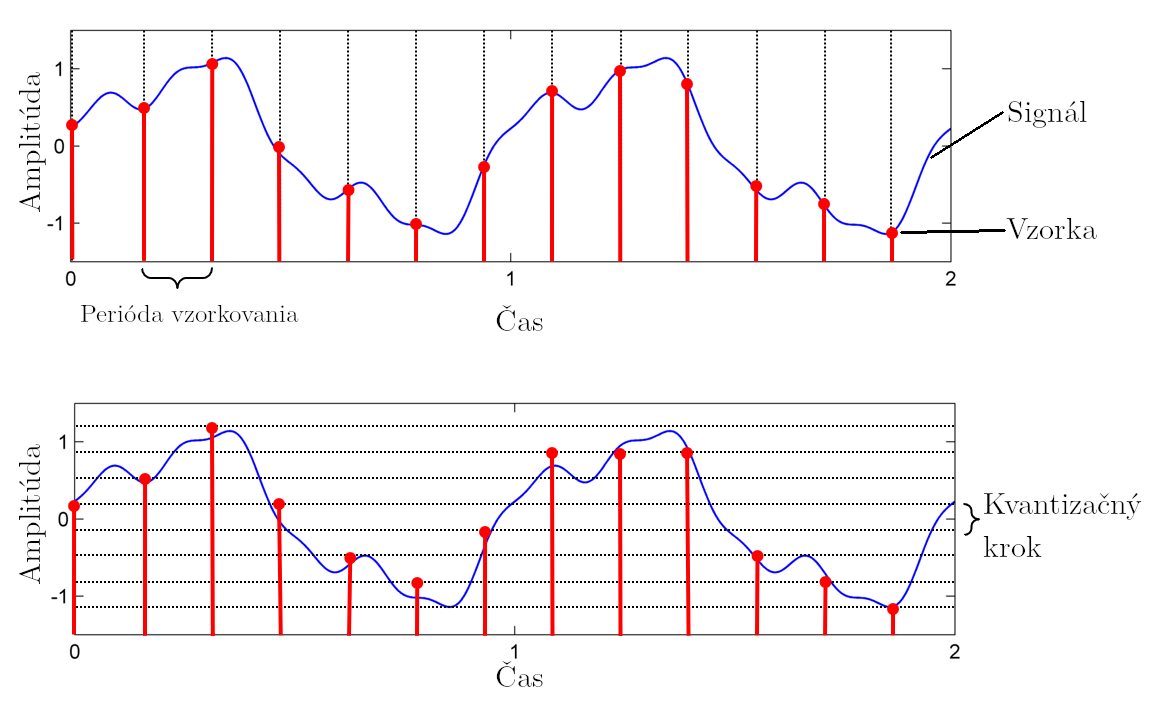
\includegraphics[width=0.8\textwidth]{figures/analog-to-digital-conversion.png}
	\caption{Digitalizácia signálu v analógovo-digitálnom prevodníku \cite{music-processing}}
\end{figure}

Prevodníky integrované priamo s inerciálnymi jednotkami sa vyhotovujú v rozlíšeniach 12, 16 alebo 20 bitov. Umožňujú tak pripojiť
akcelerometer rovno na sérové zbernice \emph{SPI} alebo \emph{I2C}. Všeobecne platí, že pri $n$ bitoch je k dispozícii $2^n$ rozličných
čísel. Kódovaním v dvojkovom doplnku pre zachytenie záporných hodnôt sa uvažuje s intervalom $[-2^\frac{n}{2}; 2^\frac{n}{2} - 1]$.

Číslicová hodnota v dvojkovom doplnku získanú konverziou $\hat{x}$ je prepočítaná na
štandardné fyzikálne jednotky pre zrýchlenie, $a$ v $m/s^2$). $R$ prestavuje nastavený dynamický rozsah v jednotkách $g$ a $n$
je počet bitov A/D prevodníka.
\myequations{Konverzia merania na akceleráciu podľa rozlíšenia A/D prevodníka}
\begin{ceqn}\begin{align}
   a = \hat{x} \cdot ((R \cdot g) / 2^{n / 2})
\end{align}\end{ceqn}

Na základe už zmieneného ohľadom vlastností MEMS akcelerometrov, presnejší prevod dosiahneme zužitkovaním deklarovanej citlivosti
senzora pri danom dynamickom rozsahu $S_R$ udávaného v $mg/LSB$.
\myequations{Prevod A/D prevodníkom u akcelerometra s rozsahom v $mg/LSB$}
\begin{ceqn}\begin{align}
   a = \hat{x} \cdot (S_R \cdot g) / 1000
\end{align}\end{ceqn}

\subsection{Vlastnosti bežných akcelerometrov}
Na ilustráciu uvádzame parametre zvolených najrozšírenejších typov akcelerometrov. Akcelerometer LSM9DS1 \cite{lsm9ds1} umožňuje cez
zbernicu SPI alebo I2C zvoliť zo štyroch dynamických rozsahov, pričom každé rozpätie sa vyznačuje svojou citlivosťou. Zvolením menšieho
dynamického rozsahu zvýšime citlivosť. LSM9DS1 funguje pri rozsahoch $\pm2$g, $\pm4$g a $\pm8$g a $\pm16$g, postupne s citlivosťami
$0.061$ mg/LSB, $0.122$ mg/LSB, $0.244$ mg/LSB, $0.732$ mg/LSB. Výstupný dátový tok (ODR) je možné nastaviť na $10$Hz, $50$Hz,
$119$Hz, $238$Hz, $476$Hz a najvyššie na $952$ Hz. Navzorkované hodnoty sú ukladané do 16-bitového výstupného registra v
dvojkovom doplnku.

Nízkoenergetický 3DOF MEMS akcelerometer ADXL362 \cite{adxl362} so spotrebou $2\,\mu A$ pri $100$Hz disponuje
rozsahmi $\pm2$g, $\pm4$g a $\pm8$g s citlivosťami $1$, $2$ a $4$ mg/LSB. Dostupné vzorkovacie frekvencie 12-bitového A/D prevodníka sú
$12.5 - 400$Hz v 8 krokoch vždy po násobkoch predošlého kroku. Pre rýchlejšie čítanie pri nižšom rozlíšení dokáže senzor zakódovať dáta
do 8-bitového registra.

Vyrábajú sa tiež akcelerometre s väčšími dynamickými rozsahmi a nízkym šumom, ide napríklad o ADXL356 a ADXL357 \cite{adxl357} so
škálami $\pm 10$g, $\pm 20$g a $\pm 40$g s citlivosťou $0,019$ mg/LSB po $0,078$ mg/LSB a rozlíšením A/D prevodníka 20 bitov pri
ODR $4 - 4000$Hz. ADXL357 ponúka priamo analógové výstupy s citlivosťou $20 - 80$ mV/g pri napájaní $3.3$ V.

\subsection{Odvodzovanie rýchlosti a dráhy zo zrýchlenia}
Meranie akcelerácie umožňuje zároveň nepriamo získať ďalšie údaje o pohybe celkovom v priestore ako aj spôsobenom vibráciami.
Zrýchlenie $\vec{a}$ je definované ako časová zmena rýchlosti $\vec{v}$, zatiaľčo rýchlosť je časovou zmenou polohy $\vec{r}$. Na
pozorovanie prechodových javov alebo na vyjadrenie miery plynulosti pohybu slúži ryv $\vec{j}$, ktorý je časovou zmenou akcelerácie.
Pokiaľ nie sú známe počiatočné podmienky v okamihu začiatku snímania akcelerácie, budú hodnoty veličín relatívne vzhľadom na
štart záznamu. Kinematika v diskrétnom čase je potom opísaná nasledujúci rovnicami, kde $\Delta$ je operátor diferencie
$\Delta t = t(i) - t(i-1)$:
\myequations{Kinematické rovnice pre polohu, rýchlosť, zrýchlenie a ryv}
\begin{ceqn}\begin{align}
   \vec{v} = \frac{\Delta \vec{r}}{\Delta t}; \;\;
   \vec{a} = \frac{\Delta \vec{v}}{\Delta t}; \;\;
   \vec{j} = \frac{\Delta \vec{a}}{\Delta t}
\end{align}\end{ceqn}

Vyjadrenie neznámych premenných vzhľadom na akceleráciu spočíva v prenásobení rovníc členom $\Delta t$, čím sa získajú
vzťahy pre okamžitú dráhu a okamžitú rýchlosť. Spočítaním čiastkových okamžitých rýchlostí na intervale dostaneme celkovú rýchlosť a
rovnaký úsudok platí pre polohu. V spojitom čase, keď by vzorkovacia perióda bola nekonečne krátka, dochádza naproti tomu k
integrovaniu funkcie akcelerácie. Dostávame, že rýchlosť je integrálom zrýchlenia a poloha je dvojným integrálom zrýchlenia:
\myequations{Rýchlosť a poloha cez integrál akcelerácie}
\begin{ceqn}\begin{align}
   \vec{v}(t) = \vec{a_0} + \int{\vec{a}(t)\,\mathrm{dt}} \\
   \vec{r}(t) = \vec{r_0} + \vec{v_0}t + \iint{\vec{a}(t)\,\mathrm{dt}}
\end{align}\end{ceqn}


\subsection{Numerická kvadratúra}
Približný výpočet určitého integrálu funkcie akcelerácie je založený na geometrickej interpretácii integrálu ako plochy pod krivkou.
Hovoríme vtedy o probléme numerickej kvadratúry, ktorý navrhuje nahradiť pôvodný integrand interpolačným polynómom
\cite{numerical-mathematics}. Rád polynómu $n$ implicitne stanoví priebeh funkcie medzi ekvidištantnými vzorkami a
má dopad na presnosť aproximácie. Najčastejšie sa používajú konštantný ($n = 0$), lineárny ($n = 1$) alebo kvadratický ($n = 2$)
polynóm, podľa toho rozlišujeme obdĺžnikové pravidlo (vzorec \ref{eq:midpoint-rule}),
lichobežníkové pravidlo (vzorec \ref{eq:trapezodial-rule}) a Simpsonovo pravidlo (vzorec \ref{eq:simpson-rule}).
\myequations{Pravidlá numerickej kvadratúry: obdĺžníkové, lichobežníkové, Simpsonovo}
\begin{ceqn}
\begin{align}
   v(t_i) &= T_s \cdot a\left(\frac{t_i + t_{i-1}}{2}\right)  \label{eq:midpoint-rule} \\
   v(t_i) &= \frac{T_s}{2} \cdot [a(t_i) + a(t_{i-1})]		\label{eq:trapezodial-rule} \\
   v(t_i) &= \frac{T_s}{3} \cdot [a(t_{2i}) + 4a(t_{2i - 1}) + a(t_{2i - 2})] \label{eq:simpson-rule}
\end{align}
\end{ceqn}

Pri \emph{obdĺžníkovom pravidle} (obr. \ref{fig:midpoint-rule}) nepripúšťame zmenu hodnoty zrýchlenia medzi vzorkami a okamžitú
rýchlosť, čiže plochu, odhadneme ako dĺžku intervalu vzorkovania vynásobenú priemerom výšok dvoch následných pozorovaní. Interpolačný
polynóm je konštantná funkcia. \emph{Lichobežníkové pravidlo} (obr. \ref{fig:trapezodial-rule}) uvažuje s lineárnou zmenou veličiny
medzi meraniami, preto interpoluje priamkou.\emph{Simpsonovo pravidlo} (obr. \ref{fig:simpson-rule}) sa snaží o ešte tesnejší odhad s
využitím kvadratickej funkcie. Každé kvadratúrne pravidlo sa síce vyznačuje presne vyčísliteľnou chybovosťou, ale k tomu je nevyhnutné
poznať analytické vyjadrenie vibrácií, čo dáva realistický odhad len pri čisto periodických kmitoch.

\begin{figure}[h]
\centering
\begin{subfigure}[b]{0.32\textwidth}
    \centering
    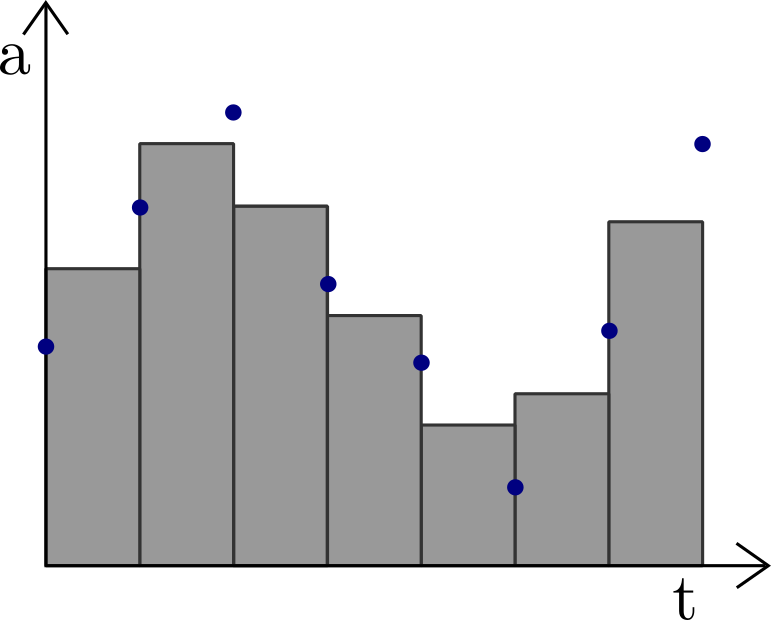
\includegraphics[width=\textwidth]{figures/rectangular-rule.png}
    \caption{Obdĺžníkové}
    \label{fig:midpoint-rule}
\end{subfigure}
\hfill
\begin{subfigure}[b]{0.32\textwidth}
    \centering
    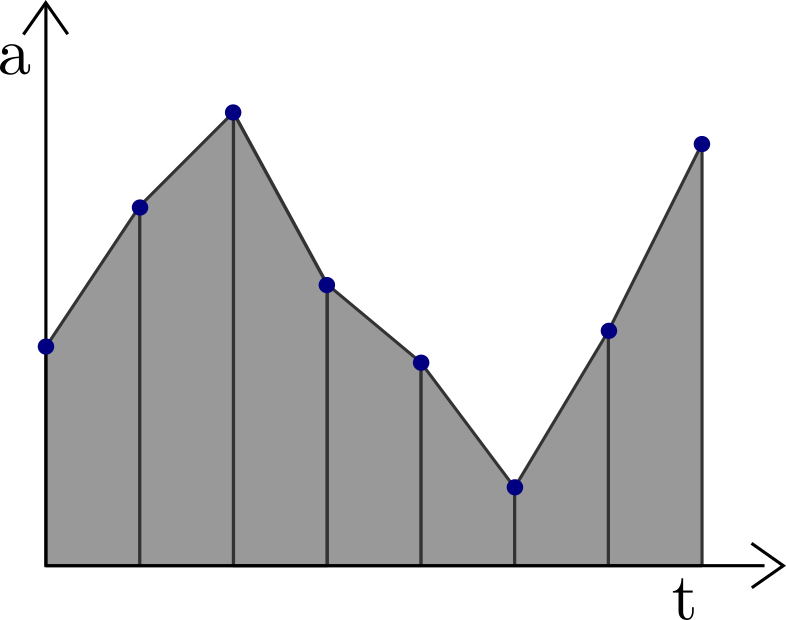
\includegraphics[width=\textwidth]{figures/trapezoidal-rule.png}
    \caption{Lichobežníkové}
    \label{fig:trapezodial-rule}
\end{subfigure}
\hfill
\begin{subfigure}[b]{0.32\textwidth}
    \centering
    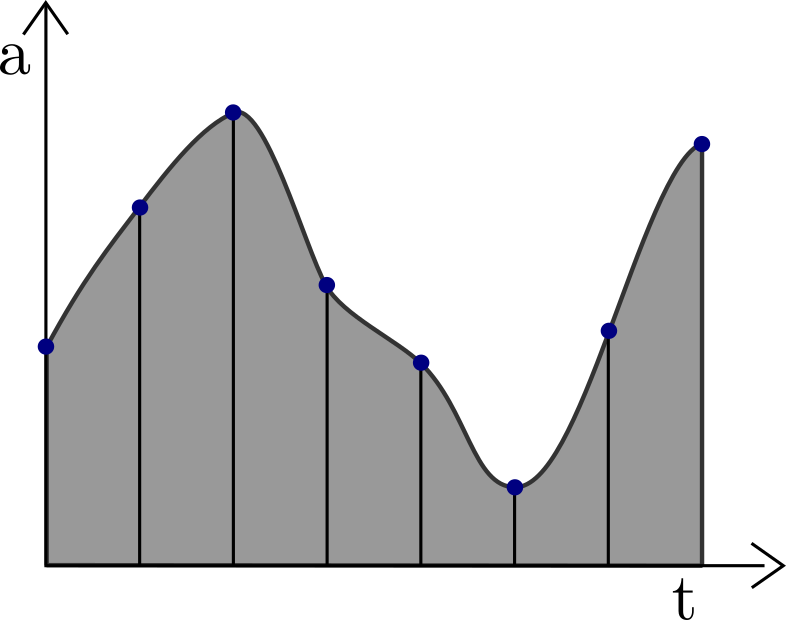
\includegraphics[width=\textwidth]{figures/simpson-rule.png}
    \caption{Simpsonovo}
    \label{fig:simpson-rule}
\end{subfigure}
\caption{Porovnanie pravidiel numerickej integrácie}
\end{figure}

Priama integrácia zašumeného signálu zrýchlenia vedie k neskutočnému driftu, ktorý je ešte zvýraznený dvojitou integráciou pri
odvodzovaní relatívneho posunutia. Dochádza k zosilneniu nízkych a potlačeniu vyšších frekvencií, čím sa začne dominovať neexistujúci
trend vo výstupných dátach. Očakávané oscilujúce správanie vychýlenia u vibrácií so zväčšujúcim sa počtom sčítancov pri rekurentnom
výpočte zaniká. Na zlepšenie stability integrátora sa uplatňuje korekcia cez obálky \cite{integration-acceleration-envelopes}.

Najprv je na vstupnom signále vykonaná zvoleným pravidlom numerická kvadratúra, ktorá môže byť realizovaná na krátkych
úsekoch funkcie, aby sa predišlo pretečeniu pri výraznej akumulácií odklonu. Prichádza k identifikácií lokálnych extrémov a ich interpoláciou s kubickou B-spline sa sformuje horná $e_u(t)$, respektíve dolná
obálka signálu $e_d(t)$. Obálky sú spriemerované $\bar{e}(t)$ za vzniku odhadu trendovej krivky, ktorá je od už integrovaného
signálu odčítaná $g(t) = f(t) - \bar{e}(t)$. V prípade výpočtu polohy je možné aplikovať uvedený postup kaskádovito, čiže rovnako
ako akcelerácia je aj signál rýchlosti opäť integrovaný a korigovaný obálkami.

\section{Metódy analýzy signálu v časovej doméne}
Pozorovania veličiny predstavujú udalosti merané sekvenčne v čase, kde je s každou obdržanou hodnotou $x_i$ viazaná unikátna
časová značka $t_i$. Postupnosť jednotlivých čítaní je jednorozmerný časový rad znázoriteľný ako usporiadaná množina dvojíc pečiatky
rastúcej v čase a nasnímanej úrovne: $T = \{(t_1, x_1),(t_2, x_2), …, (t_n, x_n)\}$. Vzorkovaním v pravidelných intervaloch stačí
uvažovať namiesto časových značiek o celočíselných indexoch, ktoré určujú pozíciu prvkov vo vektore pozorovaní:
$\mathbf{x} = (x_1, x_2, …, x_n)^T$.

\subsection{Prúdové algoritmy}
Pri veľkom objeme prichádzajúcich vzoriek produkované senzormi, nie je uskutočniteľné ich úplné uchovanie ani spracovanie celkého
dátového toku naraz. Častokrát by stratégia neuváženého odkladania viedla k plýtvaniu zdrojov a zbytočnému archivovaniu údajov s nízkou
informačnou hodnotou. Vhodnejšie je agregovanie toku údajov podľa preddefinovaného zmysluplného kritéria, ktoré zachytáva
významné rysy a prompte zodpovedať na vyžadované dopyty.

Priamočiarou realizáciou agregácie je nahliadať na prvky časového radu postupne ako prichádzajú.
Prúdové algoritmy pôsobiace v reálnom čase, a teda neschopné vidieť finálny vektor vzoriek vstupu sa vyznačujú vlastnosťou, že
vyprodukujú len na základe takého čiastkového vstupu parciálny výsledok platný pre dosiaľ sa vyskytnutú podmnožinu.

Za ideálnych okolností by sa mal online algoritmus učiť kontinuálne bez ukladania predošlých bodov a detekcií.
V rozhodnutiach algoritmu sú zahrnuté informácie o všetkých predošlých bodoch do terajšieho rozhodnutia.
Mal by mať schopnosť sa adaptovať dynamickému prostrediu, v ktorom pôsobí, bez nutnosti manuálnych úprav parametrov modelu.
Zároveň je žiaduce minimalizovať falošné pozitíva a negatíva pri detekcii udalostí. \cite{data-streams}.

\subsection{Posuvné a rozširujúce sa okná}
Časový rad $\left(x_i\right)_{i = 0}^{n}$ s dĺžkou $n$ môže byť pre účely výpočtu sumárnych štatistík rozdelený oknovou funkciou
$\mathcal{W}_{l, d}$ na podpostupnosti nazývané okná.

\emph{Posuvné okná} (,,rolling window'') majú spravidla konštatnú dĺžku $l$
menšiu ako celkovú veľkosť radu a sú aplikované s krokom odstupu $d$ pozorovaní. Rad pozorovaní pozostáva z $ (n - (l  - 1)) / d$
okien \cite{online-anomaly-detection}. Prirodzene sa posuvné okná objavujú pri manipulácii s vyrovnávacou pamäťou, ktoré sa využívajú
pri blokovom prenose z adaptéra senzora do hlavnej pamäte. Vtedy sa veľkosť bloku sa rovná posunu $l = d$.

\emph{Rozširujúce sa okná} (,,expanding window'') nachádzajú uplatnenie v menej prípadoch, spravidla sa jedná o inkrementálny
odhad globálnej štatistiky, ktorá má zmysel prevažne pri sledovaní stabilného javu. \cite{practical-time-series}. Okno začína na
stanovenej minimálnej veľkosti a s pribúdajúcim počtom bodov ich zahŕňa, čím sa zväčšuje.

\subsection{Číselné charakteristiky štatistického rozdelenia}
Náhodné vibrácie vyskytujúce sa pri skutočných materiáloch sú stochastický proces, ktorý tvorí sekvencia časovo indexovaných
náhodných premenných. Časový rad predstavuje realizáciu tohto stochastického procesu $\mathbf{Y} = (X_1, X_2, ..., X_n)^T$, kde $X_t$
je náhodná premenná so svojím rozdelením pravdepodobnosti. Všeobecne sa pri ideálnych stacionárnych otrasoch predpokladá, že premenné
pochádzajú z unimodálnej Gaussovej distribúcie: $X_t \sim N(\mu, \sigma^2)$ \cite{vibrations-shock}.

Sumárna deskripcia nameraného deja pre extrakciu typických čŕt konkrétnych pozorovaných situácií sa uskutočňuje viacerými štatistikami
$h(X_1, X_2, ..., X_n)$ zostručňujúcimi opis funkcie hustoty rozdelenie. Na rozmiestnenie hodnôt meraní v priebehu časového úseku
sa nazerá z pohľadu polohy, rozptýlenosti a tvaru. Rozsah oboru hodnôt je amplitúda špička-špička (,,peak-to-peak''),
ktorá je rozdielom maximálnej a minimálnej úrovne, údaj známy tiež ako variančné rozpätie \cite{zaklady-statistiky}.
\myequations{Amplitúda špička-špička}
\begin{ceqn}\begin{align}
x_{pp} = \max_{t \in \mathcal{W}}\{x_t\} - \min_{t \in \mathcal{W}}\{x_t\}
\end{align}\end{ceqn}

Priemernú energiu obsiahnutú v signále predstavuje štvorec efektívnej amplitúdy RMS a určí sa ako kvadratický priemer pozorovaní:
\myequations{Efektívna amplitúda RMS}
\begin{ceqn}\begin{align}
x_{rms} = \sqrt{\frac{1}{n}\sum_{t=1}^{n}{x_t^2}}
\end{align}\end{ceqn}

Mierami polohy rozdelenia pozorovaní sú stredná hodnota, informujúca
o centre hodnôt veličiny, a kvantily rozkladajúce usporiadaný vektor pozorovaní na určený počet rovnakých skupín.
Nevychýleným bodovým odhadom strednej hodnoty je \emph{výberový priemer}, ktorý je zároveň amplitúdou jednosmernej zložky signálu:
\myequations{Výberový priemer alebo amplitúda jednosmernej zložky}
\begin{ceqn}\begin{align}
\bar{x} = \frac{1}{n} \sum_{t = 1}^{n}{x_t}
\end{align}\end{ceqn}

Najvýznamnejším kvantilmi sú kvartily $Q_q$ vytvárajúce štyri rovnako veľké časti z pôvodných dát, konkrétne dolný kvartil $Q_1$
oddelí  25\% najmenších údajov, medián $Q_2$ predelí zoradené údaje na polovicu a horný kvartil $Q_3$ zahrnie 75\% nižších hodnôt.
Hľadaný kvartil je $k$-ty najmenší prvok v utriedenom zozname meraní, pričom podľa želaného kvartilu $q$ a počtu pozorovaní je
$k = \lceil n \cdot (1 / q) \rceil$.

Zistenie $k$-teho najmenšieho prvku s časovou zložitosťou $\mathcal{O}(n \log n)$ umožňuje ľubovoľný lepší triediaci algoritmus
napríklad triedenie zlučovaním (merge sort). Algoritmus \emph{Quickselect} dokáže taký prvok objaviť v čase $\mathcal{O}(n)$.
V každom kroku vyberie náhodný deliaci bod (pivot) a preskupí k sebe hodnoty menšie ako pivot naľavo a väčšie ako pivot
napravo. Najmenší prvok následne hľadá v časti, kde zostalo viac ako $k$ prvkov. Pokiaľ došlo k deleniu zoznamu, že pivot
zaujme presne $k$-tu pozíciu prehľadávanie je ukončené a pivot prehlásený za riešenie. Nesprávnym výberom pivota môže
v najhoršom prípade dôjsť až k zložitosti $\mathcal{O}(n^2)$, čomu sa predchádza výberom pivota cez medián mediánov.

Sústreďovanie realizácie veličiny, respektíve jej rozptýlenosť okolo strednej hodnoty vieme opísať viacerými štatistikami
ako sú \emph{výberový rozptyl} (\ref{eq:variance}), ktorej odmocninou dostaneme smerodajnú odchýlku,
\emph{priemerná absolútna odchýlka} (\ref{eq:aad}), \emph{mediánová absolútna odchýlka} (\ref{eq:mad})
a \emph{medzikvartilové rozpätie} (\ref{eq:iqr}) \cite{zaklady-statistiky}. Priemerná absolútna odchýlka je
upraviteľné o mieru centrálnej tendencie, ktorou okrem priemeru môže byť aj medián alebo modus. Vyvarovanie sa
príliš extrémnym a vychýlením hodnotám docielime zapojením práve mediánu do štatistík absolútnej odchýlky, rovnako
tak to dosiahneme medzikvartilovým rozpätím obmedzením sa na 50\% centrálnych dát.
\myequations{Výberové miery rozptýlenosti: rozptyl, smerodajná odchýlka, MAD, IQR}
\begin{ceqn}\begin{align}
	s^2 &= \frac{1}{n - 1} \sum_{t = 1}^{n}{(x_t - \bar{x})^2} \label{eq:variance} \\
	d &= \frac{1}{n} \sum_{t = 1}^{n}(|x_t - \bar{x}|) \label{eq:aad} \\
	\mathrm{MAD} &= med(|x_t - med(\mathbf{x})|) \label{eq:mad} \\
	IQR &= Q_3 - Q_1 \label{eq:iqr}
\end{align}\end{ceqn}

Numericky stabilné bežiace štatistiky priemeru a smerodajnej odchýlky sa udržiavajú cez rekurentné rovnice
\emph{Welfordovho algoritmu} \cite{knuth}. $M_1$ je aktuálna priemerná hodnota údajov v toku a $S_1$ je počítadlo pre
rozptyl, z ktorého je v ktoromkoľvek okamihu získateľná smerodajná odchýlka súboru $\sigma$:
\myequations{Welfordov algoritmus na výpočet výberového rozptylu}
\begin{ceqn}\begin{align}
   M_1 &= x_1;\quad M_k = M_{k-1} + \frac{(x_n - M_{k-1})}{k} \\
   S_1 &= 0; \quad S_k = S_{k-1} + (x_k + M_{k-1})(x_k + M_k)  \\
   \sigma &= \sqrt{S_n / (n - 1)}
\end{align}\end{ceqn}

Tvar distribúcie náhodnej premennej opisujú centrálne momenty šikmosť a špicatosť. Šikmosť $\gamma_1 = \mu^3 / \sigma^3$ udáva skosenie
rozdelenia, pričom platí že záporná šikmosť značí dlhší ľavý chvost a modus funkcie hustoty sa prevažuje napravo. Zatiaľ čo u kladnej
šikmosti je to naopak (obr. \ref{fig:skewness}).

Špicatosť $\gamma_2 = \mu^4 / \sigma^4 - 3$ (obr. \ref{fig:kurtosis}) porovnáva rozdelenie pozorovaní so strmosťou krivky normálneho rozdelenia,
čiže viacej realizácií leží bližšie alebo ďalej od strednej hodnosti. Kladná špicatosť signalizuje strmejšiu
a záporná zasa sploštenejšiu distribúciu. Platí, že $\mu_n $ je priemerom hodnôt $(x_t - \bar{x})^n$.
\begin{figure}[h]
\centering
\begin{subfigure}[b]{0.48\textwidth}
    \centering
    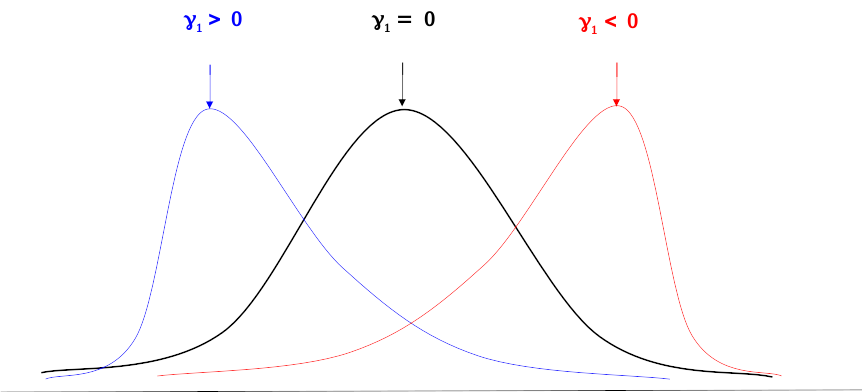
\includegraphics[width=\textwidth]{figures/skewness.png}
    \caption{Šikmosť}
    \label{fig:skewness}
\end{subfigure}
\hfill
\begin{subfigure}[b]{0.48\textwidth}
    \centering
    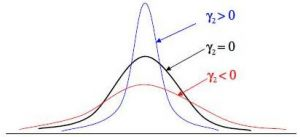
\includegraphics[width=\textwidth]{figures/kurtosis.png}
    \caption{Špicatosť}
    \label{fig:kurtosis}
\end{subfigure}
\caption{Dopad šikmosti a špicatosti na histogram distribúcie}
\end{figure}

Závislosť dvojíc veličín sa vyjadruje \emph{kovariancia} $cov(\mathbf{x}, \mathbf{y})$ a \emph{korelácia}
$\rho(\mathbf{x}, \mathbf{y})$. U vektora akcelerácie nás bude napríklad zaujímať vzájomná korelácia medzi
osami pohybu: $\rho(\vec{x},\vec{y}),\, \rho(\vec{x},\vec{z}),\, \rho(\vec{y},\vec{z})$ upozorňujúca na diagonálny
pohyb alebo podobné budenie v oboch korelovaných smeroch a tým umožňujúce redukciu údajov z dôvodu redundancie.
Kovariancia je daná strednou hodnotou súčinu odchýlky od priemeru zodpovedajúcej premennej (vzťah \ref{eq:covariance}).
Normovaním kovariancie smerodajnými odchýlkami veličín získame \emph{Pearsonov korelačný koeficient}
(vzťah \ref{eq:correlation}), ktorý je z intervalu $[-1; 1]$.  Hodnota koeficientu $-1$ značí nepriamu lineárnu závislosť
a $+1$ priamu závislosť.
\myequations{Závislosť dvoch veličín cez kovarianciu a koreláciu}
\begin{ceqn}\begin{align}
\mathrm{cov}(\mathbf{x}, \mathbf{y}) &= \frac{1}{n} \sum_{t=1}^{n}{(x_t - \bar{x})(y_t - \bar{y})} \label{eq:covariance} \\
\rho(\mathbf{x}, \mathbf{y}) &= \frac{\mathrm{cov}(\mathbf{x}, \mathbf{y})}{\sigma_x \sigma_y} \label{eq:correlation}
\end{align}\end{ceqn}

\subsection{Algoritmy na rozpoznávanie špičiek}
\label{peak-detection}
Detekcia udalostí a významných zmien signálového priebehu sa spolieha na hodnovernú identifikáciu špičiek amplitúdy.
Dôležitými indikátormi pre celkovú charakterizáciu javu slúži potom časová pozícia špičky v rámci prúdu, výška prejavujúca
sa získanou úrovňou, šírka obsahujúca údaj o trvaní, či plocha stvárňujúca energiu.

Ekvivalentne sa špičky z matematického hľadiska stotožňujú s lokálnymi extrémami funkcie, čo sú maximá (vrcholy) a minimá (údolia).
Podľa definície je lokálne maximum $t_0$ bodom, ktorý má vyššiu funkčnú hodnotu ako všetky ostatné body na intervale
$t_0 \in I$ (\ref{equ:local-maxima}), lokálne minimum má na intervale najmenšiu hodnotu (\ref{equ:local-minima})
\cite{survey-peaks-valleys}.
\myequations{Lokálne extrémy funkcie}
\begin{ceqn}\begin{align}
f[t_0] \geq f[t],\, \forall t \in I \label{equ:local-maxima}\\
f[t_0] \leq f[t],\, \forall t \in I \label{equ:local-minima}
\end{align}\end{ceqn}

Kľúčové pre spoľahlivé určenie extrémov je práve interpretácia intervalu $I$ v algoritmoch, ktoré zastupujú rozličné
potreby korektného vyhodnotenia. Jediné minimum a maximum sa dosiahne zvolením celej dĺžky záznamu za interval, čím sa
stratia dočasné disturbancie. Na druhej stane prílišným skrátením intervalu sa skoro všetky vzorky budú javiť ako náhle zmeny.

Skutočné signály sa potýkajú so šumom, ktorý sťažuje odlíšenie pravej tendencie od krátkodobých výkyvov.
Pred samotným procesom hľadania špičiek je preto aplikovaný vyhladzovací filter, v prípade potreby aj opakovane na už
vyhladení signál. Najčastejšie sa jedná o filter
kĺzavého priemeru, Savitzky–Golay alebo Gaussov filter \cite{spectrometry-peak-detection}. Filtrovanie sa realizuje
diskrétnou jednorozmernou konvolúciou vstupného signálu a masky filtra $y[n] = x[n] * w[n]$,
ktorá býva hardvérovo akcelerovaná inštrukciami
,,fused multiply-add''\footnote{\url{https://developer.arm.com/documentation/102198/0200/Convolution}}.

\subsubsection{Detekcia špičiek prahovou úrovňou}
Za predpokladu, že priebeh meranej veličiny sa vyznačuje krátkymi impulzmi s viac-menej pravidelnou amplitúdou
je priamočiarou metódou na odlíšenie špičiek od hladín nízkej aktivity určenie prahu $\theta$, ktorý zaregistruje
všetky väčšie hodnoty. Lokálne extrémy sú potom vzorky signálu spĺňajúce podmienku:
\myequations{Detekcia špičiek prahovou úrovňou}
\begin{ceqn}\begin{align}
|f[t]| \geq \theta
\end{align}\end{ceqn}

Určenie takejto hraničnej hladiny prebieha zväčša empiricky alebo na základe heuristík, ktoré so sebou nesú
domnienku o vlastnostiach priebehu pozorovaní. Uspokojivými odhadom za určitých okolností môžu byť prahy $\theta$:
viac ako priemer s toleranciou, horné $3/4$ celkového nedávneho rozsahu hodnôt, či dokonca viac ako $k$
smerodajných odchýlok. Odlišné nazeranie na prahovú hodnotu spočíva v jej nastavení pre rozpoznanie
vzájomnej korelácie signálu a masky zodpovedajúcej tvaru impulzu. Táto úvaha sa opiera o to, že impulz
musí byť dostatočne pravidelný, aby bol nezameniteľne odlíšiteľný.

\subsubsection{Význačnosť vrchola spomedzi susedov}
Doplnkom ku rozpoznávaniu špičiek podľa absolútnej prahovej úrovne je porovnávanie bodov na
obe strany od preskúmavaného vrchola, čím zistíme relatívnu významnosť extrému pre najbližšie susedstvo.
Aby bola hodnota na danej pozícii $t$ označená za špičku v okolí pozostávajúcom z $k$ priľahlých bodov,
musí byť v porovnaní so všetkými väčšia. Pre okrajové dátové body $f[0]$ a $f[n]$ dochádza k porovnaniu
iba z jednej strany \cite{survey-peaks-valleys}.
\myequations{Význačnosť vrchola spomedzi susedov}
\begin{ceqn}\begin{align}
f[t-i] < f[t] > f[t+i],\quad \forall i \in 1, 2, ..., k
\end{align}\end{ceqn}

Algoritmus č.\ref{algo:neighbours} ,,najvyšší spomedzi susedov''
\footnote{\url{https://terpconnect.umd.edu/~toh/spectrum/PeakFindingandMeasurement.htm}}
prechádza postupne pozorovania veličiny zo zoznamu $y$ a ku kandidátnej špičke na indexe $i$ preveruje najbližších
$k$ hodnôt na obe strany, ak existujú.
\begin{algorithm}[h]
\caption{Najvyšší spomedzi susedov}
\begin{algorithmic}[1]
\Function{Find\_Peaks\_Neighbours}{$y$, $k$, $\varepsilon$, $h_{rel}$, $h$}
	\State $peaks \gets []$ 	\Comment{Zoznam indexov nájdených špičiek v signále $y$}
	\For{$i \gets 0$ \textbf{to} $length(y)$}
		\If {$h \neq null$ \textbf{and} $|y[i]| < h$}  \Comment{Preskoč príliš nízke magnitúdy}
			\State \textbf{continue}
		\EndIf
		\State $possible\_peak \gets true$
		\State $a \gets max(i - k, 0)$
		\State $b \gets min(i + k, length(y))$
		\For{$j \gets a$ \textbf{to} $b$}			\Comment{Porovnaj špičku s bodmi v susedstve}
			\If {$i \neq j$ \textbf{and} $y[j] - y[i] > \epsilon$}
				\State $possible\_peak \gets false$     \Comment{Kopec nie je dostatočne strmý}
			\EndIf
		\EndFor
		\If {$possible\_peak = true$ \textbf{and} $y[i] - \min(y[a], y[b]) > h_{rel}$}
			\State $peaks \gets peaks + [j]$    \Comment{Kandidát je prehlásený za špičku}
		\EndIf
	\EndFor
	\State \Return $peaks$
\EndFunction
\end{algorithmic}
\label{algo:neighbours}
\end{algorithm}
Keď po preskúmaní zostáva $y[i]$ najväčšou hodnotou spomedzi susedov
v rozmedzí $[a; b]$, za tolerancie strmosti stúpania $\varepsilon$ medzi pozorovaniam, a súčasne je relatívna
výška vrcholu väčšia oproti nižšiemu okraju než nastavený parameter $h_{rel}$ potom je kandidátny bod prehlásený
za skutočnú špičku a pridaný do zoznamu $peaks$.

Súčasťou algoritmu je tiež preskočenie hodnôt, ktoré nespĺňajú základný predpoklad pre absolútnu amplitúdu $h$.
Časová zložitosť pre rozhodnutie o jednej špičke je lineárna v závislosti od veľkosti posuvného okna uvažovaného
susedstva $\mathcal{O}(2k)$.

\subsubsection{Algoritmus prechodu nulou do záporu}
Pomyselné vrcholy a údolia v zosnímaných hodnotách sú miestom, kde sa mení smer úrovní amplitúdy zo stúpania na klesanie alebo
z klesania na stúpanie, čím na pomedzí týchto opozitných trendov vzniká stacionárny bod, kde je prvá diferencia nulová:
$\Delta f[i] = 0$. V lokálnom maxime dochádza súčasne k zmene znamienka prvej diferencie z kladného na záporné. Prudkosť
kopca vyplýva z absolútnej hodnoty diferencie.

Viacnásobné vyhladenie signálu predom je nesmierne dôležité,
pretože algoritmus č.\ref{algo:zero-crossing} ,,prechodu nulou do záporu'' (Negative Zero-Crossing) je nesmierne citlivý
na zákmity a nesprávneby ich považoval za špičky. Zvýšenie odolnosti proti takýmto tendenciám sa dosahuje dlhšou sečnicou
spájajúcou bod $i$ s $k$-tou vzorkou vedľa, ktorá sa použije namiesto diferencie s jednotkovým krokom.
\begin{algorithm}[h]
\caption{Prechod prvej derivácie nulou do záporu}
\begin{algorithmic}[1]
\Function{Find\_Peaks\_Zero\_Crossing}{$y$, $k$, $\varepsilon$, $slope$}
	\State $peaks \gets []$
	\For{$i \gets k$ \textbf{to} $length(y) - k$}
		\If {($|y[i+k] - y[i-k]| \leq \epsilon$ \textbf{and}
		     \State \hskip1.5em $(y[i+k] - y[i]) - (y[i] - y[i-k]) < 0$ \textbf{and}
		     \State \hskip1.5em $|(y[i+k] - y[i]) - (y[i] - y[i-k])| > slope$)}
		    \State $peaks \gets peaks + [i]$

		\EndIf
	\EndFor
	\State \Return $peaks$
\EndFunction
\end{algorithmic}
\label{algo:zero-crossing}
\end{algorithm}

Označenie kandidátneho bodu za špičku v zozname hodnôt $y$ stojí na teda troch kritériách. Sklon sečnice sa musí v
rámci tolerancie $\varepsilon$ blížiť nule, rozdiel prvých diferencií $\Delta y[i+k] - \Delta[i]$ musí byť záporný a veľkosť
rozdielu diferencií prekračuje prahovú strmosť kopca $slope$, kde leží uvažovaný vrchol. Časová zložitosť
pre jednu špičku je $\mathcal{O}(1)$.

\subsubsection{Algoritmus horského turistu}
Zanesením do grafu pripomína priebeh funkcie kmitajúceho deja členité pohorie. Na problém rozhodovania sa o tom, či danú lokalitu
považovať za vrchol možno nahliadať z pohľadu chodca cestujúceho po krivke z lineárne interpolovaných vzoriek. V princípe
ide myšlienkou o jednoduchý stavový automat sledujúci aktuálny stav terénu a konajúci rozhodnutia na základe predošlej
skúsenosti v intenciách rozhodovacích pravidiel.

Algoritmus č.\ref{algo:mountain-hiker} horského turistu na začiatku púte z počiatočných bodov zistí, ktorým z dvoch vertikálnych
smerov sa krivka uberá. V prípade, že po druhom kroku dôjde k zmene smeru zapíše sa indikácia možného spádu kopca.
Výchylka môže byť v dôsledku neprekročenia prahových úrovní v horizontálnej ($hole$) a vertikálnej ($tolerance$) osi
ignorovaná, lebo ani na lesnom chodníku sa nepovažuje každá jama alebo vydutie za horu.
\begin{figure}[h]
    \centering
    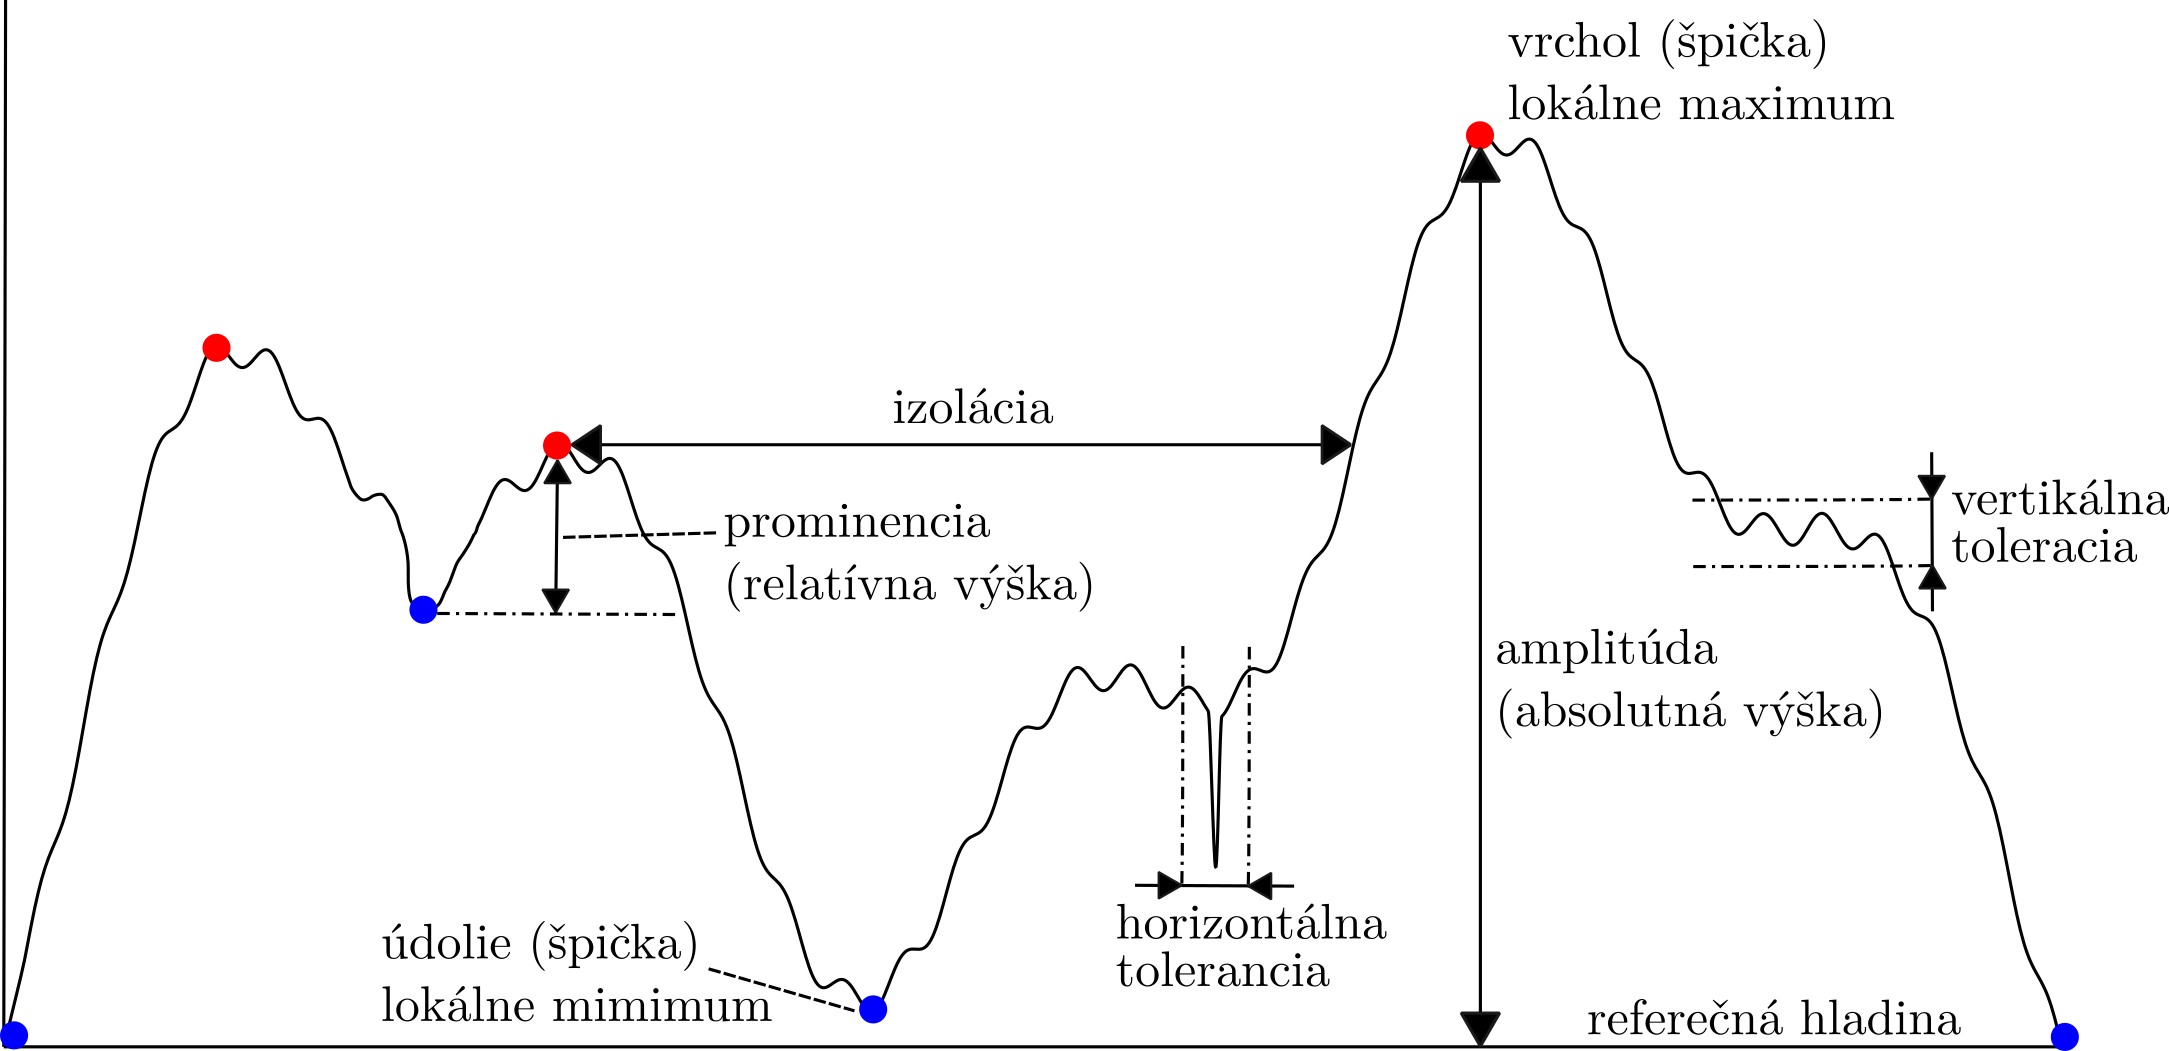
\includegraphics[width=0.9\textwidth]{figures/topography.png}
    \caption{Topografia priebehu signálu}
    \label{fig:topography}
\end{figure}

Domnelý vrchol je označený za lokálne maximum, keď spĺňa parametre pre topografické vlastnosti minimálnej akceptovateľnej
prominencie a izolácie (obr. \ref{fig:topography}. Prominencia znamená relatívnu výšku oproti predošlej navštívenej doline. Izolácia vyčísľuje vzdialenosť k najbližšiemu skoršiemu vrcholu. Podobný algoritmus už existuje v literatúre \cite{peek-mountaineer-method}, avšak nižšie prezentovaný pseudokód je oproti nemu zjednodušený a doplnený o požadované tolerancie.
\begin{algorithm}[h]
\caption{Algoritmus horského turistu}
\begin{algorithmic}[1]
\Function{Find\_Peaks\_Hill\_Walker}{$y$, $tolerance$, $hole$, $prominence$, $isolation$}
	\State $peaks \gets []$
	\State $i\_change \gets 0$
	\State $y\_valley \gets 0$
	\State $possible\_change \gets false$
	\State $uphill \gets (y[1] - y[0]) \geq 0$

	\For{$i \gets 1$ \textbf{to} $length(y)$}
		\State $y\_step \gets y[i] - y[i-1]$
        \State $slope \gets y\_step \geq 0$

        \If {$possible\_change = false$ \textbf{and} $uphill \neq slope$}
        	\State $possible\_change \gets true$   \Comment{Označenie potenciálneho extrému}
        	\State $i\_change \gets i - 1$
        \ElsIf {$possible\_change = true$ \textbf{and} $uphill = slope$}
        	\State $possible\_change \gets false$  \Comment{Potenciálny extrém bol zachvením}
        \EndIf

        \If {($possible\_change = true$
        	\State \hskip1.5em \textbf{and} $uphill \neq slope$
        	\State \hskip1.5em \textbf{and} $|i - i\_change| > hole$
        	\State \hskip1.5em \textbf{and} $|y[i] - y[i\_change]| > tolerance$)}

        	\State $posible\_change \gets False$        \Comment{Významný lokálny extrém potvrdený}
        	\State $prev\_uphill \gets uphill$
        	\State $uphill \gets slope$

        	\If {$prev\_uphill = false$ \textbf{and} $uphill = true$}
				\State $y\_valley \gets y[i\_change]$   \Comment{Nájdené údolie}

            \ElsIf {($prev\_uphill = true$
            		\State \hskip1.5em \textbf{and} $uphill = false$
            		\State \hskip1.5em \textbf{and}  $|y[i - hole] - y\_valley| > prominence$)
            		\State \hskip1.5em \textbf{and}  $|y[i - hole] - y[last(peaks)]| > isolation$)}
				\State $y\_peak \gets y[i\_{change}]$    \Comment{Skutočný vrchol identifikovaný}
				\State $peaks \gets peaks + [i_{change}]$
            \EndIf
        \EndIf
	\EndFor
	\State \Return $peaks$
\EndFunction
\end{algorithmic}
\label{algo:mountain-hiker}
\end{algorithm}
\afterpage{\clearpage}

\subsection{Metriky pre binárny klasifikátor}
Uviedli sme tri rozdielne rovnocenné prístupy odhalenia špičiek. Rozobrali sme algoritmus porovnávajúci susedov na obe strany,
algoritmus využívajúci sklon sečníc vychádzajúc s vlastností prvej derivácie a napokon
stavový automat odvolávajúci sa na sekvenčne preskúmavanú topografiu krivky grafu. Spoločným rysom zmienených techník
je vykonávanie binárne zaradenie pre každú vzorku, či sa sa nachádza alebo nenachádza na aktuálnej pozícii vrchol.

Rozhodnutie môže viesť k správnemu ($P$) alebo nesprávnemu ($N$) riešeniu vzhľadom na objektívnu pravdu
sprostredkovanú anotovanými dátami. Keď sa kategorizácia zhoduje s realitou dostávame skupiny
skutočne pozitívnych $TP$ a skutočne negatívnych $TN$. V prípade, že sa klasifikátor pomýli vyjde buď chyba
prvého rádu $FP$, kedy registrujeme neexistujúcu špičku, alebo chyba druhého rádu $FN$, kedy ju prehliadneme.
Umiestnením počtov charakteru rozhodnutí do tabuľky vzniká matica zámen \cite{binary-classifier}.

Úspešnosť klasifikačných algoritmov pre ich vzájomné porovnanie kvantifikujú viaceré metriky. Na odladenie parametrov
vplývajúcich na náchylnosť preferovať kladné alebo záporné výsledky sa vzťahuje \emph{prevalencia} výskytu očakávaného
javu: $P / (P+N)$ v samotných dátach. Snahou rozhodovania je maximalizovať senzitivitu a špecifickosť výsledkov algoritmu.
\emph{Senzitivita} (\ref{equ:sensitivity}) udáva koľko bodov, ktoré sú prehlásené za špičky naozaj je špičkami.
\emph{Špecifickosť} (\ref{equ:specifity}) sa zameriava na potvrdenie, aké množstvo pozorovaní nepovažovaných za špičky,
nie sú nimi aj skutočne.
\myequations{Metriky klasifikátora: senzitivita a špecifickosť}
\begin{ceqn}\begin{align}
TPR = \frac{TP}{P} = \frac{TP}{TP + FN} \label{equ:sensitivity} \\
TNR = \frac{TN}{N} = \frac{TN}{TN + FP} \label{equ:specifity}
\end{align}\end{ceqn}

Presnosť určenia lokálneho extrému sa skladá z správnosti (\ref{equ:ppv}) a precíznosti (\ref{equ:accuracy}),
ktoré je rovnako žiaduce dosahovať čo najbližšie sto percentám, pri nízkej chybovosti (\ref{equ:error-rate}), čiže
nízkeho počtu falošných poplachov.
\myequations{Metriky klasifikátora: správnosť, precíznosť, chybovosť}
\begin{ceqn}\begin{align}
PPV = \frac{TP}{TP + FP} \label{equ:ppv} \\
ACC = \frac{TP + TN}{P + N}\label{equ:accuracy} \\
FPR = \frac{FP}{FP + TN} \label{equ:error-rate}
\end{align}\end{ceqn}

Štandardným nástrojom na vyjadrenie kvality binárneho klasifikátora je \emph{ROC krivka} zakresľujúca
senzitivitu $TPR$ vo zvislom smere voči vodorovnej chybovosti $FPR$. ROC vytvoríme postupným posúvaním prahu
pre klasifikáciu prostredníctvom parametrov algoritmu. Použiteľný algoritmus sa vyznačuje vypuklou krivkou
smerom k ľavému hornému rohu nad diagonálou, ktorá by sprevádzala počínanie náhodného rozhodovania. Dokonalá
metóda pri dosahovala stopercentnú senzitivitu za nulovej chyby. Vyjadrením plochy pod
ROC krivkou je miera AUC, ktorá umožňuje približné číselné porovnanie rôznych získaných kriviek \cite{roc-analysis}.

\section{Frekvenčná a časovo-frekvenčná analýza signálu}
Cyklicky sa opakujúce deje v signále sú extrahované zo sekvencie vzoriek v časovej doméne transformovaným do domény frekvenčnej.
Premenou dochádza k odhadu sumárnej intenzity jednotlivých rozsahov zložiek spektra, pričom rozlíšenie je
podmienené vzorkovacou frekvenciou $f_s$ a celkovým počtom meraní $N$ (\ref{equ:freq-resolution}) \cite{understanding-dsp}.
\myequations{Rozlíšenie vo frekvenčnej domény podľa vzorkovania}
\begin{ceqn}\begin{align}
\Delta f = \frac{f_s}{N} \label{equ:freq-resolution}
\end{align}\end{ceqn}

Kompromis potrebný učiniť pri spektrálnej analýze tkvie vo vyvážení dĺžky úseku pre časovú lokalizáciu frekvenčného obrazu,
a jeho výslednej detailnosti na strane druhej. Prechod medzi časovou a frekvenčnou doménou postihuje princíp neurčitosti
znamenajúci, že pri raste rozlíšenia v čase strácame rozlíšenie vo frekvenciách a naopak \cite{signal-processing}.
O požadovanom množstve pozorovaní pre konkrétnu rozlíšiteľnosť spektra taktiež hovorí vzťah (\ref{equ:freq-resolution}).
Rozpätie frekvencií spadajúcich do diskrétneho frekvenčného vedierka $k$ sú počínajúc $k\Delta f$ po $(k+1)\Delta f$.

\subsection{Diskrétna fourierová a kosínusová transformácia}
Diskrétna Fourierová transformácia (DFT) slúži na učenie harmonického zloženia signálu (\ref{eq:dft}) rozkladom na súčet
sínusov a kosínusov rôznych frekvencií. Zobrazuje vektor komplexných čísel $y$ dĺžky $N$ do vektora $N$ frekvenčných
komponentov. Na vypočítanie $k$-teho frekvenčného vedierka sú
prvky sekvencie pozorovaní prenásobené zodpovedajúcim exponenciálnym členom tzv. \emph{twiddle factor} (\ref{eq:twiddle}). Inverzná
transformácia sa líši iba opačným znamienkom exponenta a získané hodnoty sa zvyknú normovať podelením $N$.
\myequations{Diskrétna Fourierová transformácia}
\begin{ceqn}\begin{align}
Y[k] &= \sum_{n=0}^{N - 1}{x[n] \cdot W_N^{nk}};\quad k = 0, \dots, N - 1 \label{eq:dft}\\
W_{N}^{nk} &= \exp{\left(-i2\pi nk \, /\, N\right)} \label{eq:twiddle}
\end{align}\end{ceqn}

Alternatívne exponenciálny faktor vyjadruje v goniometrickom tvare ako kosínusovú reálnu časť a sínusovú imaginárnu časť:
\myequations{Exponenciálny faktor pre DFT v goniometrickom tvare}
\begin{ceqn}\begin{align}
W_{N}^{nk} = \cos(2\pi nk/ N) - i \cdot \sin(2\pi nk/ N)
\end{align}\end{ceqn}

Spektrálne komponenty opísané vektorom komplexných Fourierových koeficientov majú magnitúdy dané veľkosťami komplexných čísel
(\ref{equ:magnitude-spectrum}). Pre vstupy $x \in \mathcal{R}$ je výstup z DFT zrkadlovo symetrický, čiže druhá polovica
výstupu je komplexne združená k prvej $x[m] = x^{*}[N - m]$. Symetrickosť zapríčiňuje nadbytočnosť výsledkov
nad pozíciou  $N/2$. Rovnako naznačuje reformulácia vety o vzorkovaní, že za vzorkovacej frekvencie $f_s$ sú zapríčinením aliasingu v signále prítomné frekvencie do maximálne polovice $f_s$. Energia vo frekvenčnom vedierku je druhou mocninou magnitúdy, ale častejšie sa
objavuje reprezentácia relatívneho energetického spektra v decibeloch (\ref{equ:decibel-spectrum}) \cite{understanding-dsp}.
\myequations{Magnitúdové spektrum absolútne a relatívne v decibeloch}
\begin{ceqn}\begin{align}
|Y[k]| = \sqrt{\Re\{Y[k]\}^2 + \Im\{Y[k]\}^2} \label{equ:magnitude-spectrum} \\
Y_{dB}[k] = 20 \cdot \log_{10}{ \left( \frac{|Y[m]|}{\max\{|Y[m]|\}} \right)} \label{equ:decibel-spectrum}
\end{align}\end{ceqn}

Sekvencia pozorovaní vyjadrená cez súčet kosínusoid namiesto exponenciálneho faktora tvorí rodinu diskrétnych
kosínusových transformácií (DCT). Vyznačujú sa dobrou dekoreláciu vstupu a energetickou kompresiou, čiže pomerne veľká
časť celkovej spektrálne energie je sústredená v málo koeficientoch \cite{dct-applications}. Navyše oproti DFT umožňuje redukciu
výpočtovej náročnosti odstránením súčinov v komplexných číslach.

Podľa charakteru obmien kosínusovej bázy rozlišujeme
štyri typy DCT,  z nich najvýznačnejšie sú transformácie DCT-II, ktorej inverziou je DCT-III, a DCT-IV, ktorá je inverzná
sama sebe \cite{dct}. Z DCT-IV vychádza MDCT, ktorá navyše spracováva prekrývajúce sa bloky, tak že druhá polovica vzoriek
pochádza z prvej polovice ďalšieho bloku. Dokopy vytvorí z $2N$ vzoriek $N$ koeficientov. MDCT sa hojne využíva pri stratovej
kompresii zvuku, pretože sa prelínaním blokom vyvaruje artefaktom na hraniciach blokov
\cite{mdct}.
\myequations{Kosínusové transformácie: DCT-II, DCT-III, DCT-IV, MDCT}
\begin{ceqn}\begin{align}
\tag{DCT-II} W_{N}^{nk} &= \cos{\left[\left(n + \frac{1}{2}\right) k\frac{\pi}{N}\right]} \\
\tag{DCT-III} W_{N}^{nk} &= \cos{\left[n \left(k + \frac{1}{2} \right) \frac{\pi}{N}\right]}  \\
\tag{DCT-IV} W_{N}^{nk} &= \cos{\left[\left(n + \frac{1}{2} \right) \left(k + \frac{1}{2} \right) \frac{\pi}{N} \right]} \\
\tag{MDCT} W_{N}^{nk} &= \cos{\left[\left(n + \frac{1}{2} + \frac{N}{2} \right) \left(k + \frac{1}{2} \right) \frac{\pi}{N} \right]};\quad n = 0, \dots, 2N - 1
\end{align}\end{ceqn}

\subsection{Algoritmus FFT}
Priamočiarou implementáciou vzťahom na výpočet Fourierovej a kosínusovej transformácie dosiahneme časovú zložitosť
rádu $\mathcal{O}(N^2)$. Aplikáciam v reálnom čase na prúdoch dát takáto výpočtová náročnosť zďaleka nepostačuje.
Algoritmus rýchlej fourierovej transformácie (FFT) uplatňujúci prístup rozdeľuj a panuj zvládne zrealizovať DFT
v čase $\mathcal{O}(N \log N)$.

Celkovo pozostáva z $N$ sčítaní a $N/2$ násobení v komplexných číslach. Najbežnejšia
varianta algoritmu FFT radix-2 vyžaduje, aby veľkosť vstupu bol mocninou dvojky: $N = 2^k$ .
Značná výpočtová úspora sa nadobúda uvažovaním s periodicitou goniometrických funkcií pri twiddle faktoroch $W_N$ a z
toho vyplývajúcich symetrií Fourierovej matice, keďže len $N$ z $N^2$ prvkov matice je odlišných \cite{fft-blackbox}.

Podľa spôsobu dekompozície vstupného vektora sú známe dve verzie Radix-2 FFT nazvané decimácia v čase (DIT)
a decimácia vo frekvencii (DIF). Decimácia v čase (obr. \ref{fig:dit-fft}) rekurzívne delí hodnoty na párne a
nepárne pozície v čase, zatiaľ  čo decimácia vo frekvencii (obr. \ref{fig:dif-fft}) rozdeľuje na tieto na párne a
nepárne frekvenčné vedierka \cite{dit-dif-fft}. Výpočet prebieha v $\log_2(n)$ deliacich fázach. Poradie prvkov
vo výstupnom vektore je vždy bitovo invertované, čiže poradové číslo zapísané ako bitový reťazec má obrátené
poradie. Na dosiahnutie výstupu poradí rastúcich pozícií musí byť pred spustením FFT vstup preusporiadaný
\cite{computer-vision-fft}.

\begin{figure}[h]
\centering
\begin{subfigure}[b]{0.48\textwidth}
    \centering
    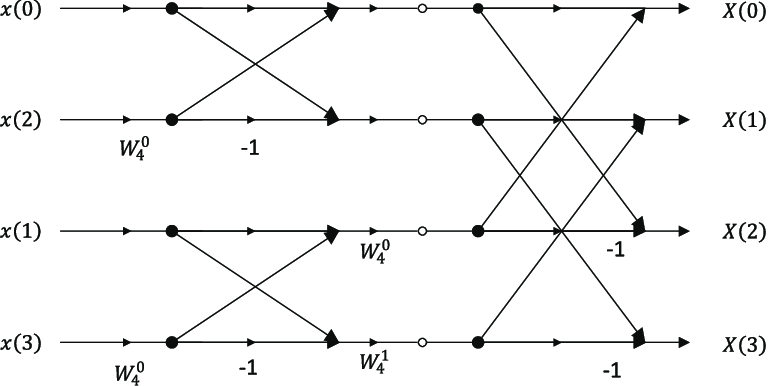
\includegraphics[width=\textwidth]{figures/Length-4-DIT-radix-2-FFT.png}
    \caption{Decimácia v čase}
    \label{fig:dit-fft}
\end{subfigure}
\hfill
\begin{subfigure}[b]{0.48\textwidth}
    \centering
    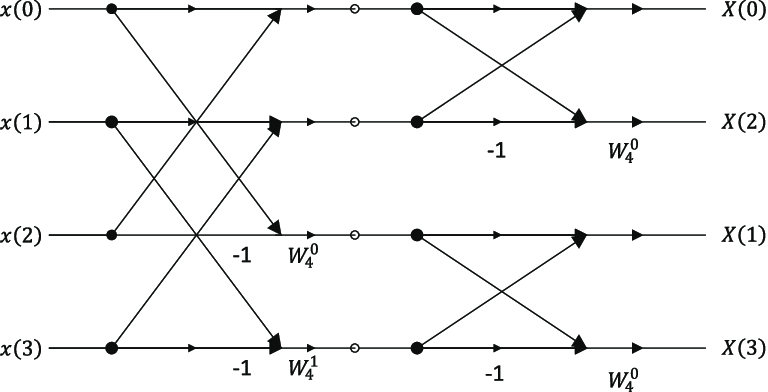
\includegraphics[width=\textwidth]{figures/Length-4-DIF-radix-2-FFT.png}
    \caption{Decimácia vo frekvencii}
    \label{fig:dif-fft}
\end{subfigure}
\caption{Radix-2 FFT na štyroch bodoch \cite{dit-dif-fft}}
\end{figure}

Základným prvkom schémy výpočtu je motýlikový diagram (,,butterfly''), ktorý je odlišný pre DIT (obr. \ref{fig:dit-butterfly})
a pre DIF verziu (obr. \ref{fig:dif-butterfly}). Motýlik obsahuje vynásobenie
jedného z príchodzích operandov s vopred vypočítaným exponenciálnym členom $W_N^j$ pre $j = 0, ..., N/2 - 1$
\cite{fft-blackbox}, a následné prirátanie a tiež odpočítanie od druhého operandu.

\begin{figure}[h]
\centering
\begin{subfigure}[b]{0.48\textwidth}
    \centering
    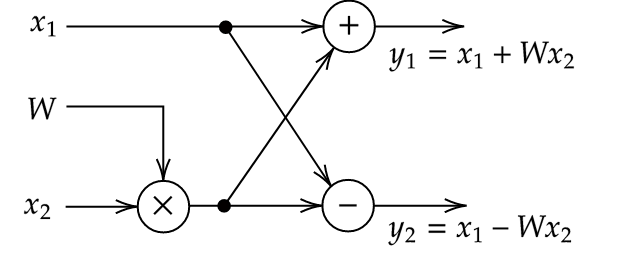
\includegraphics[width=\textwidth]{figures/dit-butterfly.png}
    \caption{Decimácia v čase}
    \label{fig:dit-butterfly}
\end{subfigure}
\hfill
\begin{subfigure}[b]{0.48\textwidth}
    \centering
    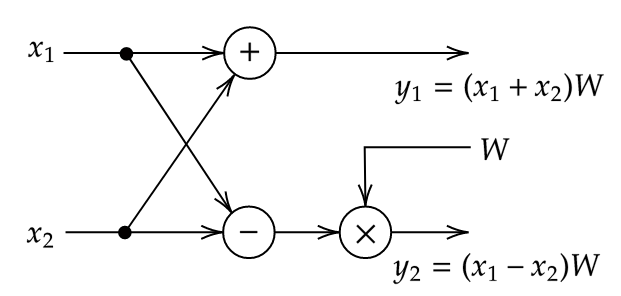
\includegraphics[width=\textwidth]{figures/dif-butterfly.png}
    \caption{Decimácia vo frekvencii}
    \label{fig:dif-butterfly}
\end{subfigure}
\caption{Motýlikové diagramy algoritmu FFT}
\end{figure}

Efektívnejšie na celkový počet aritmetický počet operácií oproti FFT s radixom 2 je \emph{split-radix}, ktorý
kombinuje výhody vyplývajúce z radix-4 pre nepárne členy DFT a radix-2 pre párne členy. Veľkosť vstupného
vektora musí byť násobkom štyroch. Dosahuje okolo 30\% zníženie počtu násobení a 10\% pokles počtu sčítaní
oproti radix-2 \cite{split-radix}.

Algoritmus FFT je aplikovateľný taktiež na výpočet DCT vhodným zoradením vstupného vektora. DCT-II $N$-bodovej
reálnej postupnosti $\mathbf{x}$ sa odvodzuje uskutočnením jej $2N$-bodového párneho rozšírenia a vynásobenie výsledku
twiddle faktorom $2W_{2N}^{k}$ a ponechaní reálnej časti. Na ilustráciu uvádzame prípad
DCT 4-bodovej sekvencie $(x_1, x_2, x_3, x_4)$, ktorej párnym rozšírením $\mathbf{y}$ je $(x_1, x_2, x_3, x_4, x_4, x_3, x_2, x_1)$.
Rovnako by postačovalo vyplniť pôvodnú postupnosť nulami do dĺžky $2N$, čiže dostávame $(x_1, x_2, x_3, x_4, 0, 0, 0, 0)$.
Postačuje však realizovať $N$-bodovú FFT sekvencie párnych alebo nepárnych prvkov z $\mathbf{y}$, ktoré sú vzájomným reverzom.
Na základe predošlého predošlého príkladu dostaneme postupnosť $(x_1, x_3, x_4, x_2)$ \cite{fast-dct}.

Široké použitie FFT pri spracovaní signálov sa prejavuje dostupnosťou implementácií rôznych obmien algoritmu
v širokej škále programovacích jazykov a optimalizované pre konkrétne hardvérové platformy. V jazyku C stoja
za zmienku knižnice: FFTW, FFTPACK, GNU Scientific Library, CMSIS DSP a Espressif DSP. Na účely analýzy údajov je FFT
prítomné pre jazyk Python v balíkoch \emph{numpy} a \emph{scipy}, tiež napr. v jazyku R je súčasťou \emph{stats} modulu.

\subsection{Oknové funkcie}
U stochastického signálu má zmysel delenie na rovnako dlhé úseky, pretože sa s časom mení jeho spektrálny obsah, ktorý
je žiaduce zachytiť čo najpresnejšie. Krátkodobá Fourierová transformácia zahŕňa preto ováhovanie meraní
v časovej doméne koeficientmi posuvnej oknovej funkcie. Mimo intervalu pôsobnosti okna sú vzorky vynulované.

DFT predpokladá periodicitu časového radu do nekonečna, preto ak frekvencia sínusového vstupu nie je presným násobkom
frekvenčného rozlíšenia, čiže priebeh exaktne nepripadá frekvenčnému vedierku, dochádza k úniku spektra (spectral leakage).
Prejavom je hraničný efekt pre odlišnosť poslednej a prvej vzorky, ktorá je považovaná za nespojitosť a prejavuje
sa zvlnením v okolí diskontinuity podľa Gibsovho javu \cite{understanding-dsp}.

Existuje množstvo oknových funkcií líšiacich sa mierou kompromisu medzi šírkou výsledných špičiek vo frekvenčnej doméne,
presnosti v amplitúde a spôsobu poklesu úniku spektra do ostatných vedierok. Medzi najpoužívanejšie sa zaraďujú: obdĺžníkové
(\ref{equ:window-rectangular}), Bartlettovo (\ref{equ:window-bartlett}), Hannovo (\ref{equ:window-hann}), Hammingovo
(\ref{equ:window-hamming}) a Blackmannovo okno \ref{equ:window-blackmann}. Uvedené okná sú stredovo súmerné (obr. \ref{fig:window-time})
Plochejšie okná, napríklad obdĺžníkové, sa vyznačujú ponechaním ostrejších špičiek s neskreslenou amplitúdou za
cenu väčšieho spektrálneho úniku, čím sa znižuje odstup od šumu. Predchádzanie hraničným javom sa dosahuje plynulým
znižovaním hodnôt k okrajom okna až na nulu, čím špičky strácajú na amplitúde (scalloping loss) \cite{spectral-density-estimation}.
\myequations{Oknové funkcie: obdĺžník, Bartlett, Hann, Hamming, Blackman}
\begin{ceqn}\begin{align}
w(n) &= 1,\, n = 0, 1, ..., N - 1 \label{equ:window-rectangular} \\
w(n) &= \frac{2}{N - 1}\left(\frac{N - 1}{2} - \left|n - \frac{N - 1}{2} \right|\right) \label{equ:window-bartlett}  \\
w(n) &= \cos^2((2\pi n / N - \pi) / N)  \label{equ:window-hann} \\
w(n) &= 0.54 - 0.46\cos(2\pi n / N) \label{equ:window-hamming} \\
w(n) &= 0.42 - 0.5\cos(2\pi n / N) + 0.08\cos(4\pi n / N)\label{equ:window-blackmann}
\end{align}\end{ceqn}

Fourierou transformáciou okna dostávame frekvenčnú odozvu, ktorá má tvar funkcie $\mathrm{sinc}(x) = \sin(x) / x$
(obr. \ref{fig:window-freq}) Priebeh odozvy sa vyznačuje hlavným a vedľajšími vrcholmi (mainlobe a sidelobes).
Hlavný vrchol sa snažia
rôzne oknové funkcie udržať čo najužší, lebo zodpovedá za šírku spektrálneho úniku do okolitých vedierok.
Vedľajšie vrcholy sú nežiaduce a podmieňujú najmä úroveň odstupu od šumu.

\begin{figure}[h]
\centering
\begin{subfigure}[b]{0.48\textwidth}
    \centering
    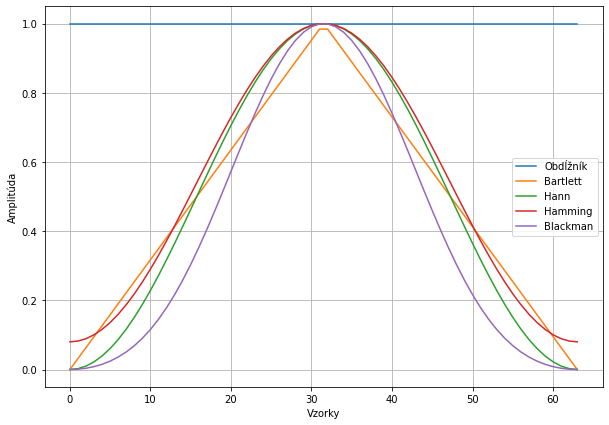
\includegraphics[width=\textwidth]{figures/window-time.png}
    \caption{Časový priebeh}
    \label{fig:window-time}
\end{subfigure}
\hfill
\begin{subfigure}[b]{0.48\textwidth}
    \centering
    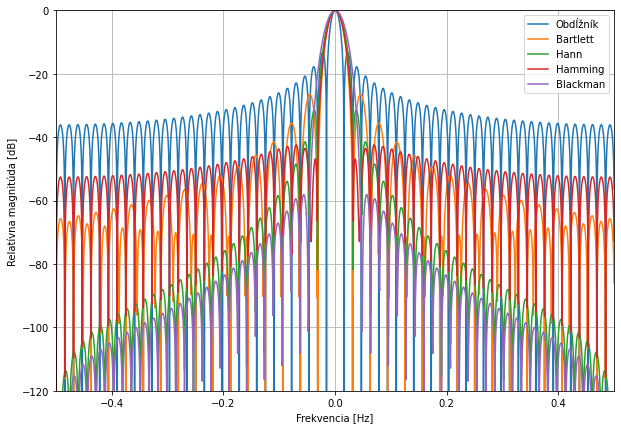
\includegraphics[width=\textwidth]{figures/window-freq.png}
    \caption{Frekvenčná odozva}
    \label{fig:window-freq}
\end{subfigure}
\caption{Tvar oknových funkcií s dĺžkou $N = 31$}
\end{figure}

Vzhľadom na skutočnosť, že oknové funkcie sa typicky blížia nule smerom k okrajom, bola by veľká časť pozorovaní
časového radu ignorovaná. Prekrývaním okien vo vhodnom pomere je umožnený rovnomerný vplyv
hodnôt, ktoré pripadnú na okraj niektorého okna. Pomer sa stanovuje štandardne
na 50\%, aj s ohľadom na rastúcu výpočtovú záťaž s väčším prekrývaním. Výnimkou je obdĺžníkové okno kde to nemá
zmysel. Platí, že pri iných užších oknách je potrebné rátať s väčším presahovaním ako pri širších. Vyhodnotenie veľkosti
prekrývania sa zakladá na korelácii spektrogramov a plochosti amplitúdy, čiže pomeru minimálnej váhy na pozorovanie
vo všetkých oknách ku maximálnej dosiahnutej amplitúde ideálne rovnajúce sa jednotke \cite{spectral-density-estimation}.

Jediný odhad frekvenčných zložiek postupnosti vzoriek vedie k vysokej neurčitosti odhadov pre frekvenčné vedierka,
keďže smerodajná odchýlka odhadu je totožná s odhadom samotným \cite{spectral-density-estimation}. Welchova metóda
spriemerovania upravených periodogramov spresní úrovne frekvencií cez priemer viacerých prekrývajúcich
sa energetických spektier \cite{welch-method}.

\subsection{Filtre s konečnou impulznou odozvou}
Predspracovanie signálu do podoby vhodnejšej na analýzu, extrakciu čŕt a detekciu udalostí sa vykonáva filtrovaním.
Častými činnosťami býva odstránenie posunu alebo jednosmernej zložky, eliminovanie šumu rozptýleného medzi
vysokofrekvenčné komponenty, a oddelenie známeho frekvenčného pásma od zvyšku spektra. Dolná priepusť prepustí
nízke frekvencie až po medznú frekvencie, od ktorej nahor frekvencie utlmuje. Horná priepusť sa správa opačne
a potláča nižšie frekvencie. Pásmová priepusť ponechá frekvencie v obmedzenom rozsahu z oboch strán.

Ideálne filtre majú okamžitý útlm dovoľujúci prechod striktne vymedzeným zložkám signálu. Vo frekvenčnej doméne
oblasti nadobúdajú preto tvar obdĺžníkového okna. Transformáciou do časovej domény sa obdĺžník zmení
na konvolučnú masku, resp. impulznú odozvu $h[k]$, s priebehom $\mathrm{sinc}$ funkcie, ktorá nie je vyjadriteľná nekonečne
presne, čím vznikajú prechodové javy vo frekvenčnej odozve filtra a menšia strmosť útlmu s kratším filtrom.

Konečná impulzná odozva v názve FIR filtra znamená, že pri vyjadrení filtra sa obmedzíme na konečný počet
koeficientov orezaním impulznej odozvy rovného rádu filtra $k$. Výpočet upravenej hodnoty sa v časovej doméne počíta
ako diskrétna konvolúcia s časovou zložitosťou $\mathcal{O}(nk)$, pre časový rad dĺžky $n$. Diagram výpočtu je zachytený
na obr. \ref{fig:fir-filter}.
\myequations{Výpočet FIR filtra cez konvolúciu}
\begin{ceqn}\begin{align}
y[n] = x[n] * h[n] = \sum_{i=0}^{K}{h[i] \cdot x[n - i]}
\end{align}\end{ceqn}

Masky dolnej (\ref{equ:low-pass}), hornej (\ref{equ:high-pass}) a pásmovej priepuste (\ref{equ:band-pass}) popisujú
uvedené vzťahy pre medznú normalizovanú frekvenciu $f_c = f / f_s$ a $n = -k/2, \dots, 0, \dots, k/2$. Zvlnenie v prechodovom pásme
medzi rozsahmi so ziskom a útlmom je vylepšené návrhom filtra za použitia oknovej funkcie (napr. Blackman) na žiadanú
frekvenčnú odozvu.
\myequations{Koeficienty FIR filtra pre dolnú, hornú a pásmovú priepusť}
\begin{ceqn}\begin{align}
h_{LPF}[n] &= \mathrm{sinc}(2 f_c n)  \label{equ:low-pass} \\
h_{HPF}[n] &= (-1)^n \cdot h_{LPF}[n] \label{equ:high-pass} \\
h_{BPF}[n] &= \mathrm{sinc}(2 f_{c2} n) -  \mathrm{sinc}(2 f_{c1} n)  \label{equ:band-pass}
\end{align}\end{ceqn}

Podľa konvolučnej vety platí, že konvolúcia v čase je násobením vo frekvenciách, umožňujúc urýchlenie filtrovania
pre veľké masky. Kým vtedy sa blíži zložitosť konvolúcie ku kvadratickej, na násobenie vo frekvenčnej doméne so
stačí vykonať FFT a IFFT dohromady v rádovo $\mathcal{O}(n \log n)$.

\begin{figure}[h]
	\centering
	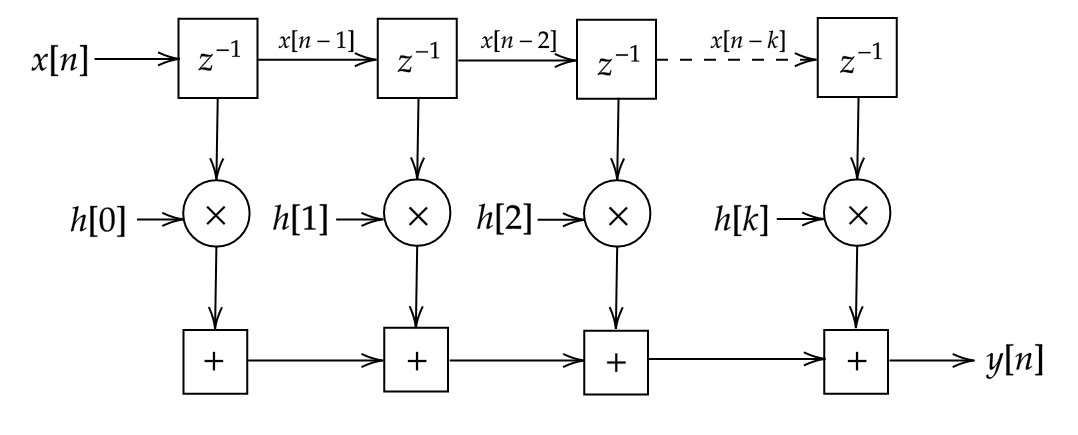
\includegraphics[width=0.8\textwidth]{figures/fir-filter.png}
	\caption{Bloková schéma FIR filtra rádu $k$}
	\label{fig:fir-filter}
\end{figure}

\section{Senzorová sieť}
Zber údajov meraní z prostredia zabezpečujú samočinné senzorové jednotky schopné dlhodobej prevádzky
často za vystavenia nepriaznivým okolitým podmienkam. Hlavnou limitáciou prevádzky senzoriky je spotreba energie,
pretože doba funkčnosti zariadenia ohraničuje kapacita batérií, ktoré sú obtiažne vymeniteľné pri nasadení
v nedostupných lokalitách alebo pozíciach. Senzor musí byť ideálne schopný autonómnej konfigurácie
reakciou na zmenu nastatých okolností a s tým súvisí zotavenie z neočakávaných a chybových stavov \cite{wsn-overview}.

Výpočtový výkon býva za cenu zníženia elektrického odberu redukovaný
znížením taktovacej frekvencie a snahou efektívny manažment periférií distribúciou hodín a dostupnými
úspornými režimami. Menej dostupných cyklov procesora povoľuje realizáciu jednoduchších výpočtov, ktoré zväzuje
u niektorých aplikácií nutnosť odozvy v reálnom čase. Aby sa zachovala nízka cena zariadení šetrí sa
na lokálne dostupnom úložisku, ktoré sa počíta v kilobajtoch nanajvýš megabajtoch.

Senzorové jednotky si buď získané dáta ukladajú na externú flash pamäť, alebo sa od nich vyžaduje komunikácia
cez bezdrôtové spojenie. Prepojením na internet sa zaraďujú k zariadeniam Internetu vecí (IoT).
Na rýchlosť sieťového prenosu má dopad okrem šírky pásma a réžie protokolov
vzdialenosť od sieťovej brány v prípade hviezdicovej topológie alebo najbližšieho susedného uzla v mesh
alebo point-to-point rozložení. Vynaloženým výkonom na príjem a vysielanie je postihnutý dosah, ktorý
ovplyvňujú aj prekážky na trase a iné interferencie. Štandardne používané bezdrôtové technológie
v pásmach ISM sú uvedené v tabuľke \ref{tab:net-protocols}.

\begin{table}[h]
\centering
\def\arraystretch{1.2}
\begin{tabular}{|l|r|rr|r|}
\hline
\textbf{\begin{tabular}[c]{@{}l@{}}Bezdrôtový\\ protokol\end{tabular}} & \multicolumn{1}{l|}{\textbf{\begin{tabular}[c]{@{}l@{}}Frekvenčné\\ pásmo v EÚ\end{tabular}}} & \multicolumn{1}{l|}{\textbf{\begin{tabular}[c]{@{}l@{}}Prenos\\ max.\\ (Mbit/s)\end{tabular}}} & \multicolumn{1}{l|}{\textbf{\begin{tabular}[c]{@{}l@{}}Prenos\\ typ.\\ (Mbit/s)\end{tabular}}} & \multicolumn{1}{l|}{\textbf{\begin{tabular}[c]{@{}l@{}}Dosah\\ cca\\ (m)\end{tabular}}} \\ \hline
Bluetooth LE 4                                                                   & 2,4 GHz                                                                                       & \multicolumn{1}{r|}{1}                                                                         & 0,3                                                                                            & 10 - 30                                                                                 \\ \hline
Bluetooth LE 5                                                                   & 2,4 GHz                                                                                       & \multicolumn{1}{r|}{2}                                                                         & 1,3                                                                                            & 30 - 50                                                                                 \\ \hline
Wifi: 803.11 b                                                                   & 2,4 GHz                                                                                       & \multicolumn{1}{r|}{11}                                                                        & 5                                                                                              & 35 - 140                                                                                \\ \hline
Wifi: 803.11 n                                                                   & 2,4 GHz                                                                                       & \multicolumn{1}{r|}{54}                                                                        & 25                                                                                             & 35 - 140                                                                                \\ \hline
Wifi: 803.11 g                                                                  & 2,4 / 5 GHz                                                                                   & \multicolumn{1}{r|}{300 / 600}                                                                 & 150                                                                                            & 70 - 250                                                                                \\ \hline
ZigBee: 802.15.4                                                                 & \begin{tabular}[c]{@{}r@{}}868 MHz\\ 2,4 GHz\end{tabular}                                     & \multicolumn{2}{r|}{\begin{tabular}[c]{@{}r@{}}20 kbit/s\\ 250 kbit/s\end{tabular}}                                                                                                             & 10 - 100                                                                                \\ \hline
Z-Wave                                                                           & 868 MHz                                                                                       & \multicolumn{2}{r|}{40 - 100 kbit/s}                                                                                                                                                            & 30 - 100                                                                                \\ \hline
LoRaWAN                                                                          & 863 MHz                                                                                       & \multicolumn{2}{r|}{0,3 - 50 kbit/s}                                                                                                                                                            & 5 - 20 km                                                                               \\ \hline
Narrowband IoT                                                                   & \multicolumn{1}{l|}{Operátor}                                                                 & \multicolumn{2}{r|}{250 kbit/s}                                                                                                                                                                 & \multicolumn{1}{l|}{1 - 10 km}                                                          \\ \hline
\end{tabular}
\caption{Prehľad najpoužívanejších typov sietí pri IoT komunikácii}
\label{tab:net-protocols}
\end{table}

Na harmonizáciu využívania rádiového frekvenčného spektra pre zariadenia s krátkym dosahom sa v
Slovenskej republike vzťahuje vykonávacie rozhodnutie Komisie Európskej únie 2019/1345. Definujú sa
tam voľné frekvenčné pásma s povoľovaním príslušného maximálneho legálneho vysielacieho výkonu
zariadení \cite{eu-frequencies}.

V Sub-1 GHz oblasti je k dispozícii rozsah 863 - 870 MHz využívaný LPWAN (Low-Power Wide Area Network) obmedzený
časom vysielania na 0.1\%, 1\%, alebo 10\% z hodiny a výkonom do 25 mW. Wifi (IEEE 803.11) a Bluetooth zaberajú
rozsah 2400 - 2 483,5 MHz s povoleným výkonom do 100 mW na 100 KHz. Protokoly
ako Bluetooth sa navyše označujú triedami podľa ponúkaného dosahu. Trieda 1 deklaruje dosah do 100 metrov za výkonu
do 100 mW, trieda 2 je približne do 10 metrov a do 2,5 mW a trieda 3 je na 1 meter a 1 mW \cite{bluetooth}.
IoT tiež využíva na komunikáciu mobilné siete poskytované operátormi (napr. NB-IoT, GPRS, 3G, 4G/LTE a 5G),
tam sú frekvencie licencované.

Operácia uzlov sa rozdeľuje podľa podnecujúceho činiteľa ako založené na udalostiach (event-driven),
dopytoch (query-driven) alebo čase (time-driven) \cite{big-data-collection-wsn}. Event-driven
nepretržite vyhodnocuje vstupy ale upozorní až po zachytení náhlej zmeny alebo prekročení prahovej úrovne.
Query-driven systém reaguje na aktuálne požiadavky od používateľa a odpovie so sadou dát zodpovedajúcej požiadavke.
Time-driven systém pravidelne odosiela zozbierané údaje do siete podľa nastavení od riadiaceho uzla.

IoT zariadenia na okrajoch siete vytvárajú veľký objem dát, ktorý sa tradične posiela na zhromaždenie, spracovanie
a analýzu na centrálny server alebo do cloudu. Posunom paradigmy s cieľom vyhodnotenia dát, čo najbližšie
ku zdroju dát za zníženia latencie pri spracovaní, sieťovej premávky a záťaže na cloudové riešenie, a zvýšením
bezpečnosti sa rozširuje edge computing (,,počítanie na okraji'').
\begin{figure}[h]
	\centering
	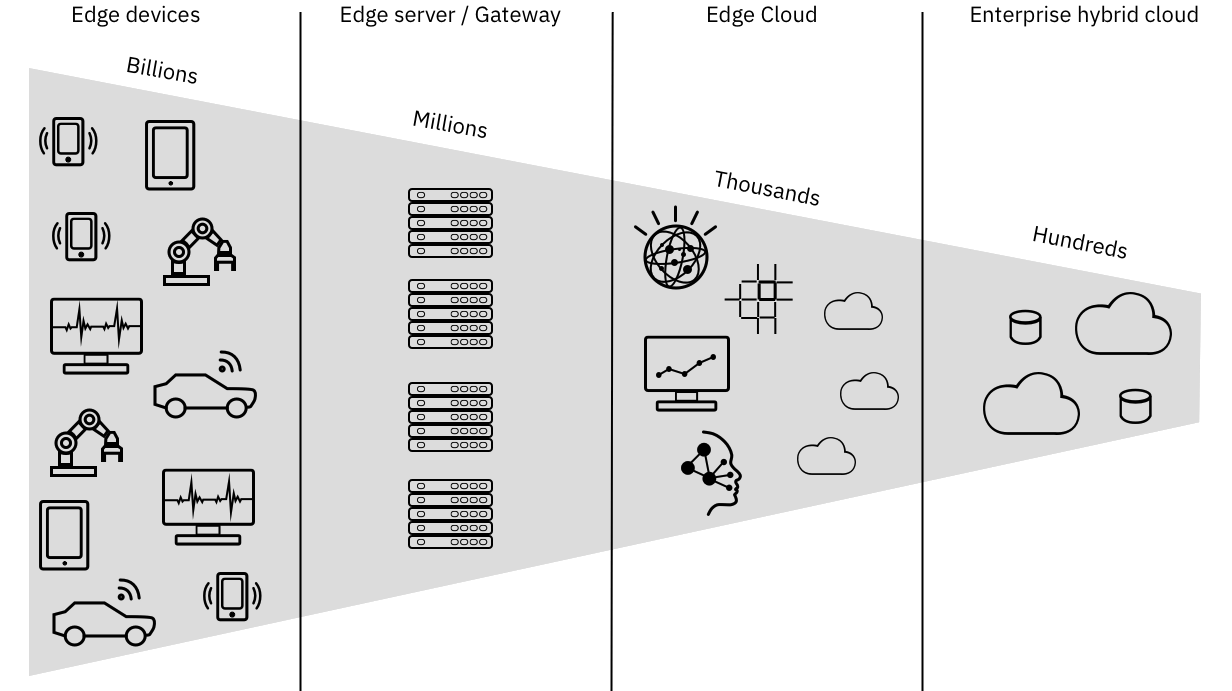
\includegraphics[width=0.9\textwidth]{figures/edge-computing.png}
	\caption{Prvky architektúry Edge computing \cite{ibm-edge-architecture}}
	\label{fig:fir-filter}
\end{figure}

Edge computing je viacvrstvová distribuovaná architektúra vyvažujúca zodpovednosti a záťaž medzi
tri vzájomne sa dopĺňajúce úrovne: Device edge, Local edge a Cloud \cite{edge-computing-survey}. Na okraji sieti
vrámci device edge pôsobia  samotné IoT zariadenia získavajúce dáta z fyzických veličín prostredia a posielajú ich
sieťovým edge bránam. Local Edge zahŕňa aktívne sieťové prvky a aplikácie s úlohami, ktoré nie je možné realizovať
okrajovými zariadeniami. V cloude sa zhromažďujú dáta do dlhodobého úložiska pre komplexnú a celistvú analytiku.
Zároveň cloud obsahuje softvér na spravovanie a monitorovanie zdrojov.



\chapter{Opis riešenia}
Požiadavky
\begin{itemize}
\item Najvhodnejší spôsob identifikácie lokálnych extrémov - špičiek
\item Možnosti redukcie zberu dát za cenu redukcie energetické nároky a prenosu významných čŕt signálu
\item Pravidlový systém na definíciu udalostí záujmu operátorov a ich spoľahlivá identifikácia
\item Upozornenie na nezvyčajnosti pri prevoze (detekciou anomálií) - veľká nerovnosť, neočakávaný pohyb
\end{itemize}

Senzorová jednotka s akcelerometrom na meranie vibrácii a nárazov pri prevoze krehkých látok/materiálov upozorňujúca na základe konfigurovateľných pravidiel alebo nezvyčajných vzorov (pozn.:lepšie dodefinovať). Preskúmanie možností redukcie zberu alebo nasnímaných údajov - nastavenie vzorkovacej frekvencie / akceptovanie nad stanovenú amplitúdu / kompresia. Rozšírenie: /distribuovaná/ korelácia údajov z viacerých akcelometrov z jedného balíka / vozidla.

\section{Hardvér senzorovej jednotky}
\section{Vývojové prostredie a knižnice}
CMSIS, MDK5, OPENOCD, GCC
\section{Koordinácia subsystémov}
\section{Konzervácia energie znížením vzorkovania}
\section{Pravidlový systém na extrahovanie čŕt záujmu}


Táto časť bakalárskeho projektu obsahuje opis výsledkov riešenia jednotlivých etáp projektu. V prípade, že záverečný projekt nerieši všetky etapy, malo by byť v príslušnej časti uvedené kto, resp. kde sa príslušná etapa rieši/riešila/bude riešiť.

Typické etapy riešenia pri tvorbe softvérového systému:
\begin{itemize}
    \item špecifikácia požiadaviek
    \item návrh
    \item implementácia (ak to zadanie požaduje)
    \item overenie riešenia
\end{itemize}

Podľa možností treba vychádzať zo známych prístupov (napr. pri softvérových projektoch štruktúrovaný alebo objektovo orientovaný prístup) a techník (napr. blokové schémy, vývojové diagramy, UML, entito-relačné diagramy atď.). Táto časť práce závisí od konkrétneho zadania.
Je dôležité prezentovať návrhové rozhodnutia, alternatívy, ktoré sa zvažovali pri riešení a samotný návrh riešenia zadaného problému. Štruktúrovanie textu tejto časti BP by malo vychádzať zo zadanej úlohy, ktorá sa rieši. Najmä v tejto časti študent preukazuje tvorivý prístup k riešeniu problémov a kritické myslenie.
\emptypage 


\chapter{Implementácia} \label{chapter:implementation}
Firmvér senzorovej jednotky je implementovaný v programovacom jazyku C so
SDK Espressif IoT Development Framework (ESP-IDF). Súbežný beh úloh spravuje operačný systém reálneho času FreeRTOS.
Optimalizované rutiny spracovania signálu poskytuje Espressif DSP Library. Knižnica MPack má na starosti
kódovanie a dekódovanie formátu Message Pack. CMake riadi zostavovanie
modulov zdrojového kódu. Eclipse Mosquitto pôsobí ako MQTT broker správ.

V jazyku Python sú napísané Jupyter notebooky na analýzu zozbieraných datasetov a otestovanie fáz navrhnutej dátovej pipeline,
so závislosťami numpy, scipy, pandas a matplotlib. Rozhranie príkazového riadku na nahrávanie konfigurácie a náhľad odoberaných
správ sa spolieha na balíčky Paho MQTT, cmd a msgpack.

\section{Senzorová sieť}
Súčiastky FireBeetle ESP32, OpenLog, STEVAL-MKI159V1 a BTS117 sú naspájkované na univerzálny plošný spoj rozmerov 5 x 7 cm
(obr. \ref{board}). Doska je vsadená do plastovej krabičky s hrúbkou stien 3 mm vo výške 2 cm nad povrchom.
Akcelerometer je namontovaný tesne pod modulom MCU. Externý 5 V zdroj sa pripája cez Micro USB konektor, alebo 3,7 V lítiovú batériu 
zapojíme cez JST PH 2 pin.
\begin{figure}[h!]
\centering
\begin{subfigure}{0.6\textwidth}
    \centering
    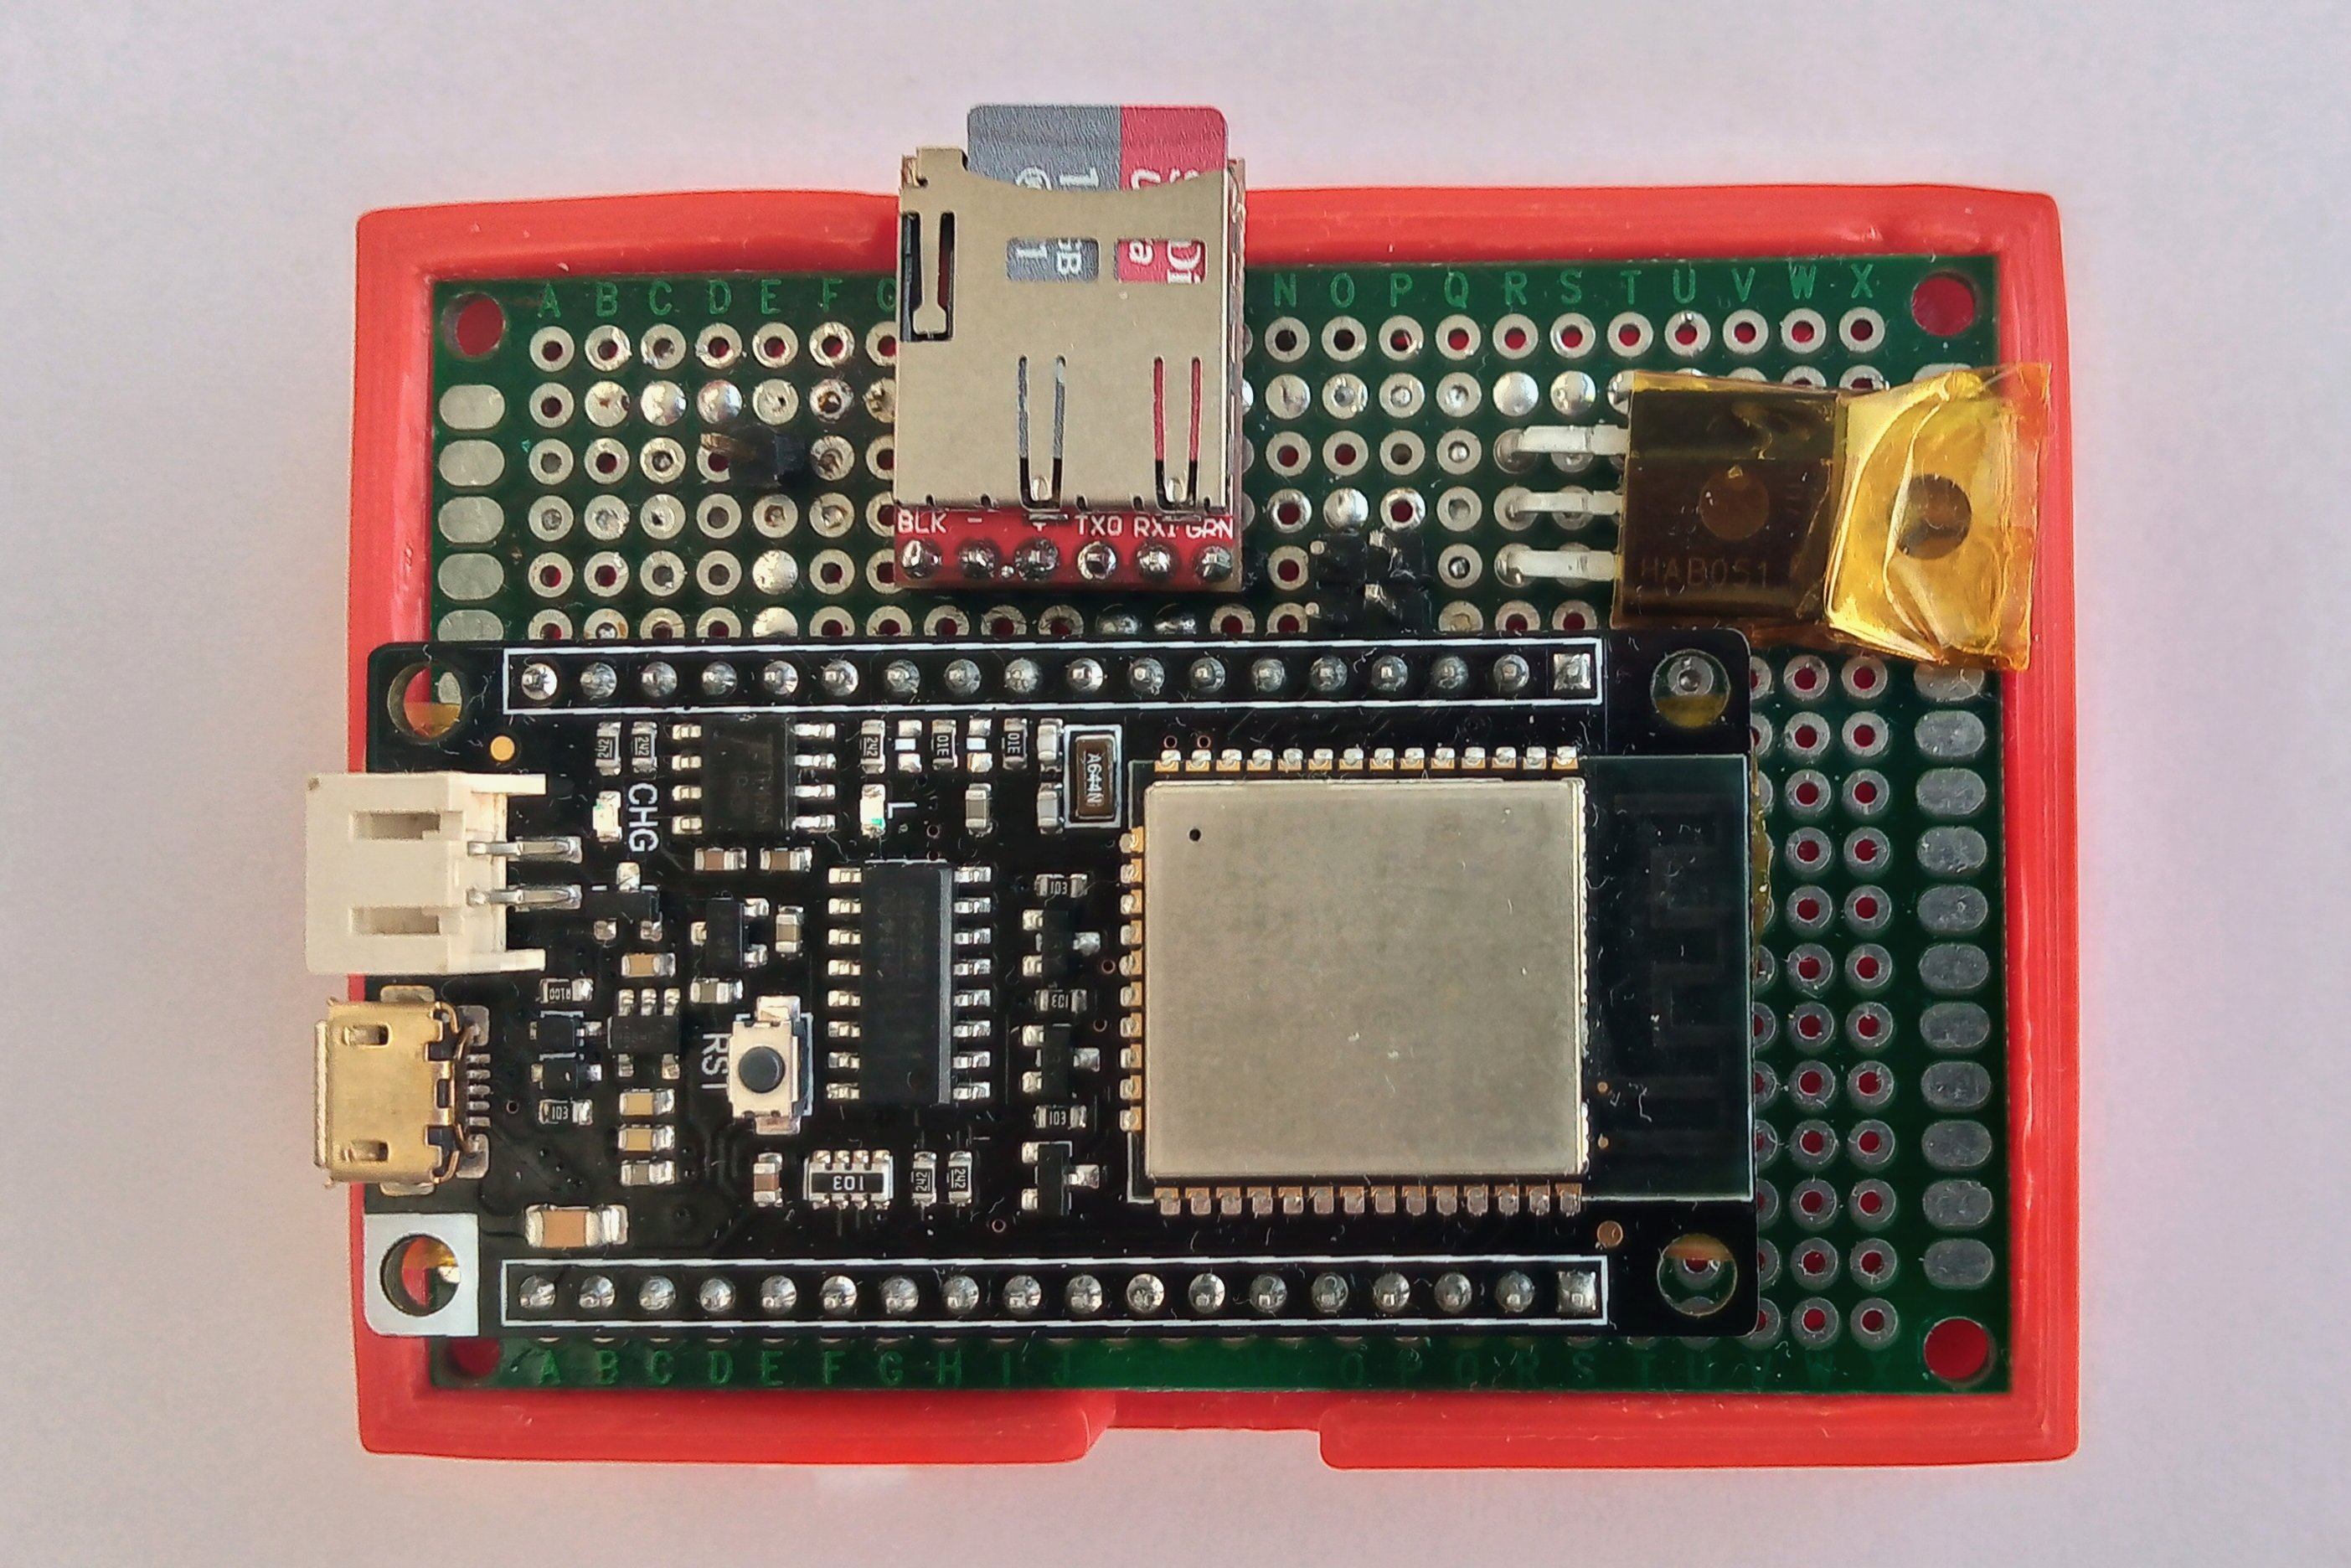
\includegraphics[width=\textwidth]{figures/design/esp32.jpg}
\end{subfigure}
\begin{subfigure}{0.2\textwidth}
    \centering
    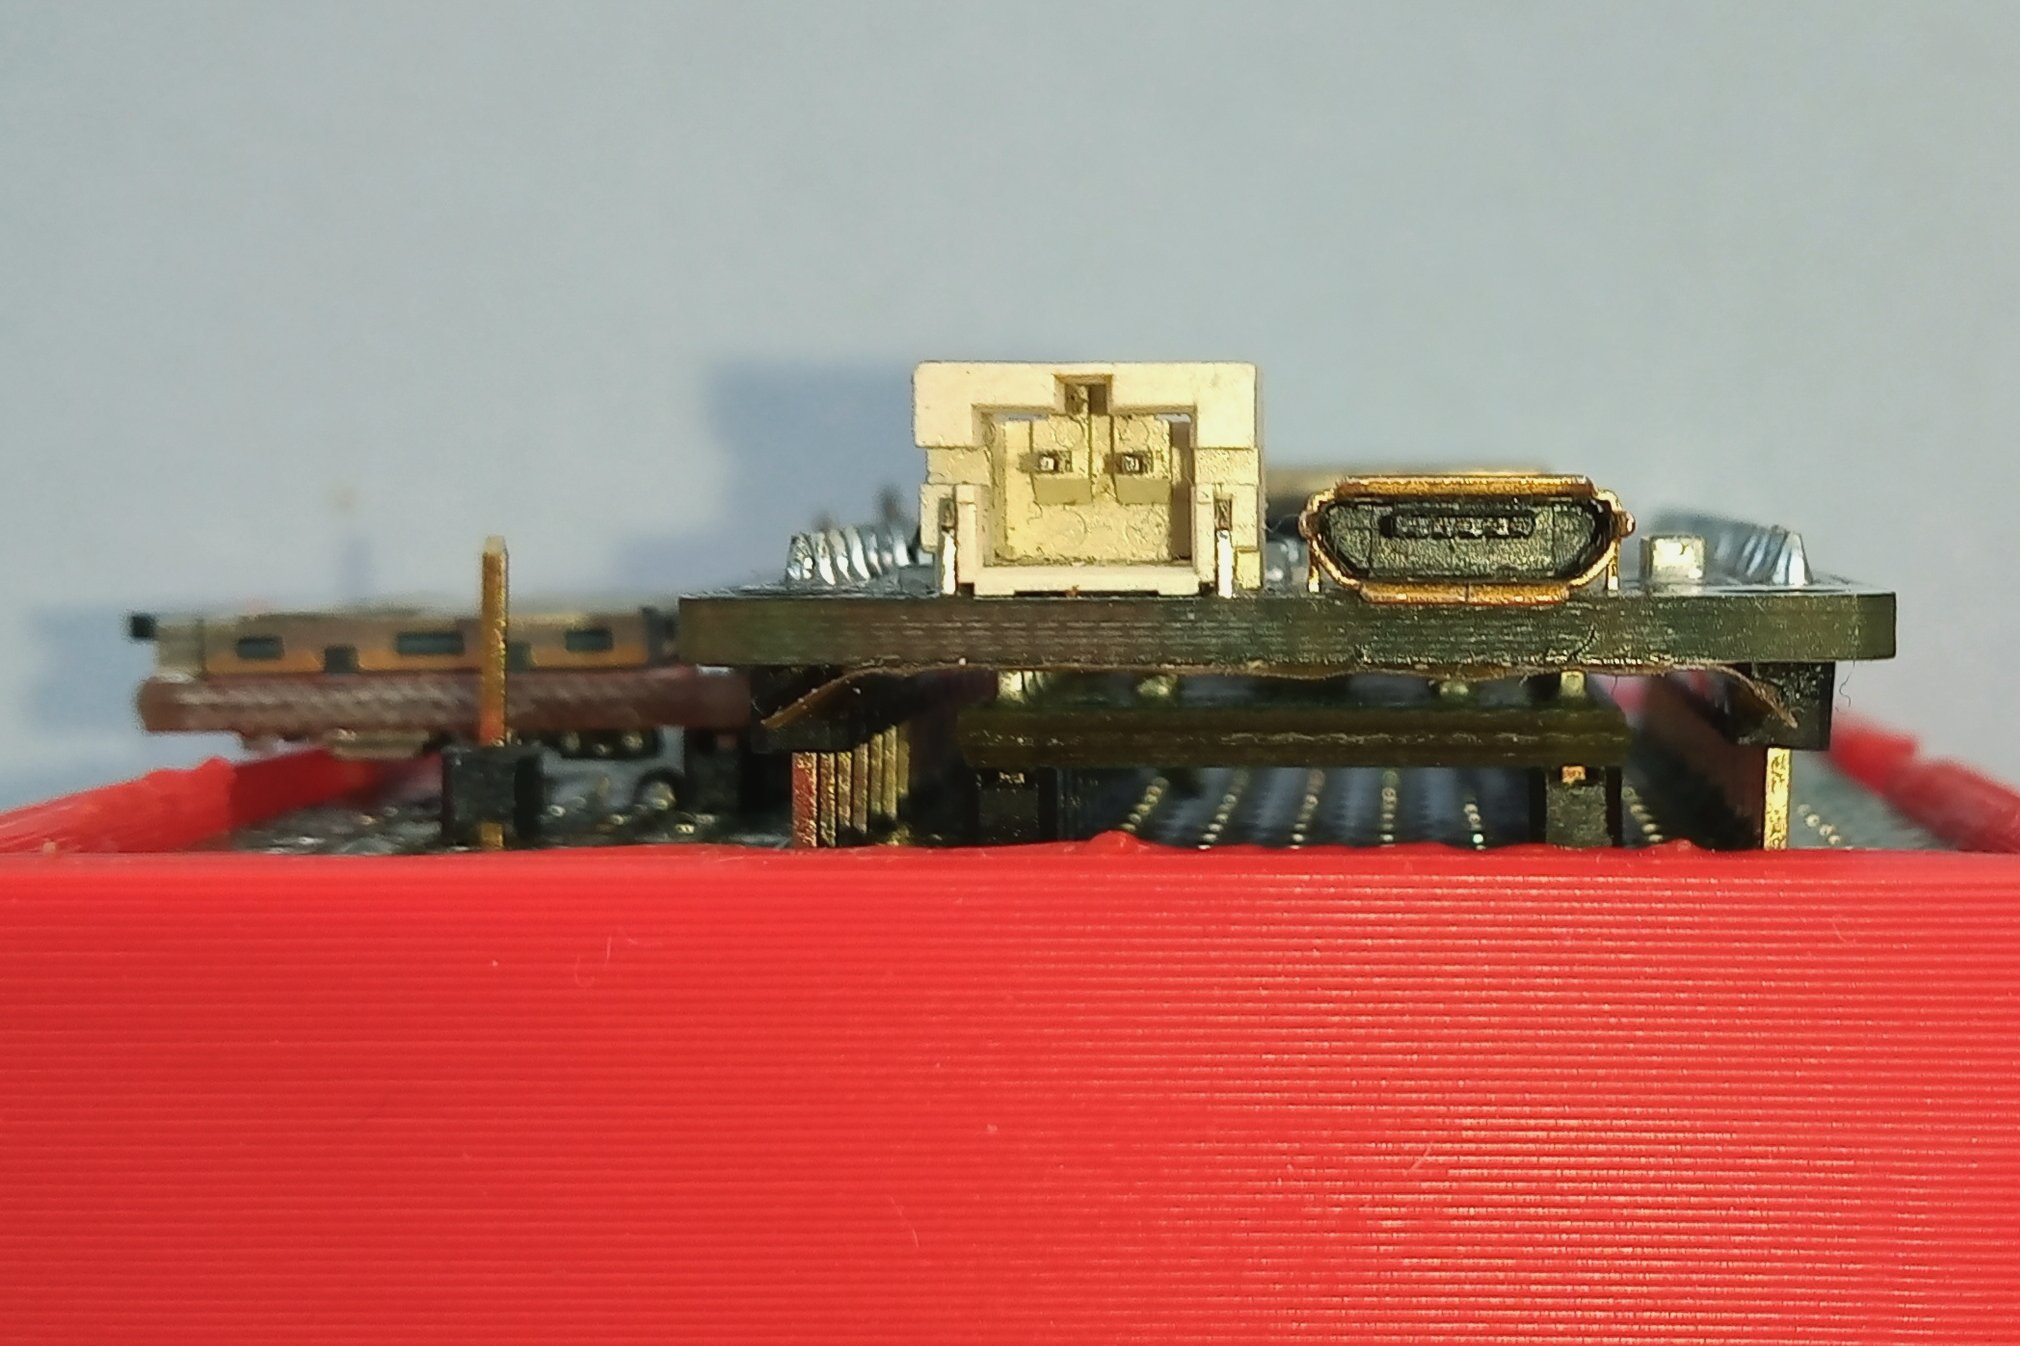
\includegraphics[width=0.9\textwidth]{figures/design/esp32-front.jpg}
\end{subfigure}
\caption{Univerzálny plošný spoj v krabičke osadený modulmi}
\label{board}
\end{figure}

Po zapnutí si firmvér načíta systémové nastavenia cez SDK Storage API z flash. Inicializuje sa
akcelerometer a naraz sa kompletne alokuje dynamická pamäť pre výpočty dátovej pipeline a pre synchronizačné primitíva.
Na zamedzenie fragmentácie nie je odvtedy programom prideľovaná žiadna ďalšia pamäť okrem zásobníkov úloh.

Prebehne pokus o pripojenie s prístupovým bodom WiFi so zabezpečením WPA2 a so serverom MQTT broker, na základe prihlasovacích údajov
a URL adresy v štruktúre \verb|Provisioning|. Proces spustenia OpenLog čaká po zopnutí napájania 10 sekúnd na uvedenie
periférie do prevádzkyschopného stavu.
\begin{lstlisting}[style=implementation]
Provisioning login = {
    .wifi_ssid="AccessPoint",
    .wifi_pass="password",
    .mqtt_url="mqtt://192.168.1.2:1883"
};
\end{lstlisting}

Priame prepísanie predvolenej hodnoty systémového nastavenia v zdrojovom kóde
sa po nahratí firmvéru neprejaví za behu. Predtým sa musí naflashovať obslužný program vyvolaní direktívou
\verb|FACTORY_RESET| pri kompilácii, ktorý premietne tieto nastavenia do partície nevolatilnej pamäte.

Broker MQTT správ Eclipse Mosquitto nasadený v lokálnej sieti, má umožnené cez konfiguračný súbor \verb|mosquitto.conf| počúvať
premávku zo všetkých IP adries na TCP porte 1883, bez nutnosti klientov sa autentifikovať:
\begin{lstlisting}[style=implementation]
listener 1883 0.0.0.0
allow_anonymous true
\end{lstlisting}

Vlastný MQTT klient \verb|config_tool.py| je interpreter príkazov na interaktívnu interakciu so senzorovými jednotkami
pripojenými na broker. Ponúka nadstavbu nad binárnymi správami v Message Pack konverziou z a do ľudsky čitateľnejšej
podoby vo formáte JSON. Povelom \emph{connect} dôjde k nadviazaniu spojenia s brokerom správ, za filtrovania topics podľa
zadaného identifikátora zariadenia. Prefix MQTT tém definuje konštanta firmvéru \verb|DEVICE_MQTT_TOPIC|, ktorý konvenčne začína
s ,,imu/[Device ID]/''.

Režim na nastavenie systémovej konfigurácie IoT koncového uzla sa vyvolá povelom \verb|set| a dopyt aktuálnych pravidiel
príkazom \verb|config|. Po aplikovaní zmien sa čaká sa opätované nabehnutie systému alebo chybovú hlášku.
Zobrazenie jednotkou publikovaných údajov na MQTT tému alebo skupinu tému sa určuje povelom \verb|topic|.

Na SD karte data loggera sa nachádza súbor \verb|config.txt| s uvedenou znakovou rýchlosťou
rovnakou ako pre UART zbernicu mikrokontoléra. Preferované nastavenia sú najvyššia prenosová rýchlosť 115000
v móde 0 zakladajúcom nový log súbor po reštarte:
\begin{lstlisting}[style=implementation]
115200,36,3,0,1,1,0
baud,escape,esc#,mode,verb,echo,ignoreRX
\end{lstlisting}

\section{Komunikácia medzi úlohami}
Nezávislé činnosti aplikácie sú prerozdelené medzi vlákna, ktoré si cez fronty posielajú súradnice zrýchlenia.
FreeRTOS úlohy sú funkcie vykonávajúce opakované sekvenciu príkazov v nekonečnom cykle.

Procedúra obsluhy prerušenia hardvérového časovača nesmie čakať, preto je načítaná rovno z IRAM a upovedomí úlohu vzorkovania
(kód \ref{lst:sampling}). Prevzatím notifikácie synchrónne pošle riadiace slovo senzoru na sekvenčné odčítanie celého vektora
akcelerácie od bázovej adresy registra x-ovej osi. Získaná trojica 16-bitových slov sa podľa aktuálneho rozlíšenia prevedie
do štandardnej fyzikálnej jednotky v type \verb|float|.

\begin{lstlisting}[style=cstyle,caption=Posielanie vzoriek medzi úlohami cez fronty,label={lst:sampling},
 morekeywords={ulTaskNotifyTake,xQueueSend,xQueueReceive,buffer_shift_left,p.stream}]
// Sampling task
if (ulTaskNotifyTake(pdTRUE, portMAX_DELAY)) {
	imu_acceleration(&imu, &axis[0], &axis[1], &axis[2]);
	for (i = 0; i < AXIS_COUNT; i++) {
    	if (conf.sensor.axis[i])
        	xQueueSend(pipeline.queue[i], &axis[i], 0);
    }
}
// Pipeline task
if (xQueueReceive(k->queue[x], &p.stream[idx], portMAX_DELAY)) {
	if (++idx < conf.sensor.n) continue;
    // Process buffer p.stream
    buffer_shift_left(p.stream, conf.sensor.n, leftover);
    idx = conf.sensor.n - leftover;
}
\end{lstlisting}
Vkladanie vzoriek do fronty neblokuje, lebo sa nepočíta s úplným vyčerpaním voľných slotov. Posiela sa do fronty
iba vtedy, ak beží úloha pipeline pre danú dimenziu. Na opačnom konci fronty sa čísla po jednom pripájajú do
cirkulárnej vyrovnávacej pamäte. Pole sa prenechá zvyšku úlohy na spracovanie až po naplnení
dosiahnutím \verb|conf.sensor.n| položiek.

Dokončením analýzy posuvného okna sa presunú ponechané hodnoty z prekryvu časových úsekov na začiatok
poľa: $\mathrm{leftover} = n \cdot (1 - \mathrm{overlap})$. Ďalej sa pokračuje prepisovaním už nepotrebných čísel od pozície \verb|idx|.

\begin{lstlisting}[style=cstyle,caption=Synchronizácia úloh na výpočet korelácie osí,label={lst:correlation},
morekeywords={xEventGroupSync}]
xEventGroupSync(barrier, (1 << axis), task_mask, portMAX_DELAY);
	float avg = mean(buffer, n);
	std[axis] = sqrt(variance(buffer, n, avg));
	for (uint16_t i = 0; i < n; i++)
		diff[axis][i] = (buffer[i] - avg);
xEventGroupSync(barrier, (1 << axis), task_mask, portMAX_DELAY);

if (axis[0] && axis[1])
   stats->corr_xy = correlation(diff[0],diff[1],n,std[0],std[1]);
\end{lstlisting}

Okrem synchronizácie úloh posielaním správ cez fronty sa zužitkúvajú bariéry. Event Groups riadia toky
synchronizovaných úloh v bodoch stretu čakaním na nastavenie bitov podľa očakávanej bitovej masky. Počas
autorizácie voči prístupovému bodu WiFi čaká podprogram hlavného vlákna na príznak pridelenia IP adresy
od obsluhy udalosti nadviazania spojenia.

Koordinácia vlákien je nevyhnutná tiež pri výpočte korelácie, pretože každá os je spracovaná nezávisle. Proces
prezentuje zjednodušený kód \ref{lst:correlation}.V sekcii medzi bariérami si úlohy predpočítajú smerodajnú odchýlku a zoznam rozdielov
od aritmetického priemeru. Konštanta \verb|task_mask| značí bitovými vlajkami, ktoré osi sú aktivované.
Na základe $\mathrm{axis} \in \{0,1,2\}$ signalizuje konkrétne vlákno, že prišlo ku bariére. Mimo kritickej oblasti
si jednotlivé vlákna, disponujúce medzivýsledkami za každú zložku vektora, dorátajú momentálne povolené
kombinácie dvojíc súradníc individuálne.

\section{Udalosti vo frekvenčnom spektre}
ESP DSP knižnica optimalizuje pre naše účely transformáciu do frekvenčnej domény, algoritmami FFT s radixom 2 alebo DCT-II,
a vyhladenie signálu konvolúciou. Avšak dostupná implementácia kosínusovej transformácie nie je adekvátna.
Vyžaduje štvornásobnú veľkosť tabuľky koeficientov ku veľkosti transformácie a vnútorne volá generický
algoritmus FFT. Prišlo k úprave zdrojového kódu knižnice, aby sa aspoň použila platforme prispôsobená verzia.

Pred oboma typmi transformácii sa vynásobia vzorky v posuvnom okne s pripravenými váhami oknovej funkcie (kód \ref{fft}).
Líši sa spôsob napĺňania vstupného poľa, kde u FFT tvoria reálne čísla na párnom a nepárnom mieste za sebou
spoločné komplexné číslo. DCT ponecháva následnosť reálnych vstupov, zato prázdna druhá polovica poľa zostáva
na pracovné účely funkcie.

Poradie vedierok výsledného spektra FFT sa musí explicitne bitovo invertovať a previesť späť na striedanie
reálnych a imaginárnych zložiek. Na záver sú zistené magnitúdy komplexných čísel.
Prepočet na decibely berie za referenčnú úroveň frekvenciu s najväčšou intenzitou.

\begin{lstlisting}[style=cstyle,label={fft},caption=Fourierová a kosínusová transformácia s ESP DSP knižnicou]
case DFT:
	for (uint16_t i = 0; i < n; i++) {
		spectrum[2*i+0] = buffer[i] * window[i];
		spectrum[2*i+1] = 0;
	}
	dsps_fft2r_fc32_ae32(spectrum, n);
	dsps_bit_rev2r_fc32(spectrum, n);
	dsps_cplx2reC_fc32(spectrum, n);
case DCT:
	for (uint16_t i = 0; i < n; i++)
    	spectrum[i] = buffer[i] * window[i];
    dsps_dct_f32(spectrum, n);
\end{lstlisting}

Stav detektora udalostí pozostáva z poľa štruktúr \ref{event:struct}, ktoré odvádzajú časové značky
počiatku, trvania a naposledy videnej špičky od počítadla prebehnutých posuvných okien. Upozornenie na
zmeny vo frekvencii sa pri prechode prúdovým algoritmom poznačí do vymenovaného typu
aktuálnej akcie \verb|SpectrumEventAction|. Nadobúda konštanty z množiny ,,nič'', ,,štart'' alebo ,,koniec'' a
obnovujú sa na začiatku každého ďalšieho kola, na stav neprítomnosti akejkoľvek zmeny. Udalosti na odoslanie
sú síce pri serializácii správy lineárne prehľadávané, ale vytráca sa potreba udržiavať zásobník emitovaných udalostí.

\begin{lstlisting}[style=cstyle,label={event:struct},
caption={Štruktúra udalosti frekvenčného vedierka},morekeywords={SpectrumEvent}]
typedef struct {
    SpectrumEventAction action;
    uint32_t start;
    uint32_t duration;
    int32_t last_seen;
    float amplitude;
} SpectrumEvent;
\end{lstlisting}

\section{Systémová konfigurácia}
Správanie blokov dátovej pipeline určuje globálna inštancia zloženej štruktúry \emph{Configuration} \ref{config:struct}.
Vnorené členské premenné definujú vlastnosti jednotlivých funkčných blokov. Po zapnutí je posledná
konfigurácia zobraná ako blob z nevolatilnej pamäte pod kľúčom ,,config''. Chýbajúca podpora iných ako celočíselných
typov znamená, že po akejkoľvek úprave musí byť štruktúra znovu nahratá do flash pamäte ako celok.

\begin{lstlisting}[style=cstyle,label={config:struct},caption=Štruktúra systémovej konfigurácie,
morekeywords={Configuration}]
typedef struct {
    SamplingConfig sensor;
    SmoothingConfig tsmooth;
    StatisticsConfig stats;
    FFTTransformConfig transform;
    SmoothingConfig fsmooth;
    EventDetectionConfig peak;
    SaveFormatConfig logger;
} Configuration;
\end{lstlisting}

Názvy, typy a prípustné hodnoty atribútov vo formáte Message Pack sú vyjadrené imperatívne priamo vo funkciách
na konštruovanie a rozklad reťazca dátového obsahu paketu. Parsovanie prebieha v jednom prechode s MPack Expect API
umožnením flexibilného poradia kľúčov, ktoré umožňuje priradiť modifikované pravidlo do kópie štruktúry bez dodatočného
syntaktického stromu.


\chapter{Overenie riešenia}
Funkčnosť a efektivitu riešenia v súlade s kladenými požiadavkami overíme v rozličných scenároch. Zároveň experimentálne
demonštrujeme odvodenie hyperparametrov klasifikácie špičiek s mriežkovým vyhľadávaním (grid search)
a vyjadríme úspešnosť zaužívanými metrikami.

\section{Pamäťová efektivita}
Skompilovaný program senzorovej jednotky sa zmestí do pamäte inštrukcií so značnou rezervou. Kódový segment zaberá
64,42\% alebo 81,8 kB dostupného priestoru vynímajúc vyhradené časti na vektory prerušení a vyrovnávacie pamäte procesora.
Obsadením 43,4 kB v segmente .bss, prevažne na staticky alokované polia reťazcov odosielaných správ, a nárokovania si 14,7 kB
konštánt, zostáva 82,3\% DRAM na haldu. Spotrebu SRAM v bajtoch podľa segmentov objektového súboru podľa nástroja
\emph{GNU size} uvádza tabuľka \ref{tab:ram-segments}.
\begin{table}[h]
\def\arraystretch{1.25}
\begin{tabular}{|l|llll|lll|}
\hline
                     & \multicolumn{4}{c|}{\textbf{IRAM (192 kB)}}                                                                              & \multicolumn{3}{c|}{\textbf{DRAM (328 kB)}}                                           \\ \hline
\textbf{Sekcia}      & \multicolumn{1}{l|}{CPU cache} & \multicolumn{1}{l|}{.vectors} & \multicolumn{1}{l|}{.text} & voľné                      & \multicolumn{1}{l|}{.bss}  & \multicolumn{1}{l|}{.data} & voľné (heap)                \\ \hline
\textbf{Veľkosť (B)} & \multicolumn{1}{r|}{65536}     & \multicolumn{1}{r|}{1027}     & \multicolumn{1}{r|}{83780} & \multicolumn{1}{r|}{46265} & \multicolumn{1}{r|}{44392} & \multicolumn{1}{r|}{15040} & \multicolumn{1}{r|}{276440} \\ \hline
\end{tabular}
\caption{Rozdelenie pamäte medzi sekcie}
\label{tab:ram-segments}
\end{table}

Vyťaženie dynamickej pamäte z haldy lineárne závisí od počtu súčasne vyhodnocovaných údajových bodov. Trend sa prejavuje v grafe
celkovej percentuálnej naplnenosti haldy \ref{graph:mem-usage}. Markantný stály podiel z voľného priestoru až okolo 55 kB sa poskytne na komunikáciu cez WiFi a na TCP/IP protokolový zásobník (graf \ref{graph:task-memory})

Zvyšok sa dá k dispozícii vlákna úloh na manipuláciu so vzorkami osí zrýchlenia (x, y, z), na zdieľané koeficienty FFT a
konvolučné masky a  relatívne nepatrne si obsadia úlohy vzorkovania (imu) a zápisu na pamäťovú kartu (logger).
FreeRTOS je nastavený na dynamickú alokáciu zásobníkov, preto už pri veľkosti okna 8 potrebuje spracovateľská úloha 10 kB. Najdlhšie
akceptovateľné posuvné okno a tým aj veľkosť frekvenčnej transformácie je 1024 bodov, ktoré vzhľadom na 97\% spotreby haldy za istých
okolností vykazuje nestabilitu systému. Odporúča sa pri zložitejšom procese úpravy signálu vystačiť si s 512 bodmi.

\begin{figure}[h]
	\centering
     \hfill
     \begin{subfigure}{0.48\textwidth}
        \centering
     	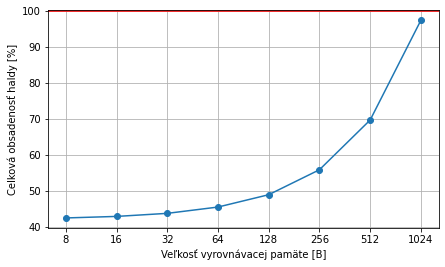
\includegraphics[width=\textwidth]{figures/verification/memory-usage-percentage.png}
     	 \caption{Celková spotreba pamäte}
     	 \label{graph:mem-usage}
     \end{subfigure}
     \hfill
      \begin{subfigure}{0.48\textwidth}
    	\centering
        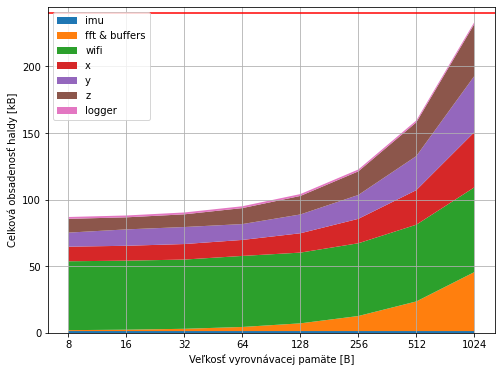
\includegraphics[width=\textwidth]{figures/verification/memory-profile-bytes.png}
         \caption{Rozdelenie pamäte medzi úlohy}
        \label{graph:task-memory}
     \end{subfigure}
     \caption{Profilovanie dynamickej pamäte z haldy v DRAM}
\end{figure}


Veľkosť vyrovnávacej pamäte má priamy dopad na objem posielanej sieťovej premávky, ako vyčísľuje tabuľka \ref{tab:msg-size} v bajtoch.
Sekvencia $n$ meraní má za následok $m$ frekvenčných vedierok s násobiacim faktorom veľkosti dátového typu. Nesúrodé
štruktúry sú vyjadrené úhrnnou mierou informácie.
\begin{table}[h]
\def\arraystretch{1.25}
\centering
\begin{tabular}{|l|r|r|rr|cr|r|l}
\cline{1-8}
\multirow{2}{*}{\textbf{MQTT topic}} & \multicolumn{1}{c|}{\multirow{2}{*}{\textbf{\begin{tabular}[c]{@{}c@{}}Min. \\topic \end{tabular}}}} & \multicolumn{1}{c|}{\multirow{2}{*}{\textbf{\begin{tabular}[c]{@{}c@{}}Veľkosť\\ v RAM\end{tabular}}}} & \multicolumn{2}{l|}{\textbf{Hlavička (h)}}                      & \multicolumn{2}{l|}{\textbf{Prvok (p)}}                         & \multicolumn{1}{c|}{\multirow{2}{*}{\textbf{\begin{tabular}[c]{@{}c@{}}Max. celková\\ veľkosť\end{tabular}}}} & \textbf{} \\ \cline{4-7}
                                     & \multicolumn{1}{c|}{}                                                                                     & \multicolumn{1}{c|}{}                                                                                  & \multicolumn{1}{c|}{\textbf{Min.}} & \multicolumn{1}{c|}{\textbf{Max.}} & \multicolumn{1}{c|}{\textbf{Min.}} & \multicolumn{1}{c|}{\textbf{Max.}} & \multicolumn{1}{c|}{}                                                                                         &           \\ \cline{1-8}
config/response                      & 21                                                                                                        & 124                                                                                                    & \multicolumn{2}{c|}{-}                                                  & \multicolumn{1}{r|}{-}             & \multicolumn{1}{l|}{}              & 450                                                                                                           &           \\ \cline{1-8}
samples                              & 13                                                                                                        & $4\cdot n$                                                                                                    & \multicolumn{1}{r|}{1}             & 3                                  & \multicolumn{2}{c|}{5}                                                  & $h + p\cdot n$                                                                                                      &           \\ \cline{1-8}
spectrum/+                           & 16                                                                                                        & $4\cdot m$                                                                                                & \multicolumn{1}{r|}{14}            & 22                                 & \multicolumn{2}{c|}{5}                                                  & $h + p\cdot m$                                                                                                 &           \\ \cline{1-8}
stats/+                              & 13                                                                                                        & 52                                                                                                     & \multicolumn{1}{r|}{4}             & 8                                  & \multicolumn{1}{r|}{9}             & 12                                 & 127                                                                                                           &           \\ \cline{1-8}
events/+                             & 14                                                                                                        & $20\cdot m$                                                                                               & \multicolumn{1}{r|}{18}            & 26                                 & \multicolumn{1}{r|}{17}            & 27                                 & $h + p\cdot m$                                                                                                &           \\ \cline{1-8}
\end{tabular}
\caption{Veľkosti Message Pack správ podľa MQTT topic}
\label{tab:msg-size}
\end{table}

Používaný formát Message Pack máp sa zväčša skladá z hlavičky, čo je názov
pre dvojice spoločne opisujúce variabilný počet obsiahnutých prvkov. Rozpätie v objeme hlavičky a položiek vyplýva z
balenia menších hodnôt pod kratšiu binárnu reprezentáciu. Produkovaný obsah sa rozčleňuje na základe logických kategórií
do MQTT topics vkladané do hlavičky protokolu s dĺžkou vyjadrenou vrátane najkratšieho prefixu.

Aby sme detekciou udalostí dosiahli úsporu v množstve prenášaných údajov, je žiaduce dosiahnuť kratšiu správu ako
zaslaním frekvenčných vedierok bez úpravy. Maximálna celková veľkosť dátovej nálože na tému \emph{events} musí byť menšia
ako na tému \emph{spectrum}. Pri $m = 16$ to činí 2 udalosti na okno (12,5\% z celkového počtu vedierok) a pri $m = 512$
93 udalostí na okno (18,16\%). Datasety z autobusov vykazujú emisiu udalostí najviac do približne 4\% z počtu frekvencií
a v priemere 0.4\%. Štatistiky sa oplatí vytvárať pri najmenšom $n = 32$.

\begin{table}[h]
\def\arraystretch{1.25}
\centering
\begin{tabular}{|l|r|r|r|r|r|}
\hline
\textbf{Protokol}         & \textbf{Ethernet II} & \textbf{IPv4} & \textbf{TCP} & \textbf{MQTT}  & \textbf{Spolu}  \\ \hline
\textbf{Veľkosť hlavičky} & 14                   & 20            & 20           & \textgreater 5 & \textgreater 55 \\ \hline
\end{tabular}
\caption{Réžia sieťového prenosu v bajtoch}
\label{tab:net-overhead}
\end{table}

Vysielané správy zapúzdrené v sieťových protokoloch nižších vrstiev OSI modelu pridávajú
hlavičky na správne doručenie adresátovi, čím zvyšujú celkovú réžiu. V lokálnej WiFi sieti, kde bola infraštruktúra prítomná,
sa protokol MQTT pôsobiaci nad TCP, prenášal cez IPv4 v Ethernet-ových rámcoch. Každý paket má preto veľkosť vždy najmenej
podľa tabuľky \ref{tab:net-overhead}. Prenášaný obsah môže prevyšovať MTU, čo zapríčiní fragmentáciu do viacerých TCP segmentov
a ďalší nárast nadbytku.

\section{Časová efektivita}
Naplnenie kritérií na rýchlosť odozvy odmeriame systémovým časovačom s mikrosekundovou presnosťou.
Vplyv jednotlivých algoritmov na trvanie procesu úpravy signálu spriemerovaním 10 behov
je patrný z tabuľky \ref{tab:algorithm-execution}. Aktívna bola len úloha pre vybranú os zrýchlenia. S ohľadom na odchýlky
najmä v dôsledku prerušení od vzorkovania a obsluhy plánovača OS sa potrebný čas navyšuje priamo úmerne
s dĺžkou postupnosti bodov.
\begin{table}[h]
\def\arraystretch{1.25}
\centering
\begin{tabular}{|l|l|l|l|l|l|l|}
\hline
\textbf{Veľkosť okna}         & \textbf{32} & \textbf{64} & \textbf{128} & \textbf{256} & \textbf{512} & \textbf{1024} \\ \hline
\textbf{Štatistiky bez korelácii}& 3673        & 7471        & 14652        & 29574        & 59158        & 112871        \\ \hline
\textbf{DFT}                     & 80          & 162         & 306          & 611          & 1243         & 2620          \\ \hline
\textbf{DCT}                     & 91          & 165         & 310          & 612          & 1226         & 2532          \\ \hline
\textbf{Špičky: susedia}         & 45          & 102         & 216          & 451          & 913          & 1812          \\ \hline
\textbf{Špičky: nulou do záporu} & 6           & 10          & 17           & 33           & 62           & 121           \\ \hline
\textbf{Špičky: horský turista}  & 19          & 32          & 54           & 109          & 199          & 431           \\ \hline
\textbf{Udalosti}                & 7           & 10          & 17           & 31           & 58           & 114           \\ \hline
\end{tabular}
\caption{Čas vykonávania algoritmov od veľkosti posuvného okna v $\mu s$ pri taktovacej frekvencii 160 MHz a intervale
plánovania 100 Hz}
\label{tab:algorithm-execution}
\end{table}

Výpočet štatistík sa najvýraznejšie podieľa na predlžovaní obratu spracovania rádovo v desiatkach
milisekúnd, zatiaľ čo väčšina krokov prebehne aspoň 40-krát rýchlejšie. Nevyrovnanosť zapríčiňujú miery vychádzajúce z
mediánu, pretože sa opakovane aplikuje Quickselect. Okrem toho si povšimneme, že v rýchlosti vykonávania nie je
žiaden rozdiel medzi frekvenčnou transformáciou s FFT a DCT, z dôvodu spomenutých nedostatkov knižničnej implementácie DCT-II.

Najpomalším hľadaním špičiek je metóda najvyššieho spomedzi susedov, ktorá má najhoršiu asymptotickú časovú zložitosť
spomedzi preberaných spôsobov. Dosahuje do 4-krát dlhšie časy ako algoritmus horského turistu a do 14-krát oproti prechodu
nulou do záporu. Výber prístupu ku klasifikácii špičiek nezáleží len od rýchlosti, ale tiež od charakteru rozloženia
vrcholov líšiaceho sa medzi algoritmami.

Vyhladzovanie v časovej alebo frekvenčnej doméne sa vyznačuje meniteľnou dĺžkou konvolučnej masky a počtom opakovaných
prechodov. Čas na dokončenie rovnako stúpa lineárne podľa oboch vlastností.
\begin{table}[h]
\def\arraystretch{1.25}
\centering
\begin{tabular}{|l|r|r|r|}
\hline
\textbf{Veľkosť masky}  & \textbf{4} & \textbf{16} & \textbf{64} \\ \hline
\textbf{1x} & 108        & 262         & 891         \\ \hline
\textbf{4x} & 413        & 1041        & 3697        \\ \hline
\textbf{8x} & 819        & 2065        & 7209        \\ \hline
\end{tabular}
\caption{Čas v $\mu s$ na vyhladzovanie v závislosti od veľkosti konvolučného jadra pri N = 512 a počtu opakovaní}
\label{tab:kernel-execution}
\end{table}

Porovnávanie variant fáz spracovania separátne nezohľadňuje serializáciu a publikovanie správ zvolených tém, či
dopad plánovania a synchronizácie na konkurentné úlohy. Pozrieme sa na výkonnosť dátovej pipeline v dvoch odlišných prípadoch
pri frekvencii procesora 160 MHz a spriemerovaním desiatich spustení.

Správanie zariadenia v pokoji, bez odvodzovania akýchkoľvek štatistík, netvoriace sieťovú premávku, približuje tabuľka
\ref{tab:pipeline-simple}. Časy po pridaní výpočtu dostupných štatistík vrátane korelácií a upozorňovanie na udalosti
cez bezdrôtovú linku s RSSI na hladine cca -40 dBm popisuje tabuľka \ref{tab:pipeline-complex}. Vyhodnocuje sa trvanie behu
v mikrosekundách vzhľadom na veľkosť posuvného okna podľa algoritmu na hľadanie špičiek (číslovanie: A1, A2, A3, podľa kapitoly analýzy)
pre aktivovaný počet rozmerov akcelerácie. U troch dimenzií sa zohľadní do priemeru úloha s najdlhším časom vykonávania.
Frekvenčná transformácia je použitá za každej situácie FFT.

\begin{table*}[h]
     \def\arraystretch{1.25}
	 \centering
     \captionsetup[subtable]{position=below}

     \begin{subtable}{0.48\linewidth}
         \centering
		\begin{tabular}{|l|l|r|r|r|}
		\hline
		\textbf{}                       & \textbf{N}  & \textbf{32} & \textbf{256} & \textbf{1024} \\ \hline
		\multirow{3}{*}{\textbf{1 os}}  & \textbf{A1} & 518         & 2616         & 6401          \\ \cline{2-5}
 		                                & \textbf{A2} & 435         & 1598         & 6209          \\ \cline{2-5}
                                        & \textbf{A3} & 467         & 1695         & 3864          \\ \hline
		\multirow{3}{*}{\textbf{3 osi}} & \textbf{A1} & 2503        & 3077         & 10177         \\ \cline{2-5}
                                        & \textbf{A2} & 556         & 3340         & 10334         \\ \cline{2-5}
                                        & \textbf{A3} & 591         & 1295         & 4670          \\ \hline
		\end{tabular}
		\caption{V pokoji bez posielania správ}
		\label{tab:pipeline-simple}
	\end{subtable}
    \hfill
    \begin{subtable}{0.48\linewidth}
         \centering
		\begin{tabular}{|l|l|r|r|r|}
		\hline
		\textbf{}                       & \textbf{N}  & \textbf{32} & \textbf{256} & \textbf{1024} \\ \hline
		\multirow{3}{*}{\textbf{1 os}}  & \textbf{A1} & 14750       & 34883        & 129190        \\ \cline{2-5}
                              			& \textbf{A2} & 8824        & 34351        & 139451        \\ \cline{2-5}
                                        & \textbf{A3} & 13795       & 34890        & 137346        \\ \hline
		\multirow{3}{*}{\textbf{3 osi}} & \textbf{A1} & 23851       & 101978       & 273696        \\ \cline{2-5}
                                        & \textbf{A2} & 22981       & 78972        & 272161        \\ \cline{2-5}
                                        & \textbf{A3} & 24232       & 100156       & 270110        \\ \hline
		\end{tabular}
		\caption{Štatistiky s koreláciami a udalosti}
		\label{tab:pipeline-complex}
	\end{subtable}

	 \captionsetup[table]{position=below}
     \caption{Čas na spracovanie okna vzoriek v $\mu s$.}
     \label{tab:pipeline}
\end{table*}


Hraničný čas $t$ pokiaľ si vystačíme s tzv. ,,double buffering'', čiže sa neoneskorujeme od prúdu prichádzajúcich vzoriek o viac ako jednu
dĺžku vyrovnávacej pamäte $N$ nastáva, keď platí: $t \leq N / f_s$. Na určenie teoreticky najvyššej vzorkovacej frekvencie
pri danej dĺžke $N$ vezmeme časový parameter z tabuľky \ref{tab:pipeline}.

Ľubovoľné nastavenie spracovania signálu zvládne za okolností podľa \ref{tab:pipeline-simple} $f_s =$ 61.8 kHz pre jednorozmernú
sekvenciu a $f_s =$ 12,8 kHz pre trojrozmernú. Posielanie štatistík a udalostí z \ref{tab:pipeline-complex} pri jednej osi
dovoľuje $f_s =$ 2,1 KHz, ale pri väčších $N$ sa $f_s$ pohybuje nad 7 kHz. Tri dimenzie v tejto náročnej konfigurácii stíhajú nanajvýš $f_s$
od 1,3 KHz ($N = 32$) do 3,7 kHz ($N = 1024$). Limit vzorkovacej frekvencie senzora na 952 Hz zaručuje, že bežné prevádzkové
situácie sa stíhajú uskutočniť pred naplnením následného posuvného okna.

\section{Úspešnosť detekcie špičiek}
Syntetický signál so známymi časovo-frekvenčné spektrom sa zložil zo sinusoíd s exponenciálnym nábehom a dobehom.
Očakávaná kvantita zlúčených tónov na základný úsek sa stanovila podľa frekvencie vzorkovania ovplyvňujúcej rozlišovaciu
schopnosť susediacich komponentov. Pri 238 Hz sa zmiešalo 8 rozdielnych frekvencií, pri 476 Hz je ich 16 a pri 952 Hz sa
ich rozmiestnilo 32. Pseudonáhodný generátor inicializovaný so semienkom 10 vytvoril trénovaciu množinu s trvaním 60 sekúnd
a vzápätí 20 sekundovú testovaciu množinu.

Prehľadávaním parametrov detekcie špičiek hrubou silou nad trénovacím signálom boli odhalené najlepšie hodnoty z preddefinovanej sady.
Na testovacom signále sa zistili relevantné metriky úspešnosti klasifikácie vrcholov makro-priemerovaním medzi posuvnými oknami
o veľkosti $n$. Signál nebol dodatočne filtrovaný. Obdržanie spektrálneho obsahu v decibeloch prebehlo cez FFT s Hannovou
oknovou funkciou a 50\%  prekryvom okien. Vyčíslené sú presnosti (tab. \ref{tab:accuracy}), senzitivita (tab. \ref{tab:sensitivity}) a chybovosť (tab.\ref{tab:error-rate}) detekčných stratégií v percentách.

\begin{table}[h]
\def\arraystretch{1.1}
\centering
\begin{tabular}{|c|ccc|ccc|ccc|}
\hline
                    & \multicolumn{3}{c|}{\textbf{Algoritmus 1}}                                           & \multicolumn{3}{c|}{\textbf{Algoritmus 2}}                                           & \multicolumn{3}{c|}{\textbf{Algoritmus 3}}                                           \\ \hline
\diagbox{$n$}{$f_s$} & \multicolumn{1}{c|}{\textbf{238}} & \multicolumn{1}{c|}{\textbf{476}} & \textbf{952} & \multicolumn{1}{c|}{\textbf{238}} & \multicolumn{1}{c|}{\textbf{476}} & \textbf{952} & \multicolumn{1}{c|}{\textbf{238}} & \multicolumn{1}{c|}{\textbf{476}} & \textbf{952} \\ \hline
\textbf{128}        & \multicolumn{1}{c|}{84.46}        & \multicolumn{1}{c|}{73.76}        & 59.49        & \multicolumn{1}{c|}{83.67}        & \multicolumn{1}{c|}{74.12}        & 54.96        & \multicolumn{1}{c|}{83.69}        & \multicolumn{1}{c|}{73.41}        & 51.87        \\ \hline
\textbf{256}        & \multicolumn{1}{c|}{91.19}        & \multicolumn{1}{c|}{85.41}        & 73.59        & \multicolumn{1}{c|}{90.63}        & \multicolumn{1}{c|}{84.39}        & 71.84        & \multicolumn{1}{c|}{91.30}        & \multicolumn{1}{c|}{84.78}        & 72.00        \\ \hline
\textbf{512}        & \multicolumn{1}{c|}{95.54}        & \multicolumn{1}{c|}{91.91}        & 85.19        & \multicolumn{1}{c|}{95.45}        & \multicolumn{1}{c|}{91.92}        & 84.05        & \multicolumn{1}{c|}{95.54}        & \multicolumn{1}{c|}{91.93}        & 85.05        \\ \hline
\end{tabular}
\caption{Percentuálna presnosť klasifikácie frekvenčných špičiek}
\label{tab:accuracy}
\end{table}

\begin{table}[h]
\def\arraystretch{1.1}
\centering
\begin{tabular}{|c|lll|lll|lll|}
\hline
                    & \multicolumn{3}{c|}{\textbf{Algoritmus 1}}                                                                & \multicolumn{3}{c|}{\textbf{Algoritmus 2}}                                                                & \multicolumn{3}{c|}{\textbf{Algoritmus 3}}                                                                \\ \hline
\diagbox{$n$}{$f_s$}  & \multicolumn{1}{c|}{\textbf{238}} & \multicolumn{1}{c|}{\textbf{476}} & \multicolumn{1}{c|}{\textbf{952}} & \multicolumn{1}{c|}{\textbf{238}} & \multicolumn{1}{c|}{\textbf{476}} & \multicolumn{1}{c|}{\textbf{952}} & \multicolumn{1}{c|}{\textbf{238}} & \multicolumn{1}{c|}{\textbf{476}} & \multicolumn{1}{c|}{\textbf{952}} \\ \hline
\textbf{128}        & \multicolumn{1}{l|}{23.77}        & \multicolumn{1}{l|}{35.52}        & 41.04                             & \multicolumn{1}{l|}{16.11}        & \multicolumn{1}{l|}{22.33}        & 21.94                             & \multicolumn{1}{l|}{9.65}         & \multicolumn{1}{l|}{14.58}        & 9.47                              \\ \hline
\textbf{256}        & \multicolumn{1}{l|}{10.62}        & \multicolumn{1}{l|}{27.42}        & 29.98                             & \multicolumn{1}{l|}{6.58}         & \multicolumn{1}{l|}{15.33}        & 28.03                             & \multicolumn{1}{l|}{13.26}        & \multicolumn{1}{l|}{11.88}        & 9.51                              \\ \hline
\textbf{512}        & \multicolumn{1}{l|}{12.08}        & \multicolumn{1}{l|}{14.52}        & 32.09                             & \multicolumn{1}{l|}{3.68}         & \multicolumn{1}{l|}{0.00}         & 17.13                             & \multicolumn{1}{l|}{2.35}         & \multicolumn{1}{l|}{1.80}         & 15.26                             \\ \hline
\end{tabular}
\caption{Percentuálna senzitivita (TPR) klasifikácie frekvenčných špičiek}
\label{tab:sensitivity}
\end{table}

\begin{table}[h]
\def\arraystretch{1.1}
\centering
\begin{tabular}{|c|lll|lll|lll|}
\hline
                    & \multicolumn{3}{c|}{\textbf{Algoritmus 1}}                                                                & \multicolumn{3}{c|}{\textbf{Algoritmus 2}}                                                                & \multicolumn{3}{c|}{\textbf{Algoritmus 3}}                                                                \\ \hline
\diagbox{$n$}{$f_s$} & \multicolumn{1}{c|}{\textbf{238}} & \multicolumn{1}{c|}{\textbf{476}} & \multicolumn{1}{c|}{\textbf{952}} & \multicolumn{1}{c|}{\textbf{238}} & \multicolumn{1}{c|}{\textbf{476}} & \multicolumn{1}{c|}{\textbf{952}} & \multicolumn{1}{c|}{\textbf{238}} & \multicolumn{1}{c|}{\textbf{476}} & \multicolumn{1}{c|}{\textbf{952}} \\ \hline
\textbf{128}        & \multicolumn{1}{l|}{3.67}         & \multicolumn{1}{l|}{11.31}        & 21.59                             & \multicolumn{1}{l|}{3.06}         & \multicolumn{1}{l|}{5.38}         & 11.38                             & \multicolumn{1}{l|}{1.75}         & \multicolumn{1}{l|}{3.36}         & 4.87                              \\ \hline
\textbf{256}        & \multicolumn{1}{l|}{1.08}         & \multicolumn{1}{l|}{4.10}         & 8.66                              & \multicolumn{1}{l|}{1.26}         & \multicolumn{1}{l|}{3.12}         & 10.33                             & \multicolumn{1}{l|}{1.19}         & \multicolumn{1}{l|}{1.97}         & 2.41                              \\ \hline
\textbf{512}        & \multicolumn{1}{l|}{5.27}         & \multicolumn{1}{l|}{1.30}         & 5.00                              & \multicolumn{1}{l|}{0.96}         & \multicolumn{1}{l|}{0.00}         & 3.48                              & \multicolumn{1}{l|}{0.96}         & \multicolumn{1}{l|}{0.15}         & 1.95                              \\ \hline
\end{tabular}
\caption{Percentuálna chybovosť (FPR) klasifikácie frekvenčných špičiek}
\label{tab:error-rate}
\end{table}
Platnosť získaných percentuálnych metrík v absolútnej škále a hyperparametrov sa vzťahuje výlučne na zvolenú techniku
syntézy signálového priebehu, a teda nevieme potvrdiť podobné výsledky pre reálnu prepravu. Napriek tomu môžeme
z pravidelných tendencií dedukovať, že pomerne vysoká presnosť cca 84\% zachovávajúca senzitivitu a chybovosťou do 5\%
sa stabilne objavuje  na diagonálach, kde $n$ je polovicou $f_s$. Vtedy empiricky nachádzame ideálny balans medzi rozlíšením
v čase a frekvencii aj v spektrogramoch .

Veľmi nízka senzitivita nezriedka 10 - 30\% je dôsledkom nedokonalej spätnej rekonštrukcie spektrálneho profilu a exaktnou
lokalizáciou vrchola, čím sa sinusoidy môžu ocitnúť posunuté o pár frekvenčných vedierok vedľa v porovnaní s označením v datasete.
Malý počet význačných frekvencií spôsobuje, že na prejavenie sa efektu zdanlivého poklesu senzitivity stačí, keď sa
mierne zmení poloha jedinej.

Spektrogram nižšie znázorňuje na testovacích dátach schopnosť prúdového algoritmu na detekciu zmien
frekvencií sa vysporiadať s nesprávne identifikovanými špičkami. Na vizualizácii je patrné, že
registrovanie prvého vrchola na súvislom výstupku nastávalo oneskorene prekročením určitej amplitúdy.
Ostatné algoritmy sa prejavovali obdobne, najvýraznejšie rozdiely sú v rozmiestnení falošných vrcholov.

\begin{figure}[h]
	\centering
     \begin{subfigure}{\textwidth}
        \centering
     	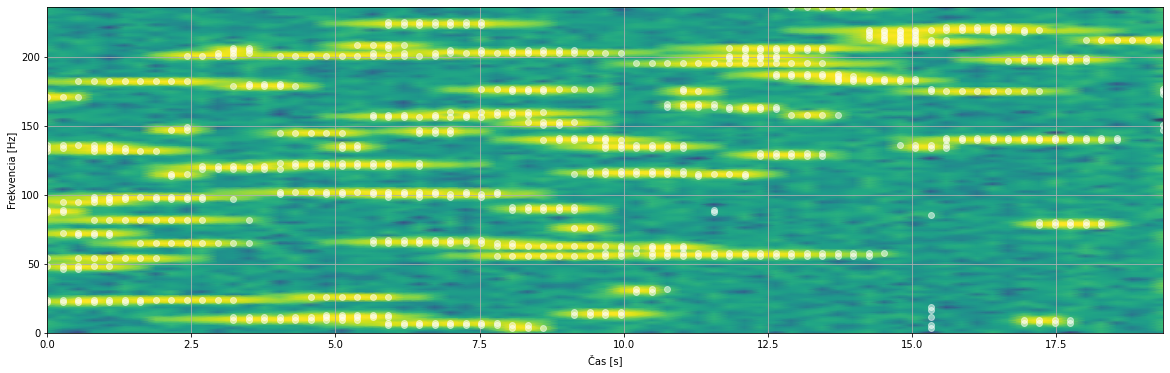
\includegraphics[width=\textwidth]{figures/verification/Sythetic-FFT-A1-476-256.png}
     	\caption{Nájdené špičky algoritmom č.1 v posuvných oknách vyznačené bielym kruhom}
     \end{subfigure}
     \begin{subfigure}{\textwidth}
    	\centering
    	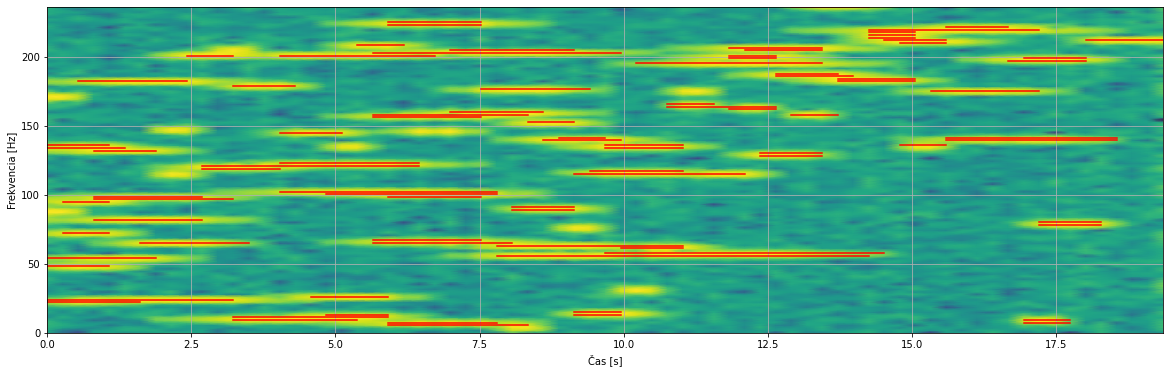
\includegraphics[width=\textwidth]{figures/verification/Sythetic-A1-events.png}
   		\caption{Zachytený priebeh udalostí frekvenčnej zmeny pri $t_{min} = 4$ a $t_{\Delta} = 1$}
     \end{subfigure}
     \caption{Spektrogramy detegovaných špičiek a udalostí pri $f_s = 476$ Hz a $N = 256$}
\end{figure}

Parametre klasifikácie špičiek nájdené mriežkovým hľadaním, s ktorými sme dosiahli na konkrétnom syntetickom signále
najvyššie presnosti sú v tabuľke \ref{tab:grid-serach-parameters}.
\begin{table}[h]
\def\arraystretch{1.1}
\centering
\begin{tabular}{|c|c|ccc|cc|cccc|}
\hline
\multirow{2}{*}{\textbf{\begin{tabular}[c]{@{}c@{}}$f_s$\end{tabular}}} & \multirow{2}{*}{\textbf{\begin{tabular}[c]{@{}c@{}}$n$\end{tabular}}} & \multicolumn{3}{c|}{\textbf{\begin{tabular}[c]{@{}c@{}}Algoritmus 1\end{tabular}}} & \multicolumn{2}{c|}{\textbf{\begin{tabular}[c]{@{}c@{}}Algoritmus 2\end{tabular}}} & \multicolumn{4}{c|}{\textbf{\begin{tabular}[c]{@{}c@{}}Algoritmus 2\end{tabular}}}  \\ \cline{3-11}
                                                                                  &                                                                         & \multicolumn{1}{c|}{\hspace*{3mm}$k$\hspace*{3mm}}         & \multicolumn{1}{c|}{\hspace*{3mm}$\epsilon$\hspace*{3mm}}         & $h_{rel}$       & \multicolumn{1}{c|}{\hspace*{4mm} $k$ \hspace*{4mm}}                               &  $s$                              & \multicolumn{1}{c|}{$t$} & \multicolumn{1}{c|}{$h$} & \multicolumn{1}{c|}{$p$} & $i$ \\ \hline
238                                                                               & 128                                                                     & \multicolumn{1}{c|}{12}          & \multicolumn{1}{c|}{3}                  & 32                & \multicolumn{1}{c|}{2}                                 & 12                                & \multicolumn{1}{c|}{16}  & \multicolumn{1}{c|}{0}   & \multicolumn{1}{c|}{10}  & 8   \\ \hline
238                                                                               & 256                                                                     & \multicolumn{1}{c|}{3}           & \multicolumn{1}{c|}{1}                  & 32                & \multicolumn{1}{c|}{2}                                 & 16                                & \multicolumn{1}{c|}{16}  & \multicolumn{1}{c|}{0}   & \multicolumn{1}{c|}{10}  & 12  \\ \hline
238                                                                               & 512                                                                     & \multicolumn{1}{c|}{3}           & \multicolumn{1}{c|}{4}                  & 32                & \multicolumn{1}{c|}{2}                                 & 26                                & \multicolumn{1}{c|}{10}  & \multicolumn{1}{c|}{4}   & \multicolumn{1}{c|}{38}  & 0   \\ \hline
476                                                                               & 128                                                                     & \multicolumn{1}{c|}{3}           & \multicolumn{1}{c|}{4}                  & 16                & \multicolumn{1}{c|}{2}                                 & 9                                 & \multicolumn{1}{c|}{10}  & \multicolumn{1}{c|}{0}   & \multicolumn{1}{c|}{10}  & 0   \\ \hline
476                                                                               & 256                                                                     & \multicolumn{1}{c|}{12}          & \multicolumn{1}{c|}{4}                  & 32                & \multicolumn{1}{c|}{2}                                 & 12                                & \multicolumn{1}{c|}{16}  & \multicolumn{1}{c|}{0}   & \multicolumn{1}{c|}{10}  & 0   \\ \hline
476                                                                               & 512                                                                     & \multicolumn{1}{c|}{3}           & \multicolumn{1}{c|}{4}                  & 32                & \multicolumn{1}{c|}{1}                                 & 20                                & \multicolumn{1}{c|}{10}  & \multicolumn{1}{c|}{4}   & \multicolumn{1}{c|}{33}  & 0   \\ \hline
952                                                                               & 128                                                                     & \multicolumn{1}{c|}{3}           & \multicolumn{1}{c|}{4}                  & 0                 & \multicolumn{1}{c|}{2}                                 & 5                                 & \multicolumn{1}{c|}{10}  & \multicolumn{1}{c|}{0}   & \multicolumn{1}{c|}{10}  & 0   \\ \hline
952                                                                               & 256                                                                     & \multicolumn{1}{c|}{6}           & \multicolumn{1}{c|}{4}                  & 24                & \multicolumn{1}{c|}{2}                                 & 5                                 & \multicolumn{1}{c|}{16}  & \multicolumn{1}{c|}{0}   & \multicolumn{1}{c|}{10}  & 0   \\ \hline
952                                                                               & 512                                                                     & \multicolumn{1}{c|}{6}           & \multicolumn{1}{c|}{4}                  & 32                & \multicolumn{1}{c|}{2}                                 & 12                                & \multicolumn{1}{c|}{16}  & \multicolumn{1}{c|}{0}   & \multicolumn{1}{c|}{10}  & 0   \\ \hline
\end{tabular}
\caption{Parametre algoritmov detekcie špičiek na syntetických dátach (názvy sú skrátené na prvé písmená)}
\label{tab:grid-serach-parameters}
\end{table}

Manuálnym odladením parametrov na ukážkových záznamoch z vozidiel sme odskúšali rozdiely v schopnostiach algoritmov
na hľadanie špičiek povšimnúť si pretrvávajúce harmonické zložky. Výrez časovo-premenného spektra na obr. \ref{spectrum-slice}
s nájdenými špičkami zvýrazňuje prekážky správneho odlíšenia šumu alebo navzájom splývajúcich kopcov. Niektoré lokálne extrémy
sú prehliadnuté pre nevýraznosť nad svojím okolím alebo pre prílišnú sploštenosť.
\begin{figure}[h]
   \centering
    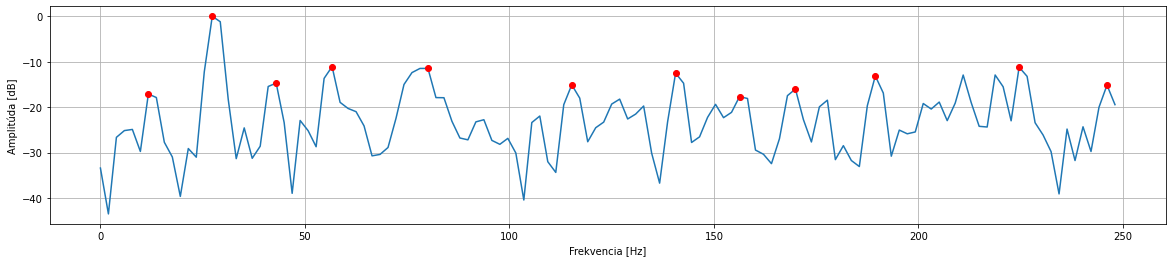
\includegraphics[width=\textwidth]{figures/verification/L83-slice-t-20-A1.png}
   \caption{Prierez spektrogramu okna 256 vzoriek s vrcholmi označenými algoritmom č.1
   v 20. sekunde záznamu \emph{L83\_4940\_Alexyho\_Svantnerova.csv}}
   \label{spectrum-slice}
\end{figure}

Nie je úplne zrejmé aké vodorovné konštelácie výrazných čŕt z obr. \ref{dataset-detection} sú korektne vyznačené,
a ktoré sú primerane agregované do spoločných udalostí. Podstatné frekvencie v stabilnej oblasti medzi časmi 22 a 33
sekundou ako napr. 11, 26, 56 Hz  boli univerzálne zaevidované. Detekcie z iného datasetu sú ilustrované v prílohe.

\begin{figure}[h]
	\centering
     \begin{subfigure}{\textwidth}
        \centering
     	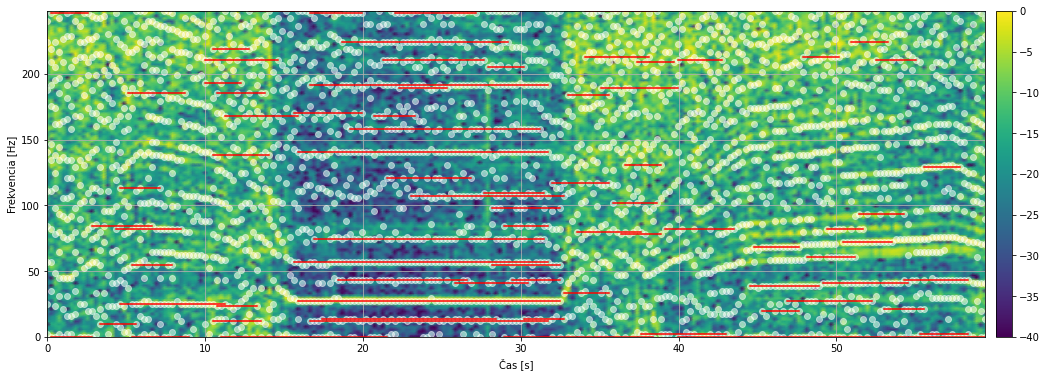
\includegraphics[width=\textwidth]{figures/verification/L83-dataset-A1.png}
     	\caption{Algoritmus č.1: $k = 6$, $\epsilon = 0$, $h_{rel} = 10$}
     \end{subfigure}
     \begin{subfigure}{\textwidth}
    	\centering
        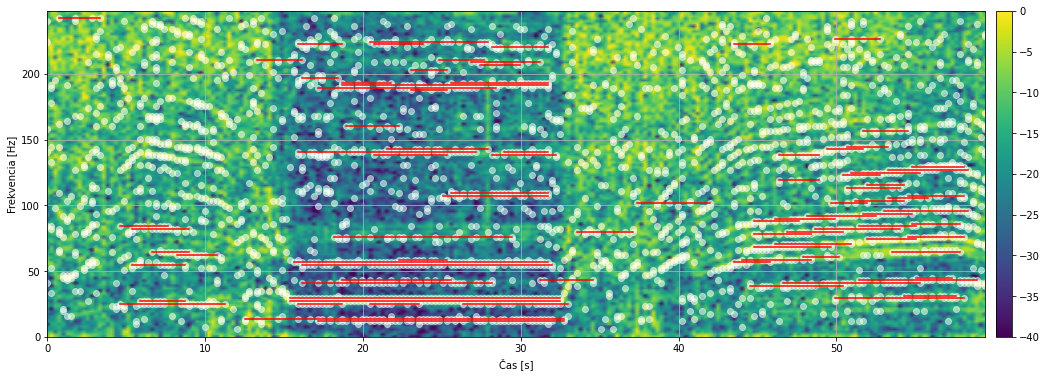
\includegraphics[width=\textwidth]{figures/verification/L83-dataset-A2.png}
        \caption{Algoritmus č.2: $k = 3$, $s = 9$}
     \end{subfigure}
      \begin{subfigure}{\textwidth}
    	\centering
        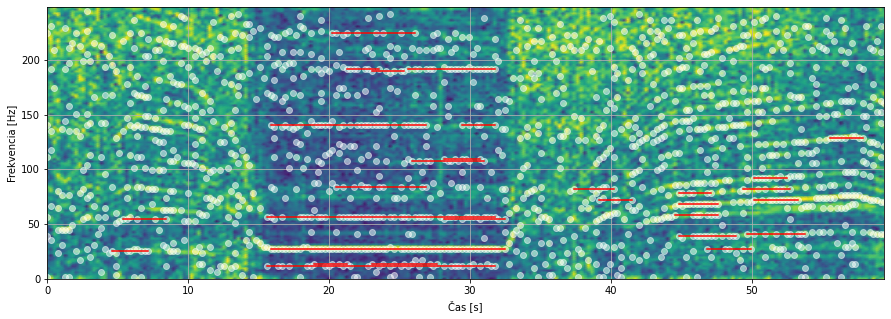
\includegraphics[width=\textwidth]{figures/verification/L83-dataset-A3.png}
        \caption{Algoritmus č.3: $t = 10$, $h = 1$, $p = 10$, $i = 0$}
     \end{subfigure}
     \caption{Detekcia udalostí v datasete \emph{L83\_4940\_Alexyho\_Svantnerova.csv} s $f_s = 500$ Hz, trvaním 60 s, dĺžkou okna 256,
     pri $t_{min} = 10$ a $t_{\Delta} = 4$}
     \label{dataset-detection}
\end{figure}
\cleardoublepage


\chapter{Zhodnotenie} \label{chapter:evaluation}
Zaoberali sme sa meraním vibrácií snímačom trojrozmerného zrýchlenia.
Signálových priebehy sme analyzovali viacerými existujúcimi metódami v časovej a frekvenčnej oblasti.
Podstatou riešeného problému bolo usporiť bezdrôtovo prenášané množstvo informácií, poskytnutím
prehľadu nad sledovanou situáciou upozornením na výskyt a amplitúdu významných frekvencií, či súhrnom
časových úsekov deskriptívnymi štatistikami. Dôležitú etapu v automatizovanej extrakcii
podstatných harmonických zložiek predstavovalo hľadanie špičiek, kde sme porovnali tri odlišné
elementárne koncepcie v literatúre často uplatňované na biologické signály.

Prínos spočíva v navrhnutí postupnosti krokov spracovania dátovej pipeline, špecifikovaním
modifikovateľných parametrov každého stupňa tejto sústavy, a implementácii vzdialene nastaviteľnej
pipeline do firmvéru senzorovej jednotky. Hardvér zariadenia bol poskytnutý už zhotovený.

Na identifikáciu udalostí zmien spektrálneho obsahu vibrácií v čase sme vytvorili nový prúdový algoritmus.
Poradí si s krátkodobými záchvevmi v označenej prítomnosti sekvencie vrcholov minimálnej dĺžky. Účinne pôsobí
v podstate na redukciu šumu z náhlych jednorázových výskytov špičiek. Cez minimálnu testovaciu infraštruktúru
zvolenými sieťovými protokolmi a serializačným formátom sme schopný posielať tematicky kategorizované správy vlastnej
štruktúry. Uznávame, že zotavenie firmvéru z chybových stavov spojené s nedostatkom prostriedkov sa mohlo
hlásiť obšírnejšie ako reštartom alebo zaslaním všeobecnej hlášky.

Validácia detekčných schopností sa opierala o originálny generátor syntetického signálu so šumom podľa
predpisu požadovaných zložiek, ktoré sme na vyjadrenie úspešnosti detekcie pridávali pseudonáhodne.
Stratégie spracovania sa konfrontovali s otrasmi v reálnej premávke datasetmi
zozbieraných s dostupným zariadením.

Program obsadzujúci 65\% voľnej pamäte na inštrukcie je schopný spoľahlivo pracovať s posuvnými
oknami do 512 bodov, v priamočiarejších scenároch kde sú výstupom len udalosti až do 1024 vzoriek.
Posielanie všetkých štatistík sa oplatí nad postupnosť 32 bodov. Počet naraz oznamovaných
zmien frekvencií by za zachovania efektívnosti nemal presiahnuť 12 - 18\% vedierok posuvného
okna. Skutočná priemerná prevalencia 0.5\% a maximálna na úrovni 6\% dokazuje ušetrenie v prenášanom obsahu.
Systém spĺňa kladené obmedzenia na rýchlosť spracovania pri taktovacej frekvencii procesora 160 Hz s ľubovoľnými
nastaveniami. Vyrovnávacia pamäť dokončí obrat cez etapy pipeline pred skompletizovaním ďalšieho posuvného okna.

Vybudovaný model úspešne zakomponovaný na Edge IoT zariadenie tvorí dobrý základ pre početné rozšírenia
vzťahujúce sa hlavne na detailnejšie preskúmanie vplyvov krokov frekvenčnej transformácie a filtrovania,
a možností vyplývajúcich z viaccestnej dátovej pipeline. Mohlo by sa jednať o využitie lepších kompresných vlastností
energetických koeficientov od DCT-IV a MDCT, než FFT. S filtrovaním sa viaže upravenie údaju o tolerancii podľa
aplikovaného kernelu vyhladzovania.

Pokiaľ je predmetom záujmu konkrétny frekvenčný rozsah mohlo by sa autonómne stanoviť ich filtrovanie a najlepšie rozlíšenie.
Rovnako tak sa pre potenciálne produkčné účely ukazuje nepostrádateľnosť samostatnej kalibrácie parametrov hľadania špičiek.
Zaujímavé by bolo prísť s ošetrením cyklického frekvenčného driftu a umožniť označenie profilu známych javov s ich odlíšením pri
notifikáciach. Ďalšia pridaná hodnota by spočívala v určení prevažného priestorového smeru frekvencie alebo koordinácii viacerých senzorov
v spoločnom transportnom boxe.

Dosiaľ dosiahnuté výsledky môžu byť obohatené o silnejšie závery úspešnosti detekcie z opakovaného snímania rôznych stavov
vozidla na vybraných cestách za vypracovania metodiky anotovania skompilovaného datasetu. Za kontrolovanejších podmienok
by sa zariadenie mohlo podrobiť skúšaniu na testovacej lavici.

Softvérové riešenie vychádzajúce z mnohostrannej analýzy problematiky je funkčné a napĺňa intencie
zadania tejto bakalárskej práce.
\cleardoublepage



\pagenumbering{gobble}
%\nocite{*}
\printbibliography[title={Literatúra}]

%Príloha
\addtocontents{toc}{\protect\setcounter{tocdepth}{0}}
\addtocontents{toc}{\cftpagenumbersoff{chapter}}
\appendix
\titleformat{\chapter}{\normalfont\huge\bf}{Príloha \thechapter:}{1em}{}
\renewcommand{\chaptermark}[1]{\markboth{\uppercase{Príloha \thechapter.\ #1}}{}}

\thispagestyle{empty}
\chapter{Plán práce}
\pagenumbering{arabic}
\renewcommand*{\thepage}{A-\arabic{page}}

\section{Zimný semester}

\begin{table}[h!]
\def\arraystretch{1.25}
\begin{tabular}{|l|p{12cm}|}
\hline
\textbf{Obdobie} & \textbf{Náplň práce}                                                                                                                                                                                                                         \\ \hline
1. týždeň         & Základný prehľad relevantnej literatúry.                                                                                                                                                                                                      \\ \hline
2. týždeň         & Štúdium literatúry ohľadom montorovania vibrácií. Pokusný zber dát akcelerácie z MHD pomocou akcelerometra na smartfóne a ich prieskumná analýza.                                             \\ \hline
3. týždeň         & Štúdium článkov o frekvenčnej analýze a rešerš algoritmov na hľadanie špičiek. Implementácia objavených prístupov hľadania špičiek a aplikovanie na merania vibrácií z električiek a autobusu. \\ \hline
4. týždeň         & Flashovanie firmvéru na vývojový kit iCOMOX od Shiratech.                                                                                                                                                                                                  \\ \hline
5. týždeň         & Osnova práce s referenciami na nájdenú literatúru.                                                                                                                                                                                            \\ \hline
6. týždeň         & Firmvér pre dosku na platforme ESP32 pre záznam akceleračných dát na SD kartu cez OpenLog \\ \hline
7. týždeň         & Merania vibrácií v MHD a analýza získaných záznamov v Jupyter notebooku. Doplnenie zdrojov pre časti osnovy s málo referenciami.                                                                  \\ \hline
8. týždeň         & Sekcia 2.1. práce o monitorovaní vibrácií a šoku.                                                                                                                                                                                             \\ \hline
9. týždeň         & Doplnenie typov akcelerometrov a časti o numerickej kvadratúre k sekcii 2.1. Úvod do sekcie 2.2. o analýze v časovej doméne.                                                                       \\ \hline
10. týždeň        & Deskriptívne štatistiky a algoritmy na identifikáciu špičiek.                                                                                                                                                                                 \\ \hline
11. týždeň        & Sekcia 2.2. o frekvenčnej a časovo-frekvenčnej analýze signálu.                                                                                                                                                                               \\ \hline
12. týždeň        & Sekcia 2.3 o architektúre senzorových sietí a ich obmedzeniach. Návrh riešenia a úvod k priebežnej správe BP1. \\ \hline
13. týždeň        & Zapracované pripomienky k prezentovanému návrhu.                                                                                                                                                                             \\ \hline
\end{tabular}
\end{table}

Rozvrhnutie pred začiatkom zimného semestra sa držalo dvoch oporných termínov a síce 6. týždňa a 12. týždňa.
V 6. týždni sme chceli zavŕšiť rešerš podstatných zdrojov literatúry podľa predstavy o charaktere vibračných signálov
nadobutnutých aj prieskumnými meraniami. V druhej polovici semestra sme tak vedeli zostaviť osnovu a každý týždeň
sa venovať jednej sekcii analýzy až do 12. týždňa.

\clearpage
\newpage


\section{Letný semester}
\begin{table}[h!]
\def\arraystretch{1.25}
\begin{tabular}{|l|p{12cm}|}
\hline
\textbf{Obdobie} & \textbf{Náplň práce}                                                                                                                                            \\ \hline
1. týždeň        & Tvorba generátora syntetického signálu s mechanizmom vyhodnocovania metrík  klasifikácie detektorov.                                                            \\ \hline
2. týždeň        & Pripravenie vývojového prostredia s ESP-IDF SDK a výber  vhodných knižníc  pre DSP a Message Pack.                                                              \\ \hline
3. týždeň        & Odlaďovanie ovládania hardvérových periférií: akcelerometer, pripojenie na WiFi.  Návrh krokov spracovania údajov.                                                \\ \hline
4. týždeň        & Zakomponovanie posielania vzoriek cez MQTT. Validácia na syntetických dátach rozdelených na trénovaciu a testovaciu sadu.                                       \\ \hline
5. týždeň        & Implementácia kostry spracovania na IoT zariadenie. Message Pack serializácia  konfigurácie a jej publikovanie  cez MQTT. \\ \hline
6. týždeň        & Parser prijatej konfigurácie, uloženie a aplikácia nastavení na zariadení.  Optimalizácia alokovania dostupnej pamäte.                                          \\ \hline
7. týždeň        & Návrh algoritmu na identifikáciu udalostí. Jednoduché jednotkové testy na validáciu funkčnosti systému a prvotné výkonnostné testy. Tvorba doxygen dokumentácie. \\ \hline
8. týždeň        & Experimentálne merania pamäťovej a časovej efektivity. Vyhodnocovanie úspešnosti hľadania špičiek podľa hyperparametrov. \\ \hline
9. týždeň        & Ilustrácie a diagramy zahrnuté do kapitoly návrhu. \\ \hline
10. týždeň       & Písanie textu 3. kapitoly ,,Návrh riešenia'' a 4. kapitoly ,,Implementácia''. \\ \hline
11. týždeň       & Písanie textu, vyhotovenie grafov a tabuliek pre zvyšné kapitoly  hlavnej časti práce. \\ \hline
12. týždeň       & Doplnenie príloh práce, najmä technickej dokumentácie a  používateľskej príručky.                                                                                 \\ \hline
13. týždeň       & Prezentácia celkového vypracovania vedúcemu práce a zapracovanie pripomienok.                                                                                                           \\ \hline
\end{tabular}
\end{table}

Pôvodný plán vychádzal z trojtýždenných cyklov, kde po každom by kompletná daná časť systému, v skutočnosti sa
prirodzene prelínali a dopĺňali. Do konca 3. týždňa sme plánovali odladenie modelov na monitorovanie vibrácií na základe
analyzovaných algoritmov a meranie úspešnosti na synteticky generovaných dátach. Do 6.týždňa mala byť funkčný
záznamom udalostí na pamäťovú kartu vo firmvéri. Do 9. týždňa sa mala uskutočniť optimalizácia posielaných dát
a vzdialená konfigurácia. Na posledný beh pripadali experimenty a ich vyhodnotenie, počas ktorých bol už písaný text práce.
Konzultácie raz za dva týždne tvorili kontrolné body, kedy sme konfrontovali plnenie plánu s postupom.
\clearpage


\thispagestyle{empty}
\chapter{Technická dokumentácia}
\pagenumbering{arabic}
\renewcommand*{\thepage}{B-\arabic{page}}

\section{Doxygen dokumentácia}
Nástroj Doxygen zhotovil podľa komentárov v zdrojom kóde prehľadnú technickú dokumentáciu,
ktorá je po typografickej úprave súčasťou tejto prílohy.

\subsection{Moduly}
\begin{itemize}[noitemsep, topsep=0pt]
	\item \textbf{Udalosti} (\ref{modules:events}) - Binárne klasifikátory na označenie význačných úrovní v posuvnom okne vzoriek. 
	Zdrojový kód: \verb|events.h|, \verb|events.c|.
	\item \textbf{Akcelerometer} (\ref{modules:imu}) - Adaptér pre SPI rozhranie senzora LSM9DS1 lineárnej 3D akcelerácie (IMU).
	Zdrojový kód: \verb|inertial_unit.h|, \verb|inertial_unit.c|
	\item \textbf{Hardvérové adaptéry} (\ref{modules:hardware}) - Rozhrania na komunikáciu s perifériami.
	Zdrojový kód: \verb|peripheral.h|, \verb|peripheral.c|
	\item \textbf{Dátová pipeline} (\ref{modules:pipeline}) - Fázy spracovania zdrojového signálu. Zdrojový kód: \verb|pipeline.h|
	\begin{itemize}[noitemsep, topsep=0pt]
		\item \textbf{Oknové funkcie} - \verb|window.c|
		\item \textbf{Správa pamäti pipeline} - \verb|pipeline.c|
		\item \textbf{Fázy spracovania oknovaného signálu} - \verb|pipeline.c|
		\item \textbf{Message Pack serializácia} - Serializácia a parsovanie nameraných dát a konfigurácie. \verb|serialize.c|
	\end{itemize}
	\item \textbf{Deskriptívna štatistika} (\ref{modules:statistics}) - výpočet popisných štatistík. Zdrojový kód: \verb|statistics.h|, \verb|statistics.c|
\end{itemize}


\subsection{Udalosti} \label{modules:events}
Modul s binárnymi klasifikátormi na označenie význačných úrovní v posuvnom okne vzoriek.

\subsubsection*{Dátové štruktúry}
\textbf{struct SpectrumEvent} - Stav udalosti frekvenčného vedierka.
\begin{itemize}[noitemsep, topsep=0pt]
	\item \verb|SpectrumEventAction action|: Značka vymedzenia udalosti
	\item \verb|uint32_t start|: Časová pečiatka alebo poradie posuvného okna, kedy začala aktuálne aktívna udalosť
	\item \verb|uint32_t duration|: Trvanie aktívnej udalosti v počte posuvných okien
	\item \verb|int32_t last_seen|: Počet posuvných okien do minulosti, kedy bol detegovaný posledný výskyt špičky vo frekvencii
	\item \verb|float amplitude|: Priemerná amplitúda frekvenčného vedierka počas trvania udalosti
\end{itemize}

\subsubsection*{Enumerácie}
\textbf{enum SpectrumEventAction} - Časové vymedzenie udalosti frekvenčného spektra.
	\begin{itemize}[noitemsep, topsep=0pt]
		\item \verb|SPECTRUM_EVENT_NONE|: Udalosť prebieha alebo žiadna nie je aktívna
		\item \verb|SPECTRUM_EVENT_START|: Značka začiatku udalosti
		\item \verb|SPECTRUM_EVENT_FINISH|: Značka ukončenia udalosti
	\end{itemize}

\subsubsection*{Funkcie}
\begin{lstlisting}[style=docs]
void find_peaks_above_threshold (
    bool *peaks, const float *y, int n, float t
) 
\end{lstlisting}
    Hľadanie špičiek absolútnou prahovou úrovňou amplitúdy signálu. \\
\textbf{Parametre}:
\begin{itemize}[noitemsep, topsep=0pt]
	\item \textbf{peaks} (out): Nájdené špičky v signále. Dĺžka poľa musí byť rovnaká počtu vzoriek
	\item \textbf{y} (in): Vzorky signálu 
	\item \textbf{n} (in): Počet vzoriek 
	\item \textbf{t} (in) Prahová úroveň amplitúdy. Odporúčaná hodnota je z prípustných hodnôt rozsahu pre vzorky 
\end{itemize}
\bigbreak
\hrule

\begin{lstlisting}[style=docs]
void find_peaks_neighbours (
    bool *peaks, const float *y, int n,  int k, 
    float e, float h_rel, float h
)
\end{lstlisting}
   Hľadanie špičiek s algoritmom význačnosti vrchola spomedzi susedov. \\ $ f[t-i] < f[t] > f[t+i],\quad \forall i \in 1, 2, ..., k $ \\
\textbf{Parametre}:
\begin{itemize}[noitemsep, topsep=0pt]
	\item \textbf{peaks} (out): Nájdené špičky v signále. Dĺžka poľa musí byť rovnaká počtu vzoriek
	\item \textbf{y} (in): Vzorky signálu 
	\item \textbf{n} (in): Počet vzoriek 
	\item \textbf{k} (in): Počet najbližších uvažovaných susedov na každú zo strán od kandidátnej špičky $[t-k; t+k]$;  Rozsah: $[1, n / 2]$
	\item \textbf{e} (in): Relatívna tolerancia pre vyššiu úroveň v susedstve od vrchola
	\item \textbf{h\_rel} (in): Minimálna relatívna výška špičky v susedstve
 	\item \textbf{h} (in): Absolútna prahová úroveň amplitúdy špičky
\end{itemize}
\bigbreak
\hrule

\begin{lstlisting}[style=docs]
void find_peaks_zero_crossing (
	bool *peaks, const float *y, int n, int k, float slope
)
\end{lstlisting}
   Hľadanie špičiek s algoritmom prechodu nulou do záporu. $\Delta f[i] = 0$ \\
\textbf{Parametre}:
\begin{itemize}[noitemsep, topsep=0pt]
	\item \textbf{peaks} (out): Nájdené špičky v signále. Dĺžka poľa musí byť rovnaká počtu vzoriek
	\item \textbf{y} (in): Vzorky signálu 
	\item \textbf{n} (in): Počet vzoriek 
	\item \textbf{k} (in): Dĺžka sečnice na každú stranu od kandidátnej špičky $[t-k; t+k]$; Rozsah: $[1, n / 2]$
	\item \textbf{slope} (in): Prahová úroveň strmosti kopca, čiže rozdielu medzi hladiny medzi koncami sečnice. Rozsah: $slope \geq 0 $
\end{itemize}
\bigbreak
\hrule
\newpage
\begin{lstlisting}[style=docs]
void find_peaks_hill_walker (
	bool *peaks, const float *y, int n, 
	float tolerance, int hole, 
	float prominence, float isolation
)
\end{lstlisting}
   Hľadanie špičiek s modikovaným algoritmom horského turistu. \\
\textbf{Parametre}:
\begin{itemize}[noitemsep, topsep=0pt]
	\item \textbf{peaks} (out): Nájdené špičky v signále. Dĺžka poľa musí byť rovnaká počtu vzoriek
	\item \textbf{y} (in): Vzorky signálu 
	\item \textbf{n} (in): Počet vzoriek 
	\item \textbf{tolerance} (in): Prahová úroveň vo vertikálnej osi. Rozsah: $[\min(y), \max(y)]$
 	\item \textbf{hole} (in): Prahová úroveň v horizontálnej osi. Rozsah: $[0, n]$
 	\item \textbf{prominence} (in):  Relatívna výška oproti predošlej navštívenej doline. Rozsah: $[0, \max(y) - \min(y)]$
 	\item \textbf{isolation} (in)  Vzdialenosť ku najbližšiemu predošlému vrcholu. Rozsah: $[0, n]$
\end{itemize}
\bigbreak
\hrule

\begin{lstlisting}[style=docs]
void event_init (SpectrumEvent *events, uint16_t bins)
\end{lstlisting}
   Nastavenie počiatočného stavu online detektora udalostí vo frekvenciách. \\
\textbf{Parametre}:
\begin{itemize}[noitemsep, topsep=0pt]
	\item \textbf{events} (out): Pole udalostí frekvenčného spektra
	\item \textbf{bins} (in): Počet frekvenčných vedierok a zároveň dĺžka poľa udalostí
\end{itemize}
\bigbreak
\hrule

\begin{lstlisting}[style=docs]
size_t event_detection (
	size_t t, SpectrumEvent *events, const bool *peaks, 
	const float *spectrum, uint16_t bins,
	uint16_t min_duration, uint16_t time_proximity
)
\end{lstlisting}
   Online detekcia zmien v časovom priebehu frekvenčných spektier. \\
\textbf{Parametre}:
\begin{itemize}[noitemsep, topsep=0pt]
\item \textbf{t}: Poradové číslo posuvného okna. S každým ďalším volaním funkcie musí byť navýšené o 1 
\item \textbf{events}: Pole udalostí frekvenčného spektra s dĺžkou počtu vedierok
\item \textbf{peaks} (in): Nájdené špičky vo aktuálnom frekvenčnom spektre jedným z klasifikátorov \emph{find\_peak\_*}
\item \textbf{spectrum} (in): Frekvenčné spektrum aktuálneho posuvného okna vzoriek na zistenie priemernej amplitúdy udalostí
\item \textbf{bins} (in): Počet frekvenčných vedierok
\item \textbf{min\_duration} (in): Minimálne trvanie po koľkých oknách je vyhlásená špička za udalosť. Udáva oneskorenie vyhlásenia začiatku udalosti.
\item \textbf{time\_proximity} (in): Najväčšia vzdialenosť súvislej udalosti v počte okien. Najväčšia dĺžka časovej medzery medzi nájdenými špičkami. Udáva oneskorenie vyhlásenia ukončenia udalosti.
 
\item \textbf{Návratová hodnota}: Počet detegovaných zmien, čiže začiatočných a koncov udalostí v danom spektre posuvného okna
\end{itemize}
\bigbreak
\hrule


\subsection{Akcelerometer} \label{modules:imu}
Modul adaptéra pre SPI rozhranie senzora LSM9DS1 lineárnej 3D akcelerácie (IMU)

\subsubsection*{Dátové štruktúry}
\textbf{struct InertialUnit} - Inerciálna meracia jednotka.
\begin{itemize}[noitemsep, topsep=0pt]
	\item \verb|gpio_num_t clk|: GPIO pin SPI hodinového signálu
	\item \verb|gpio_num_t miso|: GPIO pin SPI Master In Slave Out
	\item \verb|gpio_num_t xgcs|: GPIO pin SPI Chip select akcelometra a gyroskopu
	\item \verb|gpio_num_t mcs|: GPIO pin SPI Chip select magnetometra
	\item \verb|gpio_num_t int1|: GPIO vstup prerušenia č.1
	\item \verb|gpio_num_t int2|: GPIO vstup prerušenia č.2
	\item \verb|gpio_num_t en_data|: GPIO vstup príznaku pripravených dát
	\item \verb|gpio_num_t isr_int1|: Podprogram prerušenia pre INT č.1
	\item \verb|gpio_num_t isr_int2|: Podprogram prerušenia pre INT č.2
	\item \verb|spi_host_device_t spi|: SPI zbernica
	\item \verb|spi_device_handle_t dev|: SPI zariadenie pre akcelerometer
	\item \verb|AccelerationPrecision precision|: Citlivosť akcelerometra v mg/LSB
\end{itemize}

\subsubsection*{Enumerácie}
\textbf{enum AccelerationRange} - Dynamický rozsah akcelerometra v g.
	\begin{itemize}[noitemsep, topsep=0pt]
		\item \verb|IMU_2G|: Rozsah $\pm 2\;\mathrm{g}  = \pm 19.6133 \;\mathrm{m/s^2}$
		\item \verb|IMU_4G|: Rozsah $ \pm 4\;\mathrm{g} = \pm 39.2266 \;\mathrm{m/s^2}$
		\item \verb|IMU_8G|: Rozsah $ \pm 8\;\mathrm{g}  = \pm 78.4532 \;\mathrm{m/s^2}$
		\item \verb|IMU_16G|: Rozsah $ \pm 16\;\mathrm{g}  = \pm 156.9064 \;\mathrm{m/s^2}$
		\item \verb|IMU_RANGE_COUNT|: Počet možností nastavenia rozsahu na účely serializácie
	\end{itemize}
\bigbreak
\noindent\textbf{typedef float AccelerationPrecision} - Citlivosť akcelerometra podľa dynamického rozsahu v mg/LSB.

\subsubsection*{Funkcie}
\begin{lstlisting}[style=docs]
esp_err_t imu_setup(InertialUnit *imu)
\end{lstlisting}
   Inicializácia senzora lineárnej akcelerácie. \\
\textbf{Parametre}:
\begin{itemize}[noitemsep, topsep=0pt]
	\item \textbf{imu}: Senzor
	\item \textbf{Návratová hodnota}: Úspešnosť inicializácie senzora
\end{itemize}
\bigbreak
\hrule

\begin{lstlisting}[style=docs]
void imu_acceleration_range (
	InertialUnit *imu, AccelerationRange range
)
\end{lstlisting}
   Nastavenie dynamického rozsah lineárneho 3D akcelerometra v $g$. \\
\textbf{Parametre}:
\begin{itemize}[noitemsep, topsep=0pt]
	\item \textbf{imu}: Senzor
	\item \textbf{range}: Dynamický rozsah akcelerometra
\end{itemize}
\bigbreak
\hrule

\begin{lstlisting}[style=docs]
void imu_output_data_rate (InertialUnit *imu, uint16_t fs)
\end{lstlisting}
   Nastavenie výstupného dátového toku (ODR) akcelerometra podľa vzorkovanej frekvencie. \\
\textbf{Parametre}:
\begin{itemize}[noitemsep, topsep=0pt]
	\item \textbf{imu}: Senzor
	\item \textbf{fs}: Vzorkovacia frekvencia v Hz. Hardvér povoľuje max. ODR 956 Hz
\end{itemize}
\bigbreak
\hrule

\begin{lstlisting}[style=docs]
void imu_acceleration (
	InertialUnit *imu, float *x, float *y, float *z
)
\end{lstlisting}
   Meranie aktuálnej hodnoty 3D akcelerácie v $m/s^2$. \\
\textbf{Parametre}:
\begin{itemize}[noitemsep, topsep=0pt]
	\item \textbf{imu}: Senzor
	\item \textbf{x} (out): Zrýchlenie v osi x. Rozsah je podľa nastavenia dynamického rozsahu.
 	\item \textbf{y} (out): Zrýchlenie v osi y
    \item \textbf{z} (out): Zrýchlenie v osi z
\end{itemize}


\subsection{Hardvérové adaptéry} \label{modules:hardware}

\subsubsection*{Dátové štruktúry}
\textbf{struct OpenLog} - SparkFun OpenLog - zaznenávač údajov na SD kartu cez sériovú linku.
\begin{itemize}[noitemsep, topsep=0pt]
	\item \verb|gpio_num_t vcc|: GPIO pin na ovládanie napájania cez FET tranzistor
	\item \verb|uint8_t uart|: Číslo UART rozhrania
	\item \verb|gpio_num_t rx|: GPIO pin UART RX
	\item \verb|gpio_num_t tx|: GPIO pin UART TX
	\item \verb|int baudrate|: Symbolová rýchlosť komunikácie. Rovnaká rýchlosť musí byť nastavená v \verb|config.txt| na SD karte
	\item \verb|int buffer|: Dĺžka vyrovnávacej pamäte pre UART
\end{itemize}
\bigbreak

\noindent\textbf{struct MqttAxisTopics} - MQTT témy pre os zrýchlenia.
\begin{itemize}[noitemsep, topsep=0pt]
	\item \verb|char stats[TOPIC_LENGTH]|: Názov témy pre štatistické údaje
	\item \verb|char spectra[TOPIC_LENGTH]|: Názov témy pre frekvenčné spektrum
	\item \verb|char events[TOPIC_LENGTH]|: Názov témy pre udalosti zmeny spektra
\end{itemize}


\subsubsection*{Funkcie}
\begin{lstlisting}[style=docs]
void axis_mqtt_topics (MqttAxisTopics *topics, int axis)
\end{lstlisting}
   Poskladanie názvu MQTT tém pre odosieanie dát o osi akcelerácie. \\
\textbf{Parametre}:
\begin{itemize}[noitemsep, topsep=0pt]
	\item \textbf{topics} (out): MQTT témy zložené s označením osi x, y, z
	\item \textbf{axis} (in): Index osi vektora akcelerácie: 0, 1, 2 
\end{itemize}
\bigbreak
\hrule

\begin{lstlisting}[style=docs]
void clock_reconfigure (uint16_t frequency)
\end{lstlisting}
   Zmena frekvencie časovača. \\
\textbf{Parametre}:
\begin{itemize}[noitemsep, topsep=0pt]
	\item \textbf{frequency} (in):	Vzorkovacia frekvencia v Hz 
\end{itemize}
\bigbreak
\hrule

\begin{lstlisting}[style=docs]
void clock_setup (uint16_t frequency, timer_isr_t action)
\end{lstlisting}
   Spustenie časovača na vzorkovanie signálu. \\
\textbf{Parametre}:
\begin{itemize}[noitemsep, topsep=0pt]
	\item \textbf{frequency} (in): Vzorkovacia frekvencia v Hz
	\item \textbf{action} (in):	Obsluha prerušenia časovača s predpisom: \\ \verb|bool IRAM_ATTR f(void *args)|
\end{itemize}
\bigbreak
\hrule

\begin{lstlisting}[style=docs]
void mqtt_event_handler (
	void *handler_args, esp_event_base_t base, 
	int32_t event_id, void *event_data
)
\end{lstlisting}
Predbežná deklarácia spätného volania. Implementáciu musí poskytnúť hlavný program. Používa sa v \verb|mqtt_setup()|. \\
\bigbreak
\hrule

\begin{lstlisting}[style=docs]
esp_mqtt_client_handle_t mqtt_setup (
	const char *broker_url
)
\end{lstlisting}
   Pripojenie sa k MQTT broker a zaregistrovanie spätného volanie pre všetky udalosti. \\
\textbf{Parametre}:
\begin{itemize}[noitemsep, topsep=0pt]
	\item \textbf{broker\_url}: URL MQTT broker 
\end{itemize}
\bigbreak
\hrule

\begin{lstlisting}[style=docs]
esp_err_t nvs_load (
	Configuration *conf, Provisioning *login
)
\end{lstlisting}
   Načítanie nastavení systému z nevolatilného úložiska. \\
\textbf{Parametre}:
\begin{itemize}[noitemsep, topsep=0pt]
	\item \textbf{conf} (out): Globálne nastavenia spracovania dát
	\item \textbf{login} (out): Nastavenie sieťového pripojenia
\end{itemize}
\bigbreak
\hrule

\begin{lstlisting}[style=docs]
esp_err_t nvs_save_config (const Configuration *conf)
\end{lstlisting}
   Uloženie nastavení systému na nevolatilné úložisko. \\ Používa sa v \verb|mqtt_event_handler()|. \\
\textbf{Parametre}:
\begin{itemize}[noitemsep, topsep=0pt]
	\item \textbf{conf} (in): Globálne nastavenia spracovania dát
\end{itemize}
\bigbreak
\hrule

\begin{lstlisting}[style=docs]
esp_err_t nvs_save_login (const Provisioning *login)
\end{lstlisting}
   Uloženie nastavení sieťového pripojenia na nevolatilné úložisko. \\ Používa sa v \verb|mqtt_event_handler()|. \\
\textbf{Parametre}:
\begin{itemize}[noitemsep, topsep=0pt]
	\item \textbf{login} (in): Nastavenie sieťového pripojenia 
\end{itemize}
\bigbreak
\hrule

\begin{lstlisting}[style=docs]
void openlog_setup (OpenLog *logger)
\end{lstlisting}
Nastavenie UART rozhrania pre zariadenie OpenLog.
\bigbreak
\hrule

\begin{lstlisting}[style=docs]
void wifi_connect (wifi_config_t *wifi_config)
\end{lstlisting}
Pripojenie sa k Wifi AP blokujúce.


\subsection{Dátová pipeline} \label{modules:pipeline}

\subsubsection*{Dátové štruktúry}
\noindent\textbf{struct SamplingConfig} - Nastavenie vzorkovania signálu.
\begin{itemize}[noitemsep, topsep=0pt]
	\item \verb|uint16_t frequency|: Vzorkovacia frekvencia v Hz. Najviac \verb|MAX_FREQUENCY|
	\item \verb|AccelerationRange range|: Dynamický rozsah akcelerometra
	\item \verb|uint16_t n|: Veľkosť posuvného okna. Musí byť mocninou dvojky a najviac \verb|MAX_BUFFER_SAMPLES|
	\item \verb|float overlap|: Pomer prekryvu posuvných okien. Rozsah: 0 až \verb|MAX_OVERLAP|
	\item \verb|bool axis[AXIS_COUNT]|: Osi akcelerácie povolené na spracovanie
\end{itemize}
\bigbreak

\noindent\textbf{struct SmoothingConfig} - Nastavenie vyhladzovania časovo premenného signálu alebo frekvenčného spektra.
\begin{itemize}[noitemsep, topsep=0pt]
	\item \verb|bool enable|: Vyhladzovanie signálu povolené
	\item \verb|uint16_t n|: Dĺžka konvolučnej masky
	\item \verb|uint8_t repeat|: Počet prechodov konvolučnej masky.\\ Najviac \verb|MAX_SMOOTH_REPEAT|
\end{itemize}
\bigbreak

\noindent\textbf{struct StatisticsConfig} - Nastavenie zberu štatistík posuvného okna.
\begin{itemize}[noitemsep, topsep=0pt]
	\item \verb|bool min|: Výpočet minimálnej hodnoty povolený
	\item \verb|bool max|: Výpočet maximálnej hodnoty povolený
	\item \verb|bool rms|: Výpočet strednej kvadratickej odchýlky povolený
	\item \verb|bool mean|: Výpočet aritmetického priemeru povolený
	\item \verb|bool variance|: Výpočet rozptylu povolený
	\item \verb|bool std|: Výpočet smerodajnej odchýlky povolený
	\item \verb|bool skewness|: Výpočet šikmosti povolený
	\item \verb|bool kurtosis|: Výpočet špicatosti povolený
	\item \verb|bool median|: Výpočet mediánu povolený
	\item \verb|bool mad|: Výpočet mediánovej absolútnej odchýlky povolený
	\item \verb|bool correlation|: Výpočet korelácie medzi osami povolený
\end{itemize}
\bigbreak

\noindent\textbf{struct FFTTransformConfig} - Nastavenie frekvenčnej transformácie.
\begin{itemize}[noitemsep, topsep=0pt]
	\item \verb|WindowTypeConfig window|: Oknová funkcia
	\item \verb|FrequencyTransform func|: Typ frekvenčnej transformácie
	\item \verb|bool log|: Prevod magnitúdy frekvencie do dB
\end{itemize}
\bigbreak

\noindent\textbf{struct SaveFormatConfig} - Nastavenia ukladania a posielania spracovaných dát.
\begin{itemize}[noitemsep, topsep=0pt]
	\item \verb|bool local|: Záznam vzoriek na SD kartu povolený. OpenLog bude zapnutý po spustení
	\item \verb|bool mqtt|: Posielanie cez MQTT povolené. Wifi a MQTT klient bude zapnutý po spustení. Pozor: po deaktivácii
	sa zariadenie nedá vzdialene rekonfigurovať. Na znovu povolenie sa musí nahrať firmvér so touto možnosťou povolenou. 
	\item \verb|bool mqtt_stats|: Odosielanie štatistík cez MQTT na topic \\ podľa \verb|MQTT_TOPIC_STATS|
	\item \verb|bool mqtt_events|:  Odosielanie zmien spektra cez MQTT na topic \\ podľa \verb|MQTT_TOPIC_EVENT|
	\item \verb|SendUnprocessed mqtt_samples|:  Odosielanie nespracovaných vzoriek alebo frekvencií cez MQTT na topic \\ podľa \verb|MQTT_TOPIC_STREAM|, \verb|MQTT_TOPIC_SPECTRUM|.
	\item \verb|uint16_t subsampling|: Podvzorkovanie pre záznam vzoriek bez ďalšieho spracovania. Preskočí sa každých \verb|subsampling| vzoriek
\end{itemize}
\bigbreak

\noindent\textbf{struct FFTTransformConfig} - Nastavenia algoritmov na detekciu udalostí a ich parametrov (popis sa nachádza pri 
funkciách z modulu ,,Udalosti'' \ref{modules:events}).
\bigbreak

\noindent\textbf{struct Configuration} - Systémová konfigurácia pipeline spracovania vzoriek z akcelerometra.
\bigbreak

\noindent\textbf{struct Provisioning} - Sieťové nastavenia pre pripojenie na Wifi AP s WPA2 a MQTT broker.
\bigbreak

\noindent\textbf{struct Correlation} - Medzivýsledky korelácie zdieľanej všetkými osami spracovania s prístupom
cez zahrnutú synchronizačnú bariéru.
\bigbreak

\noindent\textbf{struct Statistics} - Výsledky všetkých dostupných štatistík.
\bigbreak

\noindent\textbf{struct BufferPipelineKernel} - Vyrovnávacie pamäte spoločné pre celú pipeline.
\bigbreak

\noindent\textbf{struct BufferPipelineAxis} - Vyrovnávacie pamäte samostatné pre každú os akcelerácie.
\bigbreak

\noindent\textbf{struct Sender} - Fronta pre záznam vzoriek bez ďalšiho spracovania.
\bigbreak

\subsubsection*{Konštanty}
V zátvorkách sú uvedené predvolené hodnoty
\begin{itemize}[noitemsep, topsep=0pt]
	\item \verb|AXIS_COUNT|: Celkový počet osí akcelerácie (3)
	\item \verb|MAX_MPACK_FIELDS_COUNT|: Maximálny počet dvojíc ,,kľúč - hodnota'' v Message Pack slovníku (20)
	\item \verb|SAMPLES_QUEUE_SLOTS|: Násobok veľkosti posuvného okna ako počet vzoriek čakajúcich na spracovanie vo fronte (3)
	\item \verb|MAX_CREDENTIALS_LENGTH|: Maximálna dĺžka prihlasovacieho údaju Wifi pripojenia (64)
	\item \verb|MAX_MQTT_URL|: Dĺžka URL adresy na MQTT broker (256)
	\item \verb|MAX_BUFFER_SAMPLES|: Najdlhšie povolené posuvné okno, vyššia mocnina 2 ako 1024 sa nezmestí do DRAM (1024)
	\item \verb|MAX_FREQUENCY|: Najvyššia vzorkovacia frekvencia daná fyzickým obmedzením akcelerometra (952)
	\item \verb|MAX_OVERLAP|:  Maximálny prekryv posuvných okien (0.8)
	\item \verb|MAX_SMOOTH_REPEAT|:  Maximálny počet prechodu konvolučnej masky vyhladzovacieho filtra (8)
	\item \verb|LARGEST_MESSAGE|: Najväčšia veľkosť vyrovnávacej pamäte pre serializáciu vzoriek (14000)
	\item \verb|LARGEST_CONFIG|: Najväčšia veľkosť serializovanej konfigurácie (480)
\end{itemize}


\subsubsection*{Enumerácie}
\noindent\textbf{enum WindowTypeConfig} - Oknové funkcie.
	\begin{itemize}[noitemsep, topsep=0pt]
		\item \verb|BOXCAR_WINDOW|: Obdĺžníkové okno
		\item \verb|BARTLETT_WINDOW|: Bartlettovo okno
		\item \verb|HANN_WINDOW|: Hannovo okno
		\item \verb|HAMMING_WINDOW|: Hammingovo okno
		\item \verb|BLACKMAN_WINDOW|: Blackmanovo okno
		\item \verb|WINDOW_TYPE_COUNT|: Počet dostupných oknových funkcií. Potrebné pre serializáciu.
	\end{itemize}
\bigbreak

\noindent\textbf{enum PeakFindingStrategy} - Algoritmy na hľadanie špičiek.
	\begin{itemize}[noitemsep, topsep=0pt]
		\item \verb|THRESHOLD|: Špičky nad prahovou úrovňou.
		\item \verb|NEIGHBOURS|: Špičky najvýznačnejšieho bodu spomedzi susedov.
		\item \verb|ZERO_CROSSING|: Špičky prechodou nulou do záporu.
		\item \verb|HILL_WALKER|: Špičky algoritmom horského turistu. 
		\item \verb|STRATEGY_COUNT|: Počet možností na účely serializácie
	\end{itemize}
\bigbreak

\noindent\textbf{enum FrequencyTransform} - Frekvenčné transformácie.
	\begin{itemize}[noitemsep, topsep=0pt]
		\item \verb|DFT|: Rýchla Fourierová transformácia radix-2
		\item \verb|DCT|: Konsínusová transformácia DCT-II
		\item \verb|TRANSFORM_COUNT|: Počet dostupných frekvenčných transformácií. Potrebné pre serializáciu
	\end{itemize}
\bigbreak

\noindent\textbf{enum SendUnprocessed} - Doména odosielaných nespracovaných vzoriek.
	\begin{itemize}[noitemsep, topsep=0pt]
		\item \verb|RAW_NONE_SEND|: Žiadne nespracované vzorky 	
		\item \verb|RAW_TIME_SEND|: Nespracované vzorky v časovej oblasti 	
		\item \verb|RAW_FREQUENCY_SEND|: Nespracované vzorky vo frekvenčnej oblasti 
		\item \verb|SEND_UNPROCESSED_COUNT|: Počet možností na účely serializácie
	\end{itemize}
\bigbreak


\subsubsection*{Oknové funkcie}
\textbf{Parametre všetkých oknových funkcií}:
\begin{itemize}[noitemsep, topsep=0pt]
	\item \textbf{w} (out): Váhy oknovej funkcie
	\item \textbf{n} (in): Dĺžka okna  
\end{itemize}
\bigbreak
\hrule

\begin{lstlisting}[style=docs]
void bartlett_window (float *w, int n)
\end{lstlisting}
   Bartlettovo okno. $w(n) = \frac{2}{N - 1}\left(\frac{N - 1}{2} - \left|n - \frac{N - 1}{2} \right|\right)$
\bigbreak
\hrule

\begin{lstlisting}[style=docs]
void blackman_window (float *w, int n)
\end{lstlisting}
   Blackmanovo okno. $w(n) = 0.42 - 0.5\cos(2\pi n / N) + 0.08\cos(4\pi n / N)$
\bigbreak
\hrule

\begin{lstlisting}[style=docs]
void boxcar_window (float *w, int n)
\end{lstlisting}
   Obdĺžníkové okno.  $w(n) = 1 $
\bigbreak
\hrule

\begin{lstlisting}[style=docs]
void hamming_window (float *w, int n)
\end{lstlisting}
   Hammingovo okno.  $w(n) = 0.54 - 0.46\cos(2\pi n / N)$
\bigbreak
\hrule

\begin{lstlisting}[style=docs]
void hann_window(float *w, int n)
\end{lstlisting}
   Hannovo okno.  $w(n) = \sin^2(\pi n / N)$
\bigbreak
\hrule

\begin{lstlisting}[style=docs]
void mean_kernel (float *w, int n)
\end{lstlisting}
   Vyhladzovací filter kĺzavého priemeru.  $w(n) = \frac{1}{n},\, n = 0, 1, ..., N - 1$
\bigbreak
\hrule

\begin{lstlisting}[style=docs]
void window (WindowTypeConfig type, float *w, int n)
\end{lstlisting}
   Oknová funkcia podľa voľby. \\ 
\textbf{Parametre}
\begin{itemize}[noitemsep, topsep=0pt]
	\item type (out): Oknová funkcia
	\item w (out): Váhy oknovej funkcie
	\item n (in): Dĺžka okna  
\end{itemize}
\bigbreak
\hrule

\subsubsection*{Správa pamäti pipeline}

\begin{lstlisting}[style=docs]
void axis_allocate (
	BufferPipelineAxis *p, const Configuration *conf
)
\end{lstlisting}
   Alokácia vyrovnávacích pamätí pre jednu os akcelerácie. \\ 
\textbf{Parametre}:
\begin{itemize}[noitemsep, topsep=0pt]
	\item \textbf{p} (out): Dynamické vyrovnávacie pamäte s dĺžkami podľa nastavení
	\item \textbf{conf} (in): Konfigurácia systému  
\end{itemize}
\bigbreak
\hrule

\begin{lstlisting}[style=docs]
void axis_release (BufferPipelineAxis *p)
\end{lstlisting}
   Uvoľnenie vyrovnávacích pamätí pre jednu os akcelerácie. \\ 
\textbf{Parametre}:
\begin{itemize}[noitemsep, topsep=0pt]
	\item \textbf{p} (out): Dynamické vyrovnávacie pamäte
\end{itemize}
\bigbreak
\hrule

\begin{lstlisting}[style=docs]
void process_allocate (
	BufferPipelineKernel *p, const Configuration *conf
)
\end{lstlisting}
   Alokácia a inicializácia vyrovnávacích pamätí a synchronizačných primitív. \\ 
\textbf{Parametre}:
\begin{itemize}[noitemsep, topsep=0pt]
	\item \textbf{p} (out): Dynamické vyrovnávacie pamäte s dĺžkami podľa nastavení
	\item \textbf{conf} (in): Konfigurácia systému  
\end{itemize}
\bigbreak
\hrule

\begin{lstlisting}[style=docs]
void process_release (BufferPipelineKernel *p)
\end{lstlisting}
   Uvoľnenie pamäte pre dynamické vyrovnávacie pamäte. \\ 
\textbf{Parametre}:
\begin{itemize}[noitemsep, topsep=0pt]
	\item \textbf{p} (out): Dynamické vyrovnávacie pamäte
\end{itemize}
\bigbreak
\hrule

\begin{lstlisting}[style=docs]
void axis_release (BufferPipelineAxis *p)
\end{lstlisting}
   Uvoľnenie pamäte pre dynamické vyrovnávacie pamäte pre jednu os akcelerácie. \\ 
\textbf{Parametre}:
\begin{itemize}[noitemsep, topsep=0pt]
	\item \textbf{p} (out): Dynamické vyrovnávacie pamäte
\end{itemize}
\bigbreak
\hrule

\begin{lstlisting}[style=docs]
void sender_release (Sender *sender)
\end{lstlisting}
   Odstránenie fronty na odosielanie nameraných vzoriek. \\ 
\textbf{Parametre}
\begin{itemize}[noitemsep, topsep=0pt]
	\item \textbf{sender}: Fronta s vyhradenou kapacitou
\end{itemize}
\bigbreak
\hrule


\subsubsection*{Fázy spracovania oknovaného signálu}
\begin{lstlisting}[style=docs]
void buffer_shift_left(
	float *buffer, uint16_t n, uint16_t k
)
\end{lstlisting}
Posun vzoriek vo vyrovnávacej pamäti doľava, čím sa dosahuje prekryv okien. 
Nadbytočné hodnoty od začiatku poľa budú nahradené vzorkami o \verb|k| pozícii vpravo. \\ 
\textbf{Parametre}:
\begin{itemize}[noitemsep, topsep=0pt]
	\item \textbf{buffer}: Vyrovnávacia pamäť, ktorej obsah bude posunutý
 	\item \textbf{n} (in): Dĺžka vyrovnávacej pamäte
	\item \textbf{k} (in): Počet pozícii o koľko sa majú posunúť hodnoty.
\end{itemize}
\bigbreak
\hrule

\begin{lstlisting}[style=docs]
void process_correlation(
	uint8_t axis, const float *buffer, 
	Statistics *stats, Correlation *corr, 
	const SamplingConfig *c
)
\end{lstlisting}
Korelácia medzi osami akcelerácie: XY, XZ, YZ. Dochádza k bariérovej synchronizácii. 
Úloha pre každú os zrýchlenia si nezávisle prepočíta rozdiely vzoriek od priemeru a smerodajné odchýlky.
Následne dochádza k bariérovej synchronizácii aktívnych osí. Každá úloha si dopočíta všetky korelácie
samostatne.  \\ 
\textbf{Parametre}:
\begin{itemize}[noitemsep, topsep=0pt]
	\item \textbf{axis} (in): Os akcelerácie: 0, 1, 2
 	\item \textbf{buffer} (in): Posuvné okno vzoriek signálu          
 	\item \textbf{stats} (out): Zistené medzi-osové korelácie
 	\item \textbf{corr} (out): Pomocné polia pre výmenu predspracovaných údajov medzi úlohami (osami)
 	\item \textbf{corr} (in): Nastavenia vzorkovania. Využíva sa dĺžka posuvného okna a povolené osi.
\end{itemize}
\bigbreak
\hrule

\begin{lstlisting}[style=docs]
void process_smoothing(
	float *buffer, float *tmp, uint16_t n, 
	const float *kernel, const SmoothingConfig *c
)
\end{lstlisting}
Vyhladzovanie signálu. \\ 
\textbf{Parametre}:
\begin{itemize}[noitemsep, topsep=0pt]
	\item \textbf{buffer}: Posuvné okno vzoriek signálu s dĺžkou \verb|n|, ktoré bude vyhladené
	\item \textbf{tmp}: Pomocné pole o dĺžke \verb|n + c.n - 1|
 	\item \textbf{window} (in): Váhy oknovej funkcie  s dĺžkou \verb|n|
 	\item \textbf{n} (in): Dĺžka posuvného okna
 	\item \textbf{kernel} (in): Konvolučná maska vyhladzovania
 	\item \textbf{c} (in): Nastavenia vyhladzovanie
\end{itemize}
\bigbreak
\hrule

\begin{lstlisting}[style=docs]
int process_spectrum(
	float *spectrum, const float *buffer, 
	const float *window, uint16_t n, 
	const FFTTransformConfig *c
)
\end{lstlisting}
Frekvenčné spektrum (FFT, FCT) posuvného okna vzoriek vynásobené váhami oknovej funkcie. \\ 
\textbf{Parametre}:
\begin{itemize}[noitemsep, topsep=0pt]
	\item \textbf{spectrum} (out): Frekvenčné spektrum s dĺžkou $n / 2$  
	\item \textbf{buffer} (in): Posuvné okno vzoriek signálu s dĺžkou $n$
	\item \textbf{window} (in): Váhy oknovej funkcie  s dĺžkou $n$
	\item \textbf{n} (in): Dĺžka posuvného okna
	\item \textbf{c} (in): Nastavenia frekvenčnej transformácie
\end{itemize}
\bigbreak
\hrule
\begin{lstlisting}[style=docs]
void process_statistics(
	const float *buffer, uint16_t n, 
	Statistics *stats, const StatisticsConfig *c
)
\end{lstlisting}
Požadované štatistiky podľa nastavení. \\ 
\textbf{Parametre}:
\begin{itemize}[noitemsep, topsep=0pt]
	\item \textbf{buffer} (in): Posuvné okno vzoriek signálu
 	\item \textbf{n} (in): Dĺžka posuvného okna
 	\item \textbf{stats} (out): Deskriptívne štatistiky zo vzoriek posuvného okna. 
 	Korektné hodnoty majú len tie povolené v nastaveniach `c`
	\item \textbf{c} (in): Povolenia pre zber vybraných štatistík
\end{itemize}
\bigbreak
\hrule

\begin{lstlisting}[style=docs]
void process_peak_finding(
	bool *peaks, const float *spectrum, 
	uint16_t bins, const EventDetectionConfig *c
)
\end{lstlisting}
Hľadanie špičiek vo frekvenčnom spektre podľa nastavení aktívneho algoritmu. \\ 
\textbf{Parametre}:
\begin{itemize}[noitemsep, topsep=0pt]
	\item \textbf{peaks} (out): Váhy oknovej funkcie  s dĺžkou \verb|bins|
 	\item \textbf{spectrum} (in):  Frekvenčné spektrum s dĺžkou \verb|bins|  
 	\item \textbf{bins} (in): Počet frekvenčných vedierok
 	\item \textbf{c} (in): Nastavenia spracovania udalostí
\end{itemize}
\bigbreak
\hrule

\subsubsection*{Message Pack serializácia}
\begin{lstlisting}[style=docs]
size_t stream_serialize(
	char *msg, size_t size, 
	const float *stream, size_t n
)
\end{lstlisting}
Serializácia prúdu vzoriek v posuvnom okne do formátu Message Pack. \\ 
\textbf{Parametre}:
\begin{itemize}[noitemsep, topsep=0pt]
	\item \textbf{msg} (out): Serializované vzorky signálu
	\item \textbf{size} (in): Vyhradená veľkosť pre správu do \verb|msg|
	\item \textbf{stream} (in): Vzorky signálu
	\item \textbf{n} (in): Počet vzoriek signálu
 	\item \textbf{Návratová hodnota}: Dĺžka serializovanej správy
\end{itemize}
\bigbreak
\hrule

\begin{lstlisting}[style=docs]
size_t stats_serialize(
	size_t timestamp, char *msg, size_t size, 
	const Statistics *stats, const StatisticsConfig *c
)
\end{lstlisting}
Serializácia štatistík signálu v posuvnom okne do formátu Message Pack. \\ 
\textbf{Parametre}:
\begin{itemize}[noitemsep, topsep=0pt]
	\item \textbf{timestamp} (in): Poradové číslo posuvného okna
 	\item \textbf{msg} (out): Serializované štatistiky
 	\item \textbf{size} (in): Vyhradená veľkosť pre správu do \verb|msg|
 	\item \textbf{stats} (in): Štatistiky signálu
 	\item \textbf{n} (in): Nastavenia zberu štatistík. Do serializovanej správy sa zahrnú len aktívne štatistiky.
 	\item \textbf{Návratová hodnota}: Dĺžka serializovanej správy
\end{itemize}
\bigbreak
\hrule

\begin{lstlisting}[style=docs]
size_t spectra_serialize(
	size_t timestamp, char *msg, size_t size, 
	const float *spectrum, size_t n, uint16_t fs
)
\end{lstlisting}
Serializácia frekvenčného spektra posuvného okna do formátu Message Pack. \\ 
\textbf{Parametre}
\begin{itemize}[noitemsep, topsep=0pt]
 	\item \textbf{timestamp} (in): Poradové číslo posuvného okna
 	\item \textbf{msg} (out): Serializované frekvenčné spektrum
 	\item \textbf{size} (in): Vyhradená veľkosť pre správu do \verb|msg|
 	\item \textbf{spectrum} (in): Frekvenčné spektrum
	\item \textbf{n} (in): Počet frekvenčných vedierok
	\item \textbf{fs} (in): Vzorkovacia frekvencia v Hz
 	\item \textbf{Návratová hodnota}: Dĺžka serializovanej správy
\end{itemize}
\bigbreak
\hrule

\begin{lstlisting}[style=docs]
size_t events_serialize(
	size_t timestamp, float bin_width, 
	char *msg, size_t size, 
	const SpectrumEvent *events, size_t n
)
\end{lstlisting}
Serializácia udalostí zmien frekvenčného spektra do formátu Message Pack. \\ 
\textbf{Parametre}:
\begin{itemize}[noitemsep, topsep=0pt]
	\item \textbf{timestamp} (in): Poradové číslo posuvného okna
	\item \textbf{bin\_width} (in): Veľkosť frekvenčného vedierka v Hz: $fs / n$
	\item \textbf{msg} (in): Serializované udalosti
	\item \textbf{size} (in): Vyhradená veľkosť pre správu do  \verb|msg|
	\item \textbf{events} (in): Udalosti frekvenčného spektra s dĺžkou  \verb|n|. 
	Do správy budú pridané iba začiatočné a ukončujúce udalosti.
	\item \textbf{n} (in): Počet frekvenčných vedierok
	\item \textbf{Návratová hodnota}: Dĺžka serializovanej správy
\end{itemize}
\bigbreak
\hrule

\begin{lstlisting}[style=docs]
size_t config_serialize(
	char *msg, size_t size, 
	const Configuration *config
)
\end{lstlisting}
Serializácia systémovej konfigurácie do formátu Message Pack. \\ 
\textbf{Parametre}:
\begin{itemize}[noitemsep, topsep=0pt]
	\item \textbf{msg} (out): Serializovaná konfigurácia
 	\item \textbf{size} (in): Vyhradená veľkosť pre správu do \verb|msg|
	\item \textbf{config} (in): Systémová konfigurácia
	\item \textbf{Návratová hodnota}: Dĺžka serializovanej správy
\end{itemize}
\bigbreak
\hrule

\begin{lstlisting}[style=docs]
bool config_parse(
	const char *msg, int size, 
	Configuration *conf, bool *error
)
\end{lstlisting}
Parsovanie systémovej konfigurácie z formátu Message Pack. \\ 
\textbf{Parametre}:
\begin{itemize}[noitemsep, topsep=0pt]
	\item \textbf{msg} (in): Serializovaná konfigurácia
	\item \textbf{size} (in): Dĺžka konfigurácie v Message Pack
 	\item \textbf{conf} (out): Systémová konfigurácia
	\item \textbf{error} (out): Chyba pri parsovaní
	\item \textbf{Návratová hodnota}: Zmena konfigurácie oproti pôvodnému obsahu \verb|conf|
\end{itemize}
\bigbreak
\hrule

\begin{lstlisting}[style=docs]
size_t login_serialize(
	char *msg, size_t size,
	const Provisioning *conf
)
\end{lstlisting}
Serializácia údajov o sieťovom pripojení. \\ 
\textbf{Parametre}:
\begin{itemize}[noitemsep, topsep=0pt]
	\item \textbf{msg} (out): Serializované nastavenia pripojenia
	\item \textbf{size} (in): Vyhradená veľkosť pre správu do \verb|msg|
	\item \textbf{config} (in): Nastavenia pripojenia
	\item \textbf{Návratová hodnota}: Dĺžka serializovanej správy
\end{itemize}
\bigbreak
\hrule

\begin{lstlisting}[style=docs]
bool login_parse(
	const char *msg, size_t size, 
	Provisioning *conf
)
\end{lstlisting}
Parsovanie nastavení sieťového pripojenia z formátu Message Pack. \\ 
\textbf{Parametre}:
\begin{itemize}[noitemsep, topsep=0pt]
	\item \textbf{msg} (in): Serializované konfigurácia
 	\item \textbf{size} (in): Vyhradená veľkosť pre správu do \verb|msg|
	\item \textbf{conf} (out): Nastavenia pripojenia
	\item \textbf{Návratová hodnota}: Chyba pri parsovaní
\end{itemize}
\bigbreak
\hrule


\subsection{Deskriptívna štatistika} \label{modules:statistics}

\textbf{Rovnako označené parametre funkcií}:
\begin{itemize}[noitemsep, topsep=0pt]
	\item \textbf{x} (in): Vzorky signálu
	\item \textbf{n} (in):  Počet vzoriek signálu
\end{itemize}
\newpage

\subsubsection*{Funkcie}
\begin{lstlisting}[style=docs]
float minimum(const float *x, int n)
\end{lstlisting}
Najnižšia hodnota. \\ 
\textbf{Parametre}:
\begin{itemize}[noitemsep, topsep=0pt]
	\item \textbf{Návratová hodnota}: Mimimum z hodnôt signálu
\end{itemize}
\bigbreak
\hrule

\begin{lstlisting}[style=docs]
float maximum(const float *x, int n)
\end{lstlisting}
Najvyššia hodnota. \\ 
\textbf{Parametre}:
\begin{itemize}[noitemsep, topsep=0pt]
	\item \textbf{Návratová hodnota}: Maximum z hodnôt signálu
\end{itemize}
\bigbreak
\hrule

\begin{lstlisting}[style=docs]
float root_mean_square(const float *x, int n)
\end{lstlisting}
Stredná kvadratická odchýlka. \\ 
\textbf{Parametre}:
\begin{itemize}[noitemsep, topsep=0pt]
	\item \textbf{Návratová hodnota}:  RMS z hodnôt signálu
\end{itemize}
\bigbreak
\hrule

\begin{lstlisting}[style=docs]
float mean(const float *x, int n)
\end{lstlisting}
Aritmetický výberový priemer. \\ 
\textbf{Parametre}:
\begin{itemize}[noitemsep, topsep=0pt]
	\item \textbf{Návratová hodnota}:  Priemer hodnôt signálu
\end{itemize}
\bigbreak
\hrule

\begin{lstlisting}[style=docs]
float variance(const float *x, int n, float mean)
\end{lstlisting}
Rozptyl populácie (vychýlená štatistika). \\ 
\textbf{Parametre}:
\begin{itemize}[noitemsep, topsep=0pt]
	\item \textbf{Návratová hodnota}:  Rozptyl hodnôt signálu
\end{itemize}
\bigbreak
\hrule

\begin{lstlisting}[style=docs]
float standard_deviation(float variance)
\end{lstlisting}
Smerodajná odchýlka. \\ 
\textbf{Parametre}:
\begin{itemize}[noitemsep, topsep=0pt]
	\item \textbf{variance} (in): Rozptyl signálu
	\item \textbf{Návratová hodnota}:  Smerodajná odchýlka hodnôt signálu
\end{itemize}
\bigbreak
\hrule

\begin{lstlisting}[style=docs]
float moment(const float *x, int n, int m, float mean)
\end{lstlisting}
Centrálny moment rádu \verb|m|. \\ 
\textbf{Parametre}:
\begin{itemize}[noitemsep, topsep=0pt]
	\item \textbf{m} (in): Rád centrálneho momentu. Kladné číslo väčšie ako 1.
	\item \textbf{mean} (in): Aritmetický priemer signálu
	\item \textbf{Návratová hodnota}:  Centrálny moment
\end{itemize}
\bigbreak
\hrule

\begin{lstlisting}[style=docs]
float skewness(const float *x, int n, float mean)
\end{lstlisting}
Šikmosť. \\ 
\textbf{Parametre}:
\begin{itemize}[noitemsep, topsep=0pt]
	\item \textbf{mean} (in): Aritmetický priemer signálu
	\item \textbf{Návratová hodnota}:  Šikmosť
\end{itemize}
\bigbreak
\hrule

\begin{lstlisting}[style=docs]
float kurtosis(const float *x, int n, float mean)
\end{lstlisting}
Špicatosť. \\ 
\textbf{Parametre}:
\begin{itemize}[noitemsep, topsep=0pt]
	\item \textbf{mean} (in): Aritmetický priemer signálu
	\item \textbf{Návratová hodnota}:  Špicatosť
\end{itemize}
\bigbreak
\hrule

\begin{lstlisting}[style=docs]
float correlation(
	const float *x_diff, const float *y_diff, int n, 
	float x_std, float y_std
)
\end{lstlisting}
Korelácia z medzivýsledkov. \\ 
\textbf{Parametre}:
\begin{itemize}[noitemsep, topsep=0pt]
	\item \textbf{x\_diff} (in):  Predspracované vzorky prvého signálu odčítané od aritmetického priemeru: $(x_i - \bar{x})$
	\item \textbf{y\_diff} (in):  Predspracované vzorky druhého signálu odčítané od aritmetického priemeru: $(y_i - \bar{y})$
	\item \textbf{n} (in): Počet vzoriek signálu. Dĺžky oboch polí musia byť rovnaké.
	\item \textbf{x\_std} (in): Smerodajná odchýlka prvého signálu
	\item \textbf{y\_std} (in): Smerodajná odchýlka druhého signálu
	\item \textbf{Návratová hodnota}:  Pearsonov korelačný koeficient
\end{itemize}
\bigbreak
\hrule

\begin{lstlisting}[style=docs]
float quickselect(const float *x, int n, int k)
\end{lstlisting}
Quickselect. Algoritmus na nájdenie k-teho najmenšieho prvku v nezoradenom poli. Aby nedochádzalo
k modifikácii poradia pôvodného poľa kopíruje prvky do poľa z premenlivou dĺžkou (Variable-length array) 
 podľa \verb|n|, na zásobníku. \\ 
\textbf{Parametre}:
\begin{itemize}[noitemsep, topsep=0pt]
	\item \textbf{k} (in): Rád k-teho najmenšieho prvku
	\item \textbf{Návratová hodnota}: k-ty najmenší prvok
\end{itemize}
\bigbreak
\hrule

\begin{lstlisting}[style=docs]
float median(const float *x, int n)
\end{lstlisting}
Medián cez Quickselect. \\ 
\textbf{Parametre}:
\begin{itemize}[noitemsep, topsep=0pt]
	\item \textbf{Návratová hodnota}: Medián
\end{itemize}
\bigbreak
\hrule

\begin{lstlisting}[style=docs]
float median_abs_deviation(
	const float *x, int n, float med
)
\end{lstlisting}
Mediánová absolútna odchýlka (MAD).  Medzi-výsledky odchýlok na nájdenie mediánu ukladá
do poľa z premenlivou dĺžkou (Variable-length array) podľa \verb|n|, na zásobníku \\
\textbf{Parametre}:
\begin{itemize}[noitemsep, topsep=0pt]
	\item \textbf{med} (in):  Medián signálu
	\item \textbf{Návratová hodnota}: MAD
\end{itemize}
\bigbreak

\section{MQTT témy}
Správy s výsledkami spracovania a konfigurácii posielané protokolom MQTT sú kódované v Message Pack.
Obsah je tématicky odlíšený do zvlášť MQTT topics, s ujednotenou štruktúrou formátu na tému.

Zdrojové zariadenie je navyše identifikovateľné \emph{Device ID} v prefixe názvu témy podľa konštanty
\verb|DEVICE_MQTT_TOPIC| v hlavičkovom súbore \verb|peripheral.h|. Prefix pre témy z nasledujúceho zoznamu je 
tvaru \verb|imu/1/|. 

Operácie publikovania (\emph{Publish}) a odberu (\emph{Subscribe}) témy sú uvádzané z pohľadu
externého klienta, ktorý má záujem vykonávať zber údajov zo senzorovej jednotky. Štatistiky, frekvenčné spektrum
a udalosti sa produkujú pre viaceré priestorové rozmery vektora zrýchlenia, preto okrem osi \textbf{x} sú platné 
aj \textbf{y}, \textbf{z}.
\bigbreak

\subsection*{MQTT topics}
Príklady štruktúry správ sú z dôvodu čitateľnosti zapísané vo formáte JSON, v skutočnosti sú
kódované vo formáte Message Pack.

\begin{itemize}[noitemsep,topsep=0pt]
	\item \textbf{syslog} (\emph{Subscribe}) - Textový reťazec informujúci o stave zariadenia alebo úspechu vyžiadanej akcie:
		\begin{itemize}[noitemsep,topsep=0pt,label=$\star$]
			\item \emph{,,imu started''}: Mikrokontrolér sa po reštarte pripojil na MQTT broker
			\item \emph{,,config received''}: Konfigurácia bola úspešne prijatá na téme \emph{config/set}
			\item \emph{,,config applied''}: Konfigurácia obsahuje zmenené pravidlá oproti aktuálnym nastavenia a nahradili sa v 
			nevolatilnej pamäti. Zariadenie bude onedlho reštartované.
			\item \emph{,,config malformed''}: Prijaté pravidlá konfigurácie buď nezodpovedajú požadovanej štruktúre alebo
			hodnoty sú neprípustné. 
			\item \emph{,,login saved''}: Prihlasovacie údaje do siete prijaté na téme \emph{login/set} boli pozmenené uložené na zariadení. 
			Reštart nebude vykonaný, pretože môže následne dôjsť k strate spojenia.
			\item \emph{,,login malformed''}: Prijaté nastavenia sieťového pripojenia buď nezodpovedajú požadovanej štruktúre alebo
			hodnoty sú neprípustné. 
		\end{itemize}
	\item \textbf{samples} (\emph{Subscribe}) - Pole nespracovaných vzoriek z akcelerometra v $m/s^2$. Priestorové zložky 
	trojrozmerného vektora sú usporiadané sekvenčne za použitia jednoduchej presnosti \verb|float32|. V správe sa naraz nachádza
	$n / 3 + 1$ vektorov. Napríklad pri $f_s$ = 8 sú v poli 3 vektory vzoriek:
	\begin{lstlisting}[style=messages]
	[-0.078, -0.910, -9.964, -1.773, -16.439, -0.401, 1.499, 5.202, 1.499]
	\end{lstlisting}
	\item \textbf{stats/x} (\emph{Subscribe}) - Sumárne aktívne štatistiky posuvného okna s poradovým číslom $t$. Názvy atribútov
	zodpovedajú príslušným pravidlám konfigurácie, ktoré ich povoľujú. Korelácia je vyjadrená zo všetkých spracúvaných párov dimenzií.
	\begin{lstlisting}[style=messages]
	{
		"t": 1, 
		"min": -9.964, "max": 11.846, "rms": 8.343, 
		"avg": 4.126,  "std": 7.251,  "skew": -0.614, 
		"kurt": -0.821, "med": 5.773, "mad": 5.370,
		"corrXY": 0.528, "corrXZ": 0.648, "corrYZ": 0.431
	}
	\end{lstlisting}
	\item \textbf{spectrum/x} (\emph{Subscribe}) - Výstup frekvenčnej transformácie v posuvnom okne s poradím $t$. Počet komponentov
	$bins$ je polovicou dĺžky transformovanej postupnosti. Vzorkovacia frekvencia $f_s$ slúži na vyjadrenie šírky frekvenčného
	vedierka.
	\begin{lstlisting}[style=messages]
	{
		"t": 1, 
		"fs": 8, 
		"bins": [0.000, -0.026, -38.772, -38.195]
	}
	\end{lstlisting}
	\item \textbf{events/x} (\emph{Subscribe}) - Ohlásenie začiatkov $A$ alebo koncov $Z$ zmien spektrálneho obsahu signálu 
	zistené prúdovým algoritmom na detekciu udalostí v posuvnom okne s poradím $t$ a šírkou frekvenčného vedierka $df$. 
	Udalosť významnej frekvencie sa vyznačuje pozíciou vedierka $i$ (skutočná frekvencia je potom $f = i \cdot \mathrm{df}$),
	začiatkom v okne s poradím $t$, trvaním $d$ a priemernou amplitúdou $h$.
	\begin{lstlisting}[style=messages]
	{
		"t": 310, 
		"df": 2.0,
		"A": [{"i": 2, "t": 305, "d": 5, "h": -5.621}],
		"Z": []
	}
	\end{lstlisting}
	\item \textbf{config/set}  (\emph{Publish}) - Nastavenie systémových pravidiel spracovania. Dokáže aplikovať čiastkové
	úpravy celkovej konfigurácie detailne vypísanej v \emph{config/response}. Napríklad, zmena stratégie hľadaniu špičiek:
	\begin{lstlisting}[style=messages]
	{"peak": {"strategy": "zero_crossing"}}
	\end{lstlisting}
	\item \textbf{config/request} (\emph{Publish}) - Dopyt aktuálne prítomnej konfigurácie s prázdnym obsahom.
	 Odpoveď sa očakáva na tému \emph{config/response}.
	\item \textbf{config/response} (\emph{Subscribe}) - Serializovaná konfigurácia zodpovedajúca vlastnostiam 
	uložením v štruktúre \verb|Configuration| za rovnakých obmedzení. 
	
	Enumerácie sa pretvárajú na reťazce s významom priamo vychádzajúcim z pôvodných konštánt:
	\begin{itemize}[noitemsep, topsep=0pt, label=$\star$]
		\item Dynamický rozsah senzora ,,range'': \verb|"2g"|, \verb|"4g"|, \verb|"8g"|, \verb|"16g"|
		\item Názvy oknových funkcií: \verb|"boxcar"|, \verb|"bartlett"|, \verb|"hann"|, \verb|"hamming"|, \verb|"blackman"|
		\item Transformácie do frekvenčnej domény: \verb|"dft"|, \verb|"dct"|
		\item Algoritmy hľadania špičiek ,,strategy'' sa nazývajú rovnako ako skupiny možností ich parametrov:
		\verb|"threshold"|, \verb|"neighbours"|, \verb|"zero_crossing"|, \verb|"hill_walker"|
		\item Odosielané nespracované údaje (,,logger'') ,,samples'' sú v časovej doméne \verb|"t"|, 
		frekvenčnej doméne \verb|"f"|, alebo nie sú posielané \verb|""|. 
	\end{itemize}
	
	\begin{lstlisting}[style=messages]
	{
		"sensor": {
			"fs": 476,  "range": "2g", 
			"n": 256, "overlap": 0.5, 
			"axis": [true, true, true]
		},
		"tsmooth": {"on": false, "n": 8, "repeat": 1},
		"stats": {
			"min": true, "max": true, "rms": true, 
			"avg": true, "var": true, "std": true, 
			"skew": true, "kurt": true, "med": true,
			"mad": true, "corr": false
		},
		"transform": {"w": "hann", "f": "dft", "log": true},
		"fsmooth": {"on": false, "n": 8, "repeat": 1},
		"peak": {
			"tmin": 4, "tprox": 5, 
			"strategy": "threshold", 
			"threshold": {
				"t": -15.0
			},
			"neighbours": {
				"k": 9, "e": 0.0, "h": -100.0, "h_rel": 10.0
			},
			"zero_crossing": {
				"k": 4, "slope": 3.0
			},
			"hill_walker": {
				"t": 0.0, "h": 0, "p": 10.0, "i": 3.0
			}
		},
		"logger": {
			"local": false, "mqtt": true, 
			"samples": "t", "subsamp": 1,
			"stats": true, "events": true
		}
	}
	\end{lstlisting}
	\item \textbf{login/set}  (\emph{Publish}) - Nastavenie sieťového pripojenia pred premiestnením zariadenia. 
	Dokáže aplikovať čiastkové úpravy z atribútov \emph{login/response}.
	\item \textbf{login/request} (\emph{Publish}) - Dopyt aktuálnych informácii o sieťovom pripojení s prázdnym obsahom.
	 Odpoveď sa očakáva na tému \emph{login/response}.
	\item \textbf{login/response} (\emph{Subscribe}) - Aktuálne sieťové pripojenie: WiFi SSID prísupového bodu, heslo a 
	URL adresa na MQTT broker. Neodporúča sa ponechávať heslo zahrnuté v tomto zobrazení, ale napomáha sa tým testovaniu.
	\begin{lstlisting}[style=messages]
	{
		"ssid": "SSID AP",
		"pass": "Heslo",
		"url": "mqtt://broker.url"
	}
	\end{lstlisting}
\end{itemize}
	

\section{Datasety z premávky}
Datasety z autobusov a električiek boli zaznamenané v dátumoch 1.11. a 3.11.2021 so vzorkovacou frekvenciou 500 Hz 
a rozlíšením $\pm 2$ g so zariadením opísaním v hlavnej časti. Vozidlá boli súčasťou bežnej výpravy metskej 
hromadnej dopravy prepravcu Dopravný podnik Bratislava, a.s. Mierne diskrepancie na úrovni vzoriek a nezmyselné 
presahy v nahrávaní boli odstránené. Asfaltové povrchy ciest boli pomerne nové a suché.

\paragraph{L3\_StnVinohrady\_Riazanska.csv}
\begin{itemize}[noitemsep, topsep=0pt]
  	\item \textbf{Linka:} 3
  	\item \textbf{Trvanie:} 120033 vzoriek (240,07 s)
  	\item \textbf{Zastávky:} Stn. Vinohrady (v pokoji pred semafórom), Nám. Biely Kríž, Mladá Garda, Riazanská
  	\item \textbf{Vozidlo:} električka Škoda 30 T
	\item \textbf{Umiestnenie:} pravá časť nápravy, vyvýšené sedenie v štvorke
\end{itemize}

\paragraph{L3\_Pionierska\_RacianskeMyto.csv}
\begin{itemize}[noitemsep, topsep=0pt]
  	\item \textbf{Linka:} 3
  	\item \textbf{Trvanie:} 70437 vzoriek (140,87 s)
  	\item \textbf{Zastávky:} Pionierska, Ursínyho, Račianske mýto
  	\item \textbf{Vozidlo:} električka Škoda 30 T
  	\item \textbf{Umiestnenie:} pravá časť nápravy, vyvýšené sedenie v štvorke
\end{itemize}

\paragraph{L9\_Postova\_KralovskeUdolie.csv}
\begin{itemize}[noitemsep, topsep=0pt]
  	\item \textbf{Linka:} 9
  	\item \textbf{Trvanie:} 149150 vzoriek (298,3 s)
  	\item \textbf{Zastávky:} Poštová, Kapucínska, (Tunel), Kráľovské údolie
  	\item \textbf{Vozidlo:} električka Škoda 29 T
  	\item \textbf{Umiestnenie:} ľavá časť v zníženom sedení medzi harmonikou a vyvýšenou zadnou plošinou
\end{itemize}
  		
\paragraph{L9\_Lanfranconi\_Riviera.csv}
\begin{itemize}[noitemsep, topsep=0pt]
  	\item \textbf{Linka:} 9
  	\item \textbf{Trvanie:} 79010 vzoriek (158,02 s)
  	\item \textbf{Zastávky:} Lanfranconi, Botanická záhrada, Riviéra
  	\item \textbf{Vozidlo:} električka Škoda 29 T
  	\item \textbf{Umiestnenie:} ľavá časť v zníženom sedení medzi harmonikou a vyvýšenou zadnou plošinou
\end{itemize}
  	
\paragraph{L35\_1915\_Most\_Kutiky\_neutral.csv}
	\begin{itemize}[noitemsep, topsep=0pt]
  	\item \textbf{Linka:} 35
  	\item \textbf{Trvanie:} 8315 vzoriek (16,63 s)
  	\item \textbf{Zastávky:} žiadne - zastavený na moste Kútiky kvôli prekážke na ceste
  	\item \textbf{Vozidlo:} midibus Solaris Urbino 8,6 \#1915
  	\item \textbf{Umiestnenie:} pravá zadná náprava, predposledné zadné sedenie proti smeru jazdy
  	\end{itemize}
\paragraph{L35\_1915\_Borska\_Zaluhy.csv}
	\begin{itemize}[noitemsep, topsep=0pt]
  	\item \textbf{Linka:} 35
  	\item \textbf{Trvanie:} 109502 vzoriek (219 s)
  	\item \textbf{Zastávky:} koniec Púpavovej ulice (jazda), Borská (zastávka), Záluhy (jazda, hneď za pravotočivou zákrutou križovatky na smer Lamač)
  	\item \textbf{Vozidlo:} midibus Solaris Urbino 8,6 \#1915
  	\item \textbf{Umiestnenie:} pravá zadná náprava, predposledné zadné sedenie proti smeru jazdy
  	\end{itemize}
 
\paragraph{L20\_3014\_Zaluhy\_Drobneho.csv}
	\begin{itemize}[noitemsep, topsep=0pt]
  	\item \textbf{Linka:} 20
  	\item \textbf{Trvanie:} 113001 vzoriek (226 s)
  	\item \textbf{Zastávky:} Záluhy (jazda, pred križovatkou smer Dúbravka od Lamača), Záluhy (zastávka), Švantnerova, Alexyho, Drobného, Podvornice (na polceste, jazda, križovatka)
  	\item \textbf{Vozidlo:} elektrobus SOR NS 12 Electric \#3014
  	\item \textbf{Umiestnenie:} ľavá zadná náprava, predposledné zadné sedenie, pod pravým sedadlom v dvojke
  	\end{itemize}
  
\paragraph{L83\_4940\_PriKrizi\_Alexyho.csv}
	\begin{itemize}[noitemsep, topsep=0pt]
  	\item \textbf{Linka:} 83
  	\item \textbf{Trvanie:} 208089 vzoriek (416,18 s)
  	\item \textbf{Zastávky:} Pri Kríži (tesne po rozbehnutí), Homolova, Štepná, Žatevná, Pekníková, Drobného, Alexyho (križovatka, zastavenie na semafóre)
  	\item \textbf{Vozidlo:} kĺbový autobus Mercedes-Benz O 530 GL CapaCity \#4940
  	\item \textbf{Umiestnenie:} nad motorom vpravo vzadu, posledné zadné priečne sedadlo pred plošinou na batožinu
  	\end{itemize}
  
\paragraph{L83\_4940\_Alexyho\_Svantnerova.csv}
	\begin{itemize}[noitemsep, topsep=0pt]
  	\item \textbf{Linka:} 83
  	\item \textbf{Trvanie:} 44182 vzoriek (88,36 s)
  	\item \textbf{Zastávky:} Alexyho (zastávka), Švantnerova (zastávka, na zvažujúcom kopci)
  	\item \textbf{Vozidlo:} kĺbový autobus Mercedes-Benz O 530 GL CapaCity \#4940
  	\item \textbf{Umiestnenie:} nad motorom vpravo vzadu, posledné zadné priečne sedadlo pred plošinou na batožinu
  	\end{itemize}

\paragraph{L4\_7954\_ZaluhyKrizovatka\_KutikyObratisko.csv}
	\begin{itemize}[noitemsep, topsep=0pt]
  	\item \textbf{Linka:} 4
  	\item \textbf{Trvanie:} 97362 vzoriek (194,72 s)
  	\item \textbf{Zastávky:} Záluhy (semafór, pokoj),  Horné Krčace, Dolné Krčace, Kútiky obratisko za druhou výhybkou (pohyb)
  	\item \textbf{Vozidlo:} električka ČKD Tatra T6A5 \#7954
  	\item \textbf{Umiestnenie:} zadný vozeň v okolí nad ľavou časťou prednej nápravy
  	\end{itemize}

 \thispagestyle{empty}
\setcounter{figure}{0}
\chapter{Používateľská príručka}
\pagenumbering{arabic}
\renewcommand*{\thepage}{C-\arabic{page}}

\section{Inštalačný manuál}
Vývojovou platformou bola Linux distribúcia \emph{Manjaro 21.2.6.} KDE Plasma s jadrom verzie 5.10. 
Uvedenie senzorovej jednotky do prevádzky popisuje ďalej uvedený postup:

\begin{enumerate}
\item {Najprv je potrebné nainštalovať systémové závislosti pre ESP-IDF SDK a MQTT broker:
\begin{lstlisting}[style=messages]
$ sudo pacman -S --needed mosquitto gcc git make flex bison gperf python-pip cmake ninja ccache dfu-util libusb
\end{lstlisting}}

\item {Následne stiahneme knižnice v požadovaných verziách. Pokiaľ použijeme knižnice už
pribalené na digitálnom médiu v priečinku firmvér, \textbf{môžeme vynechať tento krok} a nie je už nutné 
pridávať knižnice do CMake zostavenia a vykonať úpravu DCT v esp-dsp. ESP-IDF používame verzie 4.4.1, ESP-DSP 
je verzie 1.2, a MPack je verzie 1.1:
\begin{lstlisting}[style=messages]
$ git clone -b v4.4.1 --recursive https://github.com/espressif/esp-idf.git
$ git clone -b v1.2.0 https://github.com/espressif/esp-dsp.git
$ wget https://github.com/ludocode/mpack/releases/download/v1.1/mpack-amalgamation-1.1.tar.gz && tar -xvf mpack-amalgamation-1.1.tar.gz
\end{lstlisting}}

\item {Nainštalujeme nástroje používané ESP-IDF na kompiláciu programu, spustením príkazu z priečinku \verb|firmware/esp-idf|:
\begin{lstlisting}[style=messages]
$ ./install.sh esp32
\end{lstlisting}}

\item{Na prehliadanie Jupyter notebookov prieskumných analýz doinštalujeme balíčky pre \emph{Python} 3.10, 
odporúčane vo virtuálnom prostredí, z priečinku \verb|measurements|. Nástroj príkazového riadku na vzdialenú 
konfiguráciu ESP32 má závislosti v osobitom súbore:
\begin{lstlisting}[style=messages]
$ pip install -r requirements.txt
$ pip install -r test-requirements.txt
\end{lstlisting}}

\item{MQTT broker \emph{Eclipse Mosquitto} v2.0.14 potrebuje na povolenie pripájania klientov v lokálnej sieti
aplikovať konfiguráciu zo súboru \verb|mosquitto.conf| a následne musí byť služba reštartovaná.
Príkazy spúštame z koreňového adresára.
\begin{lstlisting}[style=messages]
$ mv firmware/vibration-analyzer/config/mosquitto.conf 
     /etc/mosquitto/mosquitto.conf 
$ sudo systemctl restart mosquitto
$ sudo systemctl status mosquitto
\end{lstlisting}}

\item {Záznam na SD kartu umožníme umiestnením súboru nastavení OpenLog \verb|config.txt| 
z priečinku \verb|firmware/vibration-analyzer/conf| na pamäťovú kartu.}
\end{enumerate}


\section{Nahratie firmvéru}
\begin{enumerate}
\item {Prinesením IoT zariadenia do novej senzorovej siete v neznámom stave sa očakáva určenie 
prihlasovacích údajov WiFi prístupového bodu a URL lokácie pre MQTT broker v štruktúre
\verb|login| v súbore \verb|main.c| a priečinku \verb|firmware/vibration-analyzer/main/src|.
Odporúča sa, aby URL adresa pozostávala z doménového mena, ale prípustná je aj IP adresa servera
brokera (Zistená napr. cez \verb|ip addr|). Požadovanú úvodnú systémovú konfiguráciu je možné
ovplyvniť tam isto, v štruktúre \verb|conf|. Príklad sieťového pripojenia:
\begin{lstlisting}[style=messages, morekeywords = {"ap","12345","mqtt://192.168.1.10:1883"}]
static Provisioning login = {
    .wifi_ssid="ap",
    .wifi_pass="12345",
    .mqtt_url="mqtt://192.168.1.10:1883"
};
\end{lstlisting}}

\item V súbore \verb|main.c| musí na nahratie pravidiel konfigurácie, ako atribútu do asociatívnej časti nevolatilnej pamäte, 
dočasne \textbf{odkomentovaná} direktíva \verb|FACTORY_RESET|.

\item ESP32 pripojíme cez Micro USB na počítač. Pomocný napaľovač nastavení umiestníme do flash pamäte mikrokontroléra spustením nasledovných príkazov z priečinku \verb|firmware/vibration-analyzer|. Sériový port určíme podľa aktuálne priradeného názvu.
\begin{lstlisting}[style=messages]
$ . ../esp-idf/export.sh
$ idf.py build
$ idf.py -p /dev/ttyUSB0 flash
\end{lstlisting}

\item Samotný firmvér nahráme na ESP32 po opätovnom \textbf{zakomentovaní} \\ \verb|FACTORY_RESET|:
\begin{lstlisting}[style=messages]
$ idf.py build
$ idf.py -p /dev/ttyUSB0 flash
\end{lstlisting}

\item Schopnosť prihlásiť sa na WiFi prístupový bod overíme:
\begin{lstlisting}[style=messages]
idf.py -p /dev/ttyUSB0 monitor
\end{lstlisting}
Posledný riadok výpisu pre úspešné prihlásenie má vyzerať podobne tomuto:
\begin{lstlisting}[style=messages]
W (858) wifi:<ba-add>idx:0 (ifx:0, 98:da:c4:79:6a:fa), tid:0, ssn:3, winSize:64
\end{lstlisting}

\item Senzorovú jednotku môžeme odpojiť od počítača a pripojiť na samostatný zdroj napájania.
Pred zapnutím ESP32 a po prihlásení klienta na MQTT topic ,,syslog'' by sme mali obdržať reťazec ,,imu started''.
Následne sa začne zber a vyhodnocovanie zrýchlenia zo snímača.
\begin{lstlisting}[style=messages]
$ mosquitto_sub -h localhost -t imu/1/syslog
imu started
\end{lstlisting}
\end{enumerate}

\section{Konfiguračný klient}
V priečinku \verb|firmware/vibration-analyzer/tests| sa nachádza nástroj
na vzdialenú interaktívnu konfiguráciu senzorovej jednotky:
\begin{lstlisting}[style=messages]
$ python config_tool.py
\end{lstlisting}

Nástroj podporuje uvedenú sadu príkazov. Predvolené dodatočne dopytovaných 
hodnôt sú v hranatých zátvorkách a na ich potvrdenie stačí stlačiť riadkovač.

\begin{itemize}[noitemsep, topsep=0pt]
	\item \textbf{end} - Ukončenie programu konfiguračného klienta
	\item \textbf{connect} - Pripojenie k serveru so službou MQTT broker. Ponúkané možnosti:
		\begin{itemize}
			\item ,,Device ID [1]'' - ID senzorovej jednotky na filtrovanie komunikácie. Naraz je umožnené spravovanie len 
			jedného kozového uzla
      		\item ,,Broker IP [192.168.1.103]'' - IP adresa alebo doménové meno MQTT brokera
        	\item ,,Broker Port [1883]'' - Číslo TCP portu MQTT brokera
		\end{itemize}
	\item \textbf{disconnect} - Odpojenie sa od nastavovania konkrétneho zariadenia
	\item \textbf{$\wedge$C} - (Ctrl+C) Zrušenie priebehu aktuálneho príkazu
	\item \textbf{set} - Zmena konfigurácie zadaná vo formáte JSON na výzvu: \verb|config>|
	\item \textbf{config} - Dopyt konfigurácie prítomnej na senzorovej jednotke
	\item \textbf{login} - Zmena sieťových nastavení zadaných vo formáte JSON na výzvu: \verb|login>|
	\item \textbf{credentials} - Dopyt nastavených údajov o sieťovom pripojení
	\item \textbf{topic} - Odoberanie MQTT témy po stanovení časový interval ohľadom zariadením produkovaných údajov. 
	Téma sa zadáva bez prefixu na výzvu: \verb|topic>| 
\end{itemize}

\section{Replikácia experimentov}
Výsledky experimentov na implementovanom firmvéri sa riadili podľa presne stanoveného poradia
uplatňovania pravidiel konfigurácie za stabilných podmienok. Najdôležitejšie
prepínače kompilátora, vložené do \emph{sdkconfig} nástrojom \verb|idf.py menuconfig|, ktoré 
sa použili plošne sú:
\begin{itemize}[noitemsep,topsep=0pt]
    \item Optimalizácia na veľkosť: -Os \\(\emph{CONFIG\_COMPILER\_OPTIMIZATION\_SIZE=y})
   	\item Taktovacia frekvencia: 160 MHz  \\ (\emph{CONFIG\_ESP32\_DEFAULT\_CPU\_FREQ\_MHZ=160})
    \item Interval plánovania operačného systému: 100 Hz\\  (\emph{CONFIG\_FREERTOS\_HZ=100})
\end{itemize}
    
Po odkomentovaní príslušnej direktívy na podmienenú kompiláciu v \emph{main.c} podľa typu experimentu
bol takto pozmenený firmvér nahratý na zariadenie. Predvolená konfigurácia bola
cez \emph{config\_tool.py} obnovená na začiatku pokusu vždy rovnaká, zachytená v technickej dokumentácii
k MQTT témam. Následne sa príkazom \verb|set| konfigurácia pozmeňovala a odčítavali
sa výpisy na konzolu aj do súboru. Realizovalo sa zakaždým 10 meraní, s ktorých bol vypočítaný aritmetický priemer.
\begin{lstlisting}[style=messages]
$ idf.py monitor | tee experiment.txt
\end{lstlisting}
\bigbreak

Prieskumná analýza datasetov a vyhodnotenie úspešnosti pipeline na syntetickom signále
sa nachádza v Jupyter notebookoch, ktoré sa otvárajú z priečinku \verb|measurements| príkazom:
\begin{lstlisting}[style=messages]
$ jupyter notebook
\end{lstlisting}


\subsection*{Experiment: Časová efektivita algoritmov na spracovanie signálu}
Direktíva podmienenej kompilácie: \verb|MEMORY_MEASUREMENT|

Konfigurácie:
\begin{lstlisting}[style=messages, numbers=left, numberstyle=\tiny]
{"sensor": {"n": 8}, "tsmooth": {"n": 8}, "fsmooth": {"n": 8}}
{"sensor": {"n": 16}, "tsmooth": {"n": 16}, "fsmooth": {"n": 16}}
{"sensor": {"n": 32}, "tsmooth": {"n": 32}, "fsmooth": {"n": 32}}
{"sensor": {"n": 64}, "tsmooth": {"n": 64}, "fsmooth": {"n": 64}}
{"sensor": {"n": 128}, "tsmooth": {"n": 128}, "fsmooth": {"n": 128}}
{"sensor": {"n": 256}, "tsmooth": {"n": 256}, "fsmooth": {"n": 256}}
{"sensor": {"n": 512}, "tsmooth": {"n": 512}, "fsmooth": {"n": 512}}
{"sensor": {"n": 1024}, "tsmooth": {"n": 1024}, "fsmooth": {"n": 1024}}
\end{lstlisting}

Filtrovanie relevantných riadkov:
\begin{lstlisting}[style=messages, language=sh]
$ sed -rn `s/^(.*)(MEM.*)$/\2/p' experiment.txt 
> memory_usage.csv
\end{lstlisting}

\subsection*{Experiment: Časová efektivita algoritmov na spracovanie signálu}
Direktíva podmienenej kompilácie: \verb|EXECUTION_TIME_ALGORITHMS|.

\noindent Zmena konfigurácie oproti predvolenej:
\begin{lstlisting}[style=experiments]
{"sensor": {"axis": [false, false, true]}}
\end{lstlisting}

\noindent Odskúšané algoritmy frekvenčnej transformácie a detekcie špičiek:
\begin{lstlisting}[style=experiments]
{"sensor": {"n": 32, "fs": 16}, "transform": {"f": "dft"}, "peak": {"strategy": "neighbours"}}
{"sensor": {"n": 32, "fs": 16}, "transform": {"f": "dft"}, "peak": {"strategy": "zero_crossing"}}
{"sensor": {"n": 32, "fs": 16}, "transform": {"f": "dft"}, "peak": {"strategy": "hill_walker"}}
{"sensor": {"n": 32, "fs": 16}, "transform": {"f": "dct"}, "peak": {"strategy": "neighbours"}}
\end{lstlisting}

\noindent Pre každú predošlú stratégiu sa odmerali postupne rozličné dĺžky okien:
\begin{lstlisting}[style=experiments]
{"sensor": {"n": 64, "fs": 32}}
{"sensor": {"n": 128, "fs": 64}}
{"sensor": {"n": 256, "fs": 128}}
{"sensor": {"n": 512, "fs": 256}}
{"sensor": {"n": 1024, "fs": 512}}
\end{lstlisting}


\subsection*{Experiment: Časová efektivita vyhladzovacieho filtra}
\noindent Direktíva podmienenej kompilácie: \verb|EXECUTION_TIME_SMOOTHING|.

\noindent Zmena konfigurácie oproti predvolenej:
\begin{lstlisting}[style=experiments]
{"sensor": {"fs": 256, "n": 512, "axis": [false, false, true]},  {"tsmooth": {"on": true}}
\end{lstlisting}

\noindent Konfigurácie:
\begin{lstlisting}[style=experiments]
{"tsmooth": {"n": 4, "repeat": 1}}
{"tsmooth": {"n": 16, "repeat": 1}}
{"tsmooth": {"n": 64, "repeat": 1}}
{"tsmooth": {"n": 4, "repeat": 4}}
{"tsmooth": {"n": 16, "repeat": 4}}
{"tsmooth": {"n": 64, "repeat": 4}}
{"tsmooth": {"n": 4, "repeat": 8}}
{"tsmooth": {"n": 16, "repeat": 8}}
{"tsmooth": {"n": 64, "repeat": 8}}
\end{lstlisting}


\subsection*{Experiment: Časová efektivita dátovej pipeline}
\noindent Direktíva podmienenej kompilácie: \verb|EXECUTION_TIME_PIPELINE|.

\noindent Zmena konfigurácie oproti predvolenej:
\begin{lstlisting}[style=messages]
{
 "sensor": {"fs": 16,"n": 32, "axis": [false, false, true]}, 
 "stats": {"min": false, "max": false, "rms": false, 
 		   "avg": false, "var": false, "std": false, 
 		   "skew": false, "kurt": false, "med": false, 
 		   "mad": false, "corr": false},
 "transform": {"log": true}
}
\end{lstlisting}

\noindent Nastavenie na začiatku série meraní. \textbf{Tabuľka A}:
\begin{lstlisting}[style=experiments]
{"sensor": {"axis": [false, false, true]}, "transform": {"f": "dft"}}
{"sensor": {"axis": [false, false, true]}, "transform": {"f": "dct"}}
\end{lstlisting}

\textbf{Tabuľka B}:
\begin{lstlisting}[style=experiments]
{"sensor": {"axis": [true, true, true]}, "transform": {"f": "dft"}}
{"sensor": {"axis": [true, true, true]}, "transform": {"f": "dct"}}
\end{lstlisting}

\textbf{Tabuľka C}:
\begin{lstlisting}[style=experiments]
{"sensor": {"axis": [false, false, true]}, "stats": {"min": true, "max": true, "rms": true, "avg": true, "var": true, "std": true, "skew": true, "kurt": true, "med": true, "mad": true, "corr": true},  "logger": {"samples": "f", "stats": true}, "transform": {"f": "dft"}}
\end{lstlisting}

\textbf{Tabuľka D}:
\begin{lstlisting}[style=experiments]
{"sensor": {"axis": [true, true, true]}, "transform": {"f": "dft"}}
\end{lstlisting}

\noindent Po každom riadku z predošlých úvodných nastavení nasleduje 9 obmien, kedy
sa postupne upravuje veľkosť okna a algoritmus detekcie špičiek.
\begin{lstlisting}[style=experiments]
{"sensor": {"fs": 16, "n": 32}, "peak": {"strategy": "neighbours"}}
{"peak": {"strategy": "zero_crossing"}}
{"peak": {"strategy": "hill_walker"}}
{"sensor": {"fs": 128, "n": 256}, "peak": {"strategy": "neighbours"}}
{"peak": {"strategy": "zero_crossing"}}
{"peak": {"strategy": "hill_walker"}}
{"sensor": {"fs": 512, "n": 1024}, "peak": {"strategy": "neighbours"}}
{"peak": {"strategy": "zero_crossing"}}
{"peak": {"strategy": "hill_walker"}}
\end{lstlisting}

\noindent Výpisy zo separátnych experimentov A, B, C, D sú prehľadané na výskyt riadkov s časmi a odtiaľ 
manuálne upravené do finálnej podoby
\begin{lstlisting}[style=messages, language=sh]
sed -rn `/^(.*)(main:.*)$/p' pipeline_time-X.txt 
> pipeline_time-X_filter.csv
\end{lstlisting}


\thispagestyle{empty}
\setcounter{figure}{0}
\chapter{Spektrogramy} \label{appendix:spectrogram}
\pagenumbering{arabic}
\renewcommand*{\thepage}{D-\arabic{page}}
     
\begin{figure}[h]
	\centering
    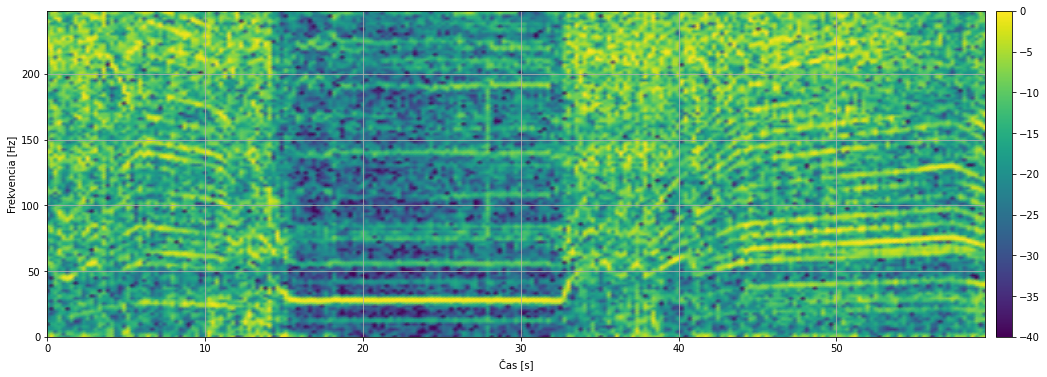
\includegraphics[width=\textwidth]{figures/verification/L83-dataset-spectrum.png}
	\caption{Spektrogram záznamu z vozidla \emph{L83\_4940\_Alexyho\_Svantnerova.csv}}
\end{figure}

\begin{figure}[h]
	\centering
    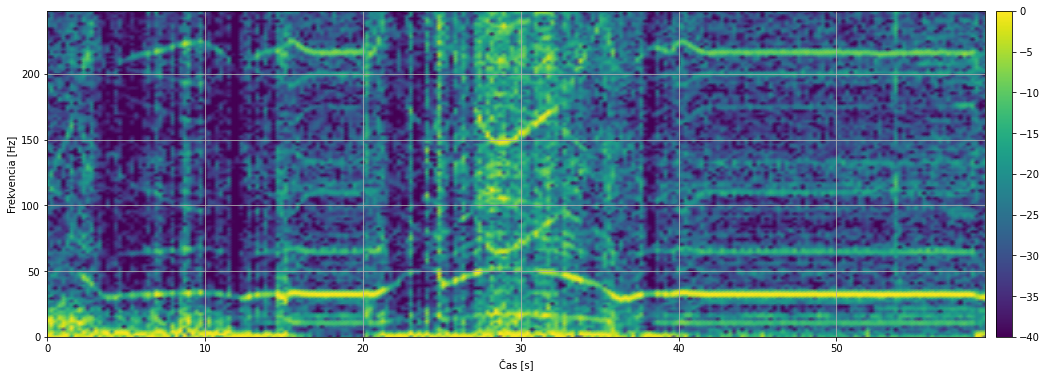
\includegraphics[width=\textwidth]{figures/verification/L35-dataset-spectrum.png}
    \caption{Spektrogram záznamu z vozidla \emph{L35\_1915\_Borska\_Zaluhy.csv}}
\end{figure}

Detekcia udalostí pri vzorkovacej frekvencii 500 Hz, dĺžkou FFT 256 bodov,
$t_{min} = 10$ a $t_{\Delta} = 4$ na datasete \emph{L35\_1915\_Borska\_Zaluhy.csv}:

\begin{figure}[h]
	\centering
    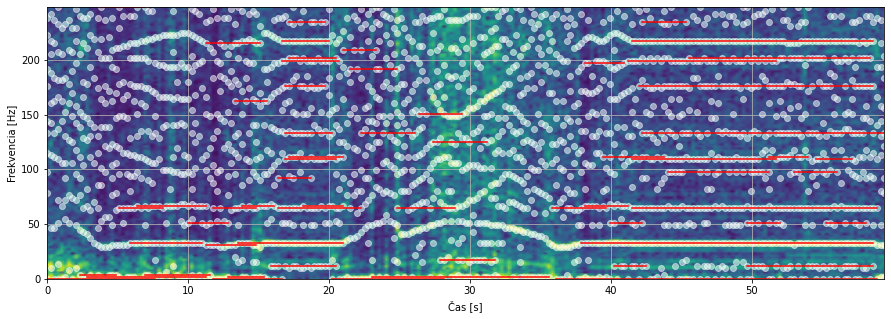
\includegraphics[width=\textwidth]{figures/verification/L35-dataset-A1.png}
    \caption{Algoritmus č.1: $k = 5$, $\epsilon = 0$, $h_{rel} = 8$}
\end{figure}

\begin{figure}[h]
	\centering
    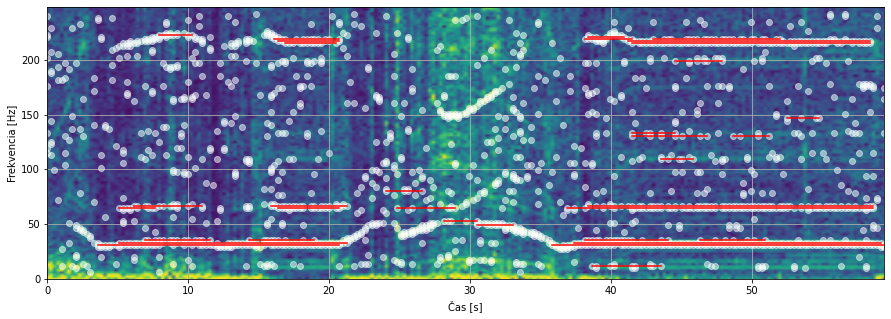
\includegraphics[width=\textwidth]{figures/verification/L35-dataset-A2.png}
    \caption{Algoritmus č.2: $k = 3$, $s = 7$}
\end{figure}

\begin{figure}[h]
	\centering
    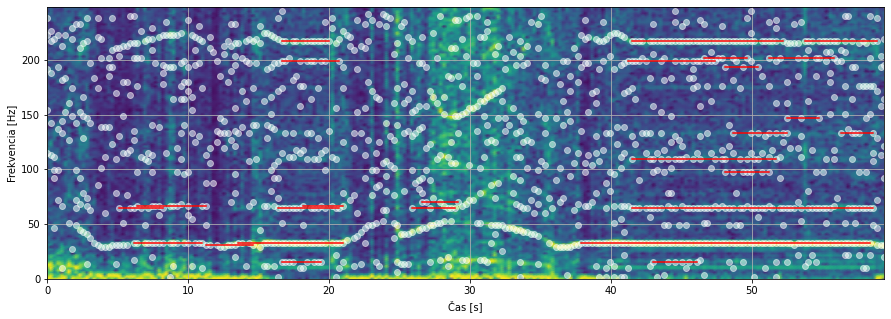
\includegraphics[width=\textwidth]{figures/verification/L35-dataset-A3.png}
    \caption{Algoritmus č.3: $t = 8$, $h = 1$, $p = 5$, $i = 0$}
\end{figure}


\thispagestyle{empty}
\setcounter{figure}{0}
\chapter{Obsah digitálneho média}
\pagenumbering{arabic}
\renewcommand*{\thepage}{E-\arabic{page}}
\par Evidenčné číslo práce v informačnom systéme: \RegNo
\par Obsah digitálnej časti práce (archív ZIP):
\par Názov odovzdaného archívu: BP\_MiroslavHajek.zip

\begin{itemize}[noitemsep]
\item[\textbf{>}] \textbf{firmware} - Zdrojový kód firmvéru senzorovej jednotky
	\begin{itemize}
	\item[\textbf{>}] \textbf{esp-dsp} - ESP DSP Library - knižnica na optimalizáciu spracovania signálov na ESP32.
	\item[\textbf{>}] \textbf{esp-idf} - Espressif IoT Development Framework - SDK pre hardvér ESP32.
	\item[\textbf{>}] \textbf{mpack} - MPack knižnica enkódera a dekódera MessagePack serializačného formátu.
	\item[\textbf{>}] \textbf{vibration-analyzer} - Samotná implementácia aplikačnej logiky.
		\begin{itemize}
		\item[\textbf{>}] \textbf{conf} - Konfiguračné súbory pre OpenLog (\emph{config.txt}), MQTT broker  (\emph{mosquitto.conf})
		a na zostavenie dokumentácie cez Doxygen (\emph{doxygen.conf}).
		\item[\textbf{>}] \textbf{docs} - Doxygen dokumentácia. Úvodná stránka je \emph{index.html}.
		\item[\textbf{>}] \textbf{main}
			\begin{itemize}
			\item[\textbf{>}] \textbf{include} - Hlavičkové súbory \emph{.h} aplikácie.
			\item[\textbf{>}] \textbf{src} - Zdrojové súbory \emph{.c} aplikácie.
			\end{itemize}
		\item[\textbf{>}] \textbf{tests} - Jednotkové testy na kontrolu najdôležitejšej funkcionality a validujúce konzistenciu
		medzi Python a C implementáciou algoritmov: \emph{test\_events.c} (test prúdového algoritmu nájdenia zmeny frekvencií),
		\emph{test\_peaks.c} (test klasifikátorov špičiek), \emph{test\_config.py} (test vzdialenej konfigurácie zariadenia).
		Nástroj na interaktívny vzdialený prístup k IoT jednotke \emph{config\_tool.py}.
		\end{itemize}
	\end{itemize}
\item[\textbf{>}] \textbf{measurements} - Analýza dátových sád a generovanie syntetických signálov v notebookoch \emph{.ipynb}.
	\begin{itemize}
	\item[\textbf{>}] \textbf{datasets} - Vibračné záznamy z vozidiel verejnej dopravy.
	\item[\textbf{>}] \textbf{experiments} - Pôvodné monitorovacie výpisy z experimentov slúžiace ako poklad na overenie riešenia.
		\begin{itemize}
			\item[\textbf{>}] \textbf{accuracies} - Úspešnosti klasifikácie na syntetickom spektrálnom profile. Súbor \emph{results.txt}.
			vychádza z analýzy v \emph{VibrationProcessingAlgorithms.ipynb}, do tabuľkovej podoby sa dostal v \emph{results-table.csv}.
			\item[\textbf{>}] \textbf{execution-algorithms} - Časy vykonávania jednotlivých algoritmov.
			\item[\textbf{>}] \textbf{execution-pipeline} - Časy vykonávania celej dátovej pipeline.
			\item[\textbf{>}] \textbf{memory-usage} - Spotreba flash pamäte.
			\item[\textbf{>}] \textbf{network} - Odchytená sieťová komunikácie z MQTT broker v \emph{.pcap} súboroch.
		\end{itemize}
	\item[\textbf{>}] \textbf{signals} - Užitočné funkcie ku prieskumnej analýze, vizualizácii a tvorbe modelov v Jupyter notebookoch.	
	\end{itemize}
\end{itemize}


\end{document}
